\documentclass[11pt,letterpaper,twoside,titlepage]{article}
\usepackage{array}
\usepackage[top=1in, bottom=1in, left=1in, right=1in]{geometry}
\usepackage{verbatim}
\usepackage{parskip}
\usepackage{graphicx}
\usepackage{amsmath}
\usepackage{attrib}
\usepackage{esint}
\usepackage{tipa}

\usepackage{tocloft}
\renewcommand{\cftsecfont}{}
\renewcommand{\cftsecpagefont}{}

% SECTION HEADINGS
\renewcommand{\thesection}{\arabic{section} }
\renewcommand{\thesubsection}{\arabic{section}.\arabic{subsection} }
\renewcommand{\thesubsubsection}{\arabic{section}.\arabic{subsection}.\arabic{subsubsection} }

\usepackage{titlesec}
\titleformat{\section}{\normalfont\bfseries\MakeUppercase}{\thesection}{0em}{}
\titleformat{\subsection}{\normalfont\bfseries}{\thesubsection}{0em}{}
\titleformat{\subsubsection}{\normalfont\bfseries}{\thesubsubsection}{0em}{}

\titlespacing{\section}{0pt}{0.5\baselineskip}{0pt}
\titlespacing{\subsection}{0pt}{0.5\baselineskip}{0pt}
\titlespacing{\subsubsection}{0pt}{0.5\baselineskip}{0pt}


% HEADER AND FOOTER
\usepackage{fancyhdr}
\pagestyle{fancy}
\fancyhf{}

\renewcommand{\sectionmark}[1]{\markright{\MakeUppercase{\thesection #1}}}
\renewcommand{\subsectionmark}[1]{}
\renewcommand{\subsubsectionmark}[1]{}

\fancyhead[LO,LE]{PHYS S211: General Physics I}
\fancyhead[RO,RE]{}
\fancyfoot[RO,LE]{\thepage}
\fancyfoot[LO,RE]{\rightmark}
\fancyfoot[CO,CE]{}

% MISCELLANEOUS CHANGES
\newcommand{\ds}{\displaystyle} % shortcut for displaystyle
\newcommand{\myrule}{\rule{\linewidth}{0.4pt}}

\author{Jason M. Amundson}
\title{PHYS S211: General Physics I}

\begin{document}
\maketitle

\pagenumbering{roman}
\tableofcontents
\addtocontents{toc}{~\hfill\textbf{Page}\par}
\clearpage
\pagenumbering{arabic}

% KINEMATICS
\section{Course overview}

\subsection{How do different disciplines view the world?}

\begin{figure}[h]
  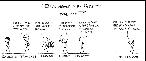
\includegraphics[width=\textwidth]{./figs/purity.pdf}
  \caption{From xkcd.com}
\end{figure}


\subsubsection{Biology}

(The focus here is on biology, but very similar comments could be made for geology and environmental science.)

Biology: The study of living organisms. The approach taken by biology is guided by and constrained by the fact that the subject is about living organisms.

Key constraints

\begin{enumerate}
\item Much of biology is {\bf complex}
  \begin{itemize}
    \item first steps are about identification, classification, and description of phenomena
    \item describe phenomena before looking for explanations of how it works
    \item huge vocabulary and many concepts to learn
  \end{itemize}

\item Biology depends on {\bf history}
  \begin{itemize}
  \item organisms are connected through a common, unbroken history that affects how things are today --- not the case for chemistry and physics
    \item evolution ``explains'' why a particular organism solves biological problem in a given way
  \end{itemize}
  
\item  Biology looks for {\bf mechanism}
  \begin{itemize}
    \item Not just ``What is life?'', but also and ``How does it work?''
    \item function of organs, genes, proteins and how do they affect organisms
  \end{itemize}
  
\item Biology is {\bf multi-scaled}
  \begin{itemize}
    \item organisms can be considered at many scales
    \item atomic and molecular scale (biochemistry)
    \item internal structure and functioning of organs (physiology)
    \item as part of large system in space (ecology) and time (evolution)
    \item relation between scales can be treated by reductionism or emergence --- going to smaller scales to explain something (reductionism), or seeing new phenomena arise as one goes to a larger scale (emergence)
  \end{itemize}
  
\item Biology is {\bf integrative}
  \begin{itemize}
   \item biological phenomena emerge from and must be consistent with the principles of chemistry, physics, and math
   \item chemistry and physics constrain how an organism can behave or evolve  
  \end{itemize}
\end{enumerate} 

\subsubsection{Chemistry}
Chemistry: The study of the composition and properties of substances and various elementary forms of matter.

Chemistry starts with the idea that all matter is made up of certain fundamental pieces (i.e., atoms) and is about the ways those elements combine to form more complex structures - molecules. But chemistry is not just about building molecules. It's about what you can do with that knowledge in our macroscopic world.

Key constraints:
\begin{enumerate}
\item Chemistry is about {\bf how atoms interact to form molecules} --- Understanding the basic principles of how atoms interact and combine is a fundamental starting point for chemistry.

\item Chemistry is about {\bf developing higher-level principles and heuristics} --- Because there are so many different kinds of molecules possible, chemistry develops higher-level ideas that help you think about how complex reactions take place.

\item Chemistry frequently {\bf crosses scales}, connecting the microscopic with the macroscopic, trying to learn about molecular reactions from macroscopic observations and figuring our what is possible macroscopically from the way atoms behave. The connections are indirect, can be subtle, and may involve emergence.

\item Chemistry often assumes a {\bf macroscopic} environment --- Much of what chemistry is about is not just idealized atoms interacting in a vacuum, but is about lots of atoms interacting in an environment, such as a liquid, gas, or crystal. In a water-based environment, the availability of H+ and OH- ions from the dissociation of water molecules in the environment plays an important role, while in a gas-based environment, the balance of partial pressures is critical.

\item Chemistry often {\bf simplifies} --- In chemistry, you often select the dominant reactions to consider, idealize situations and processes in order to allow an understanding of the most important features.

\end{enumerate}

For a chemist, most of what happens in biology (or geology or environmental science) is ``macroscopic'' --- there are lots and lots of atoms involved --- even though you might need a microscope to study it. In introductory chemistry you often assume that reactions are taking place at standard temperature and pressure (300 K and 1 atm).

\subsubsection{Physics}
Physics: The study of matter and its motion through space and time.

The goal of physics is to find the fundamental laws and principles that govern all matter --- including biological organisms. Those laws and principles can lead to many types of complex and apparently different phenomena.

Physics emphases four scientific skills that may seem different to what you see in introductory biology and chemistry classes but that are very useful:

\begin{enumerate}
\item Search for simplest possible example ({\bf ``toy model''})
  \begin{itemize}
    \item clearly illustrate key principles
    \item build-up from simple models to analyze more complex situations
  \end{itemize}
  
\item Physicists {\bf quantify} their view of the real world
  \begin{itemize}
    \item not satisfied until something can be quantified
    \item purely qualitative reason can be misleading
  \end{itemize}

\item Physicists {\bf think with equations}
  \begin{itemize}
    \item use equations to organize qualitative knowledge and to determine how things happen, what matters, and how much
    \item go back and forth between concepts and math
  \end{itemize}
  
\item Physicists deal with realistic situations by {\bf modeling and approximating}
  \begin{itemize}
    \item identify what matters most in a complex situation and create ``simple'' model
    \item the art of physics: figuring out what can be ignored without losing what you want to look at
    \item Einstein: ``Physics should be as simple as possible, but not simpler.''
  \end{itemize}

\end{enumerate}  

This way of doing science is a bit different from the way biology is often done --- but elements of this approach and the constraints imposed on biology by the laws of physics are becoming increasingly important.

\subsubsection{Math}
Math is a bit different from the sciences. What is math anyway??? How do mathematicians think about the world?

\begin{itemize}
  \item math is about relationships, patterns, logic
  \item abstract and rigorous
  \item not ``about'' anything in the physical world
  \item would math exist without humans?
  \item but --- a lot of relationships in science can be modeled by mathematical relationships
\end{itemize}

Math as taught in math classes often is primarily about the abstract relationships --- learning how to use the tools of math. Introductory physics is an excellent place to become comfortable with applying math to real world problems.


\subsection{Why physics?}
Why are you required to take physics?

Math majors: (1) apply your knowledge to ``real world'' problems and (2) gain an understanding of where the equations come from that you are learning how to solve and analyze

Biology / environmental science: (1) the core principles that control and organize our understanding of biology and the environment include physics and (2) the skills and competencies developed in physics are of great use in the life and environmental sciences, especially at the more advanced levels

Useful skills that we will focus on:
\begin{enumerate}
  \item {\bf Problem solving --- modeling and mechanistic reasoning:} 
    People are needed to figure out things that are not trivially obvious. Looking at a situation that is different from one you might have seen before, finding the similarities and differences, figuring out the knowledge and tools you need to resolve it, that's problem solving. A lot of what you will learn in this class will be through problem solving. Not just learning something and giving it back, but learning something and figuring out how to use it in new non-obvious situations.

    {\it I will not expect you to memorize equations for exams, and I may ask exam questions that differ somewhat from homework assignments.}

    \item {\bf Discourse --- learning to talk the talk:} 
      A critical idea in any science is that we use the community of scientists in a discipline to get a broader, more complete, and more accurate view of the world than any one individual can get. We're each limited in our experience and knowledge. Every scientific discipline relies heavily on the interaction of scientists with each other.

      {\it We will do a lot of in-class group work, both in lab and lecture. In addition, your homework will include problems that may be too hard and time-consuming for a single individual to do easily by themselves. You are encouraged to work in groups. The point of this is for you to learn to ``talk the talk'' --- to learn to ask questions of each other until you all understand what's going on better than any of you would individually.}
      
\item {\bf Stakes in the ground --- reasoning from principle:}
  Physics has been really good at finding universal (or near universal) principles that hold in a very wide variety of circumstances; things like energy conservation, conservation of charge, and Newton's laws --- our framework for describing and building models of motion.

  {\it By starting from basic principles and building upward, we will begin to make sense of complex knowledge in a coherent way.}

\item {\bf Quantification of experience --- mathematization, estimation, and scales:}
  All sciences are becoming increasingly quantitative. As a scientist you need to understand math and be able to interpret the implications of the math. Learning to use math in science (rather than just as pure math) can be quite tricky. Adding a physical interpretation to our symbols can actually change the way we think about the math.

{\it We'll use a lot of math of this course, so much that some of you may complain that physics is basically just another math course. (Some of you may also complain that we're not using enough calculus...) In some sense that's true. We will use math to solve scientific questions, and will also learn to estimate as a way to (1) determine ``what matters most'' and (2) check that our solutions make sense.}

\item {\bf Multiple-representation translation:} 
  All sciences represent the complex information that they convey in a variety of forms -- words, equations, pictures, graphs, and animations. The tricky thing is to learn to create a single enriched physical picture in your mind that blends all these different representations, linking them together.

{\it By focusing on ``simple'' situations, we'll gain an ability to think about science from multiple perspectives. We'll make sketches of physical processes, describe the processes using equations, and interpret the equations by drawing graphs.}

\item {\bf Understanding measurement:}
  All sciences rely heavily on measurement and data, none of which is perfectly reliable. Every experiment or measurement includes some model, both of the system being measured and of the process yielding the measurements. Understanding how measurement works --- and therefore what the measurement tells you, when it can be trusted, and when it can go astray --- is very important to a practicing scientist.

  {\it We'll gain a better understanding of measurements and data through lab experiments, which will illustrate that even simple systems can involve complex issues of measurement.}
  
\end{enumerate} 

You'll also work on developing these skills in your upper-division classes. Physics is a great place to practice since physics digs down to underlying simple principles and universal constraints. The physics we are learning here is, in the end, rather simple.

%In this class we will show you how simple physical principles can also constrain complex living systems and offer simple constraints and a framework for thinking about biology. You will be introduced to a new, complementary way of thinking that will contribute to your understanding of the living world.



\clearpage

\section{Introduction to kinematics}
Objectives:
\begin{enumerate}
  \item Course overview
  \item Key terminology
    \item Graphing motion
\end{enumerate}

\subsection{Overview}
We'll start the semester by learning about kinematics. Kinematics is the description of motion, and has the same origins as the word cinema. In a few weeks we'll discuss dynamics, or causes of motion. When we combine kinematics with dynamics, we are studying mechanics. In introductory physics, we'll cover classical mechanics --- one of the oldest branches of science

Classical mechanics: large, slow moving objects\\
Quantum mechanics: small objects\\
General relativity: fast moving objects\\

[Insert diagram of physics disciplines.]
\vspace{5cm}

\subsection{Types of motion}
motion: change in object's position with time

trajectory: path along which an object travels

For now, we'll only worry about rigid body motion (i.e., no deformation).

Four special cases of motion:

\begin{itemize}
\item straight line
\item projectile motion (influenced by gravity)
\item circular motion (e.g., planets, satellites)
\item rotational motion
\end{itemize}

\clearpage
[Insert diagrams.]
\vspace{6cm}

For motion that does not involve deformation or rotation, we can use a \textit{particle model}. Models are simplifications of reality that allow us to focus on important physics. In a particle model, we assume that all of the mass of an object is focused at a single point and that the all parts of the object move in the same direction with the same speed. Particle models are a good approximation of rigid body motion. In class I'll often use particles and boxes to represent much more complicated objects.

\subsection{Terms used to describe motion}
\begin{itemize}
\item position = location of an object

[Insert 1-D diagram; where is the object on this line?]
\vspace{3cm}


position can be positive \textit{or} negative -- this is important\\
units = [L]

\item displacement = change in position, [L] 
$$\Delta{x}=x_f-x_i$$
Can be positive \textit{or} negative (give example).

\item average velocity = average rate of change of position, [L]/[T]
$$v=\frac{\Delta{x}}{\Delta{t}}=\frac{x_f-x_i}{t_f-t_i}$$
Velocity can ALSO be positive \textit{or} negative. What does the sign tell you?

\item average speed = magnitude of average velocity, [L]/[T], always positive

\clearpage
Example: plot of position vs. time

[Insert diagram.]
\vspace{4cm}

Average velocity during the first interval:
$$v_1=\frac{x_1-x_0}{t_1-t_0}\Rightarrow\mbox{ slope of a straight line}$$
$$v_1>0$$

Average velocity during the second interval:
$$v_2=\frac{x_2-x_1}{t_2-t_1}<0$$

Often, we are more interested in the instantaneous velocity -- which means that calculus will already come in handy! Anybody know how?
$$\boxed{v=\lim_{\Delta{t}\rightarrow{0}}\frac{\Delta{x}}{\Delta{t}}=\frac{dx}{dt}}\Rightarrow\mbox{ evaluate at some point in time}$$

In practice, data is not continuous, velocity calculated from data is an average over some time interval.

From the fundamental theorem of calculus, we can see how displacement is related to velocity. (We won't do a lot of work with integrals, this is mostly for completeness.)
$$v=\frac{dx}{dt}\Rightarrow \boxed{\int_{t_0}^{t_1}v\,dt = \int_{t_0}^{t_1}\frac{dx}{dt}\,dt=x(t_1)-x(t_0)=\Delta{x}}$$


\item average acceleration = average rate of change of velocity, [L]/[T$^2$]
$$a_{avg}=\frac{v_2-v_1}{t_2-t_1}=\frac{\Delta{v}}{\Delta{t}}$$
As with velocity, often we are interested in the instantaneous acceleration
$$a=\lim_{\Delta{t}\rightarrow 0}\frac{\Delta{v}}{\Delta{t}}=\frac{dv}{dt}$$
Sometimes written as a second derivative
$$a=\frac{dv}{dt}=\frac{d\frac{dx}{dt}}{dt}=\frac{d^2x}{dt^2}$$
Not surprisingly, given what we just saw with displacement,
$$\Delta{v}=\int_{t_0}^{t_1}a\,dt$$
Can also be positive \textit{or} negative. What does the sign mean?

Simple rule for determining whether an object is accelerating or decelerating:\\
If $a\cdot v>0$ the object is accelerating, if $a\cdot v<0$ the object is decelerating  
\end{itemize}

\subsection{Example problems}

\begin{itemize}
\item The position of a particle, in cm, is given by $x(t)=9.75+1.50t^3$. (i) Sketch the position, velocity, and acceleration curves. (ii) What is the velocity at $t=2$s? What is the acceleration at $t=2$s? 

  \vspace{5cm}

\item A ball rolls along a smooth track shown in the figure. Each segment of the track is straight, and the ball passes smoothly from one segment to the next without changing speed or leaving the track. Draw three vertically stacked graphs showing position, velocity, and acceleration versus time. Each graph should have the same time axis, the proportions of the graph should be qualitatively correct. Assume that the ball has enough speed to reach the top.

  \begin{figure}[h]
    \begin{center}
      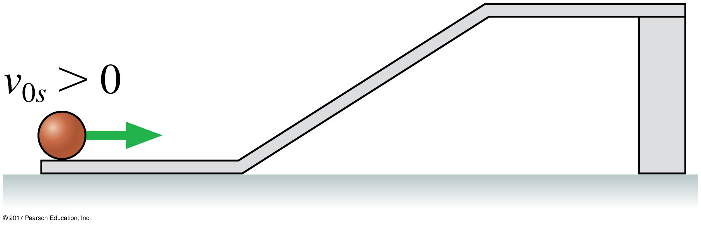
\includegraphics[]{./figs/P02_43_Figure.pdf}
    \end{center}  
  \end{figure}
  
  \end{itemize}

\clearpage

\section{Kinematic equations}
Objectives:
\begin{enumerate}
\item Transforming between displacement, velocity, and acceleration
\item Describing motion with graphs
\item Kinematic equations for constant acceleration  
\end{enumerate}

\hrulefill\\

Last class, I introduced the concepts of position, displacement, velocity, and acceleration.
\begin{itemize}
\item position: $x$ [L]
\item displacement: $\Delta{x}$ for large displacements, or $dx$ for infinitesimal displacements [L]
\item velocity: $v=\Delta{x}/\Delta{t}$ for average velocity, or $v=dx/dt$ for instantaneous velocity [L]/[T]
\item acceleration: $a=\Delta{v}/\Delta{t}$ for average acceleration, or $a=dv/dt=d^2x/dt^2$ for instantaneous acceleration [L]/[T$^2$]
\end{itemize}

In other words, we saw that velocity is the slope of the displacement curve, and acceleration is the slope of the velocity curve. 

[Insert diagram demonstrating that velocity is slope of displacement and acceleration is slope of velocity.]
\vspace{5cm}


I also briefly touched on the fact that you can calculate displacements if you know how the velocity varies with time, and similarly you can calculate changes in velocity if you know how the acceleration varies with time.

\textit{Transforming from velocity to displacement:}\\
$$\ds v=\frac{dx}{dt}\Rightarrow \int_{t_0}^{t_1}v\,dt=\int_{t_0}^{t_1}\frac{dx}{dt}\,dt=\Delta{x}=x_1-x_0$$
$$\ds x_1=\int_{t_0}^{t_1}v\,dt+x_0$$
If you don't know the initial position, $x_0$, you can't calculate the final position, $x_1$, just the change in position.\\

\textit{Transforming from acceleration to velocity:}\\
$$\ds a=\frac{dv}{dt}\Rightarrow \int_{t_0}^{t_1}a\,dt=\int_{t_0}^{t_1}\frac{dv}{dt}\,dt=\Delta{v}=v_1-v_0$$
$$\ds v_1= \int_{t_0}^{t_1}a\,dt+v_0$$
If you don't know the initial velocity, $v_0$, you can't calculate the final velocity, $v_1$, just the change in velocity.

Does anybody remember how you develop the idea of integral in calculus? Basically, by calculating the area under a curve. In other words, the change in velocity is the area under the acceleration curve and displacement is the area under the velocity curve.

[Insert diagram relating area under curves to change in velocity and displacement.]
\vspace{5cm}

\subsection{Kinematic equations for constant acceleration}
What I'd like to do for the rest of the class is to reinforce these relationships by analyzing the special case of constant acceleration. I'll do it two different ways: using calculus and by analyzing graphs. Constant acceleration is something that we see quite often in physics, so this isn't that unusual. Where would we see constant acceleration? A typical case is that we often assume that objects near the Earth's surface accelerate downward with a constant acceleration.

\subsubsection{Analysis using calculus}
This analysis is similar to what we did previously.
$$a=\frac{dv}{dt}\Rightarrow v=\int_{t_i}^t a\,dt^\prime = a(t-t_i) + v_0$$
Note that this is the equation for a straight line. Often we will simplify $t-t_i$ as $\Delta{t}$, which is the change in time, and we will similarly set $\Delta{v}=v-v_i$. This allows us to write
$$\boxed{\Delta{v}=a\Delta{t}+v_0}$$

Now let's calculate the displacement:
$$v=\frac{dx}{dt}\Rightarrow x=\int_{t_i}^t v\,dt^\prime$$
The velocity, $v$, is a function of time. So
$$x=\int_{t_i}^t a(t-t_i)+v_0\,dt^\prime=\frac{1}{2}a(t-t_i)^2+v_0(t-t_i)+x_0$$
Similar to what we did with the change in velocity, this will often be written as
$$\boxed{\Delta{x}=\frac{1}{2}a\Delta{t}^2+v_0\Delta{t}}$$

From these two equations we can create other useful equations. Solve the first equation for $\Delta{t}$,
$$\Delta{t}=\frac{v-v_0}{a}$$
and insert it into the second equation
$$\Delta{x}=\frac{1}{2}a\left(\frac{\Delta{v}}{a}\right)^2 + \frac{v_0\Delta{v}}{a}$$
Distribute and rearrange to arrive at
$$\boxed{2a\Delta{x}=v^2-v_0^2}$$
What is this equation missing? Time! Sometimes we don't know how long something takes but we know the initial and final states. The three equations that I just derived will be very useful for solving many problems that we encounter.

\subsubsection{Analysis using graphs}
Before applying the kinematic equations for constant acceleration, I want to show that the equations can also be derived by analyzing graphs.

For the case of constant acceleration,
$$a=\frac{\Delta{v}}{\Delta{t}}\rightarrow \Delta{v}=a\Delta{t} \rightarrow \boxed{v=a\cdot{t}+v_0}$$
Graphically, this looks like

[Insert constant acceleration graph.]
\vspace{5cm}

Note that the area under the curve is $a(t-t_i)$, which represents the change in velocity. Similarly, the area under the velocity curve is the displacement. We just saw the the velocity curve is a straight line. 

[Insert linear velocity graph.]
\vspace{5cm}

The area under the velocity curve consists of two parts: a rectangle and a triangle. Therefore,
$$\Delta{x}=v_0\cdot{t}+\frac{1}{2}\Delta{v}{t}$$
But we've already seen that $\Delta{v}=a\cdot{t}$, so this becomes
$$\Delta{x}=v_0t+\frac{1}{2}a\cdot t^2$$
which means that
$$\boxed{x=\frac{1}{2}a\cdot t^2+v_0t+x_0}$$

\subsection{Example problems}
Time to start working through problems. Let's start with somewhat conceptual problems.

[Insert graphs for graphical differentiation.]

[Insert graphs for graphical integration.]


\clearpage
%\hrulefill\\
Example problem (have students attempt it first):\\
A 747 has a length of 59.7 m. The plane lands on a runway that intersects another runway. The width of the intersection is 25.0 m. The plane decelerates through the intersection at 5.70 m/s$^2$ and clears the intersection with a final speed of 45.0 m/s. How long does it take the plane to clear the intersection.

Approach to solving problems:
\begin{enumerate}
\item Draw a diagram if applicable.
\item Write down what is known.
\item Write down what you want to find out.
\item Try to figure out what equations to use. This is often the most difficult part. Keep in mind what equations we have available to us. Often we will be making a choice from just a few equations. 
\item Solve problem algebraically as much as possible. This is easier than carrying numbers around, makes it easier for others (especially me) to figure out what you did, and sometimes results in a simple and elegant algebraic solution that gives you new insights into the problem.
\item After arriving at a solution, check that it makes sense.
\end{enumerate}

Given:\\
$x_i=0.0$ m\\
$x_f=25.0\mbox{ m }+\mbox{ }59.7\mbox{ m }=\mbox{ }84.7\mbox{ m}$\\
$v_f=45.0\mbox{ m/s}$\\
$a=-5.70\mbox{ m/s}^2$\\

Want to know $\Delta{t}$; note that $v_i$ is not given.

We can calculate $v_i$ from $2a\Delta{x}=v_f^2-v_i^2$.
$$v_i=\sqrt{v_f^2-2a\Delta{x}}$$
Then, using $a=\Delta{v}/\Delta{t}$,
$$\Delta{t}=\frac{\Delta{v}}{a}=\frac{v_f-v_i}{a}=\frac{v_f-\sqrt{v_f^2-2a\Delta{x}}}{a}=1.7\mbox{ s}$$

Does this make sense? How might you check? Use approximation and check units.



\clearpage

\section{Gravitational acceleration and projectile motion}
Objectives:
\begin{enumerate}
\item Motion due to gravitational acceleration
\item Vector descriptions of 2- and 3-dimensional motion
\item Kinematics of projectile motion
\end{enumerate}
\hrulefill

Last class I derived the kinematic equations for constant acceleration:
$$\Delta{v}=a\Delta{t}$$
$$\Delta{x}=v_i\Delta{t}+\frac{1}{2}a\Delta{t}\ds^2$$
$$v_f\ds^2-v_i\ds^2=2a\Delta{x}$$

\subsection{Gravitational acceleration: A special case of constant acceleration}
Free fall is an important example of motion under constant acceleration. Near the surface of the Earth, objects accelerate downward at about $g=9.81\mbox{ m/s}^2$ (ignoring the effects of air resistance).

\begin{enumerate}
\item $g>0$ (always positive); it is a \textit{magnitude}
\item If the coordinate system points upward, then $a=-g$; be careful to take into account the orientation of the coordinate system!
\item $g=9.81\mbox{ m/s}^2$ near the Earth's surface
\item Use kinematic equations for constant acceleration
\end{enumerate}

Demonstrations that gravitational acceleration is constant for all objects near the Earth's surface:
\begin{itemize}
\item Objects fall at roughly the same rate.
\item Tie washers to string and drop, demonstrating constant gravitational acceleration. Time interval from one washer hitting the ground to the next is constant; I calculated the spacing for the washers based on the assumption of constant acceleration. If washers are evenly spaced, the ``clicks'' increase in frequency.

Calculated spacing using based on:
$$v_i=0$$
$$a=-g=-9.81\mbox{ m/s}^2$$
$$\Delta{t} = 0.1\mbox{ s}, 0.2\mbox{ s},0.3 \mbox{ s},\dots$$
Replace $\Delta{x}$ with $\Delta{y}$. The spacing from the first washer to any of the subsequent washers is equal to $-\Delta{y}$, or in other words, the distance that the washers fall.
$$\Delta{y}=\frac{1}{2}g\Delta{t}^2=0.05\mbox{ m}, 0.20\mbox{ m}, 0.44\mbox{ m},\dots$$
\end{itemize}

Example:
A ball is shot vertically from the ground at a speed of 50 m/s. (1) What elevation will the ball reach? (2) How long will it take the ball to hit the ground? (3) What will its speed be when it hits the ground?

Given:\\
$v_i=50\mbox{ m/s}$\\
$x_i=0\mbox{ m}$\\
$a=-g=-9.81\mbox{ m/s}^2$

(1) The ball will have a speed of 0 m/s when it reaches its peak. Therefore,
$$v_{\mbox{peak}}\displaystyle^2-v_i^2=2a\Delta{y}$$
$$\Delta{y}=\frac{-v_i\displaystyle^2}{2a}=127\mbox{ m}$$

(2) To calculate the time to the peak, we'll again make use of the fact that $v_{\mbox{peak}}=0$.
$$a=\frac{\Delta{v}}{\Delta{t}}$$
$$\Delta{t}=\frac{\Delta{v}}{a}=\frac{v_{\mbox{peak}}-v_i}{a}=\frac{-v_i}{a}=5.1\mbox{ s}$$

(3)To calculate the speed when it hits the ground, we can use the kinematic equation that doesn't include $\Delta{t}$. That way we don't have to calculate how long it takes the ball to travel up and down.
$$v_f\displaystyle^2-v_i\displaystyle^2=2a\Delta{y}$$
Since $\Delta{y}=0$,
$$v_f\displaystyle^2=v_i\displaystyle^2$$
and so
$$v_f=\pm v_i.$$
The direction that the ball is travelling has changed, so 
$$v_f=-v_i=50\mbox{ m/s}.$$


\subsection{Motion in 2-dimensions}
We have mostly been using $x$ to define our coordinate system. The coordinate system can point in any convenient direction, and sometimes we will use $y$ or $z$ to indicate a distance along an axis.

We will often want to describe motion in 2-dimensions, and sometimes in 3-dimensions. In these instances we will need to use \textit{vectors}, and we will need to make use of $y$ and/or $z$. It is pretty straightforward to generalize what we have already learned to describe motion in 2- and 3-dimensions. Before continuing, we also need to remember what is meant by a vector.

Vector: a geometric quantity having both magnitude \textit{and} direction.

\clearpage
[Insert diagram of a vector.]
\vspace{5cm}

\begin{table}[h]
\begin{tabular}{lll}
\textbf{Kinematic variable} & \textbf{1D (scalar quantity)} & \textbf{2D (vector quantity)}\\
\hline
position & $x$ & $\vec{x}=\langle{x,y}\rangle$\\
displacement & $\Delta{x}$ or $dx$ & $\Delta\vec{x}=\langle{\Delta{x},\Delta{y}}\rangle$ or $d\vec{x}=\langle{dx,dy}\rangle$\\
velocity & $v=\frac{\Delta{x}}{\Delta{t}}$ or $v=\frac{dx}{dt}$ & $\vec{v}=\langle{v_x,v_y}\rangle=\langle{\frac{\Delta{x}}{\Delta{t}},\frac{\Delta{y}}{\Delta{t}}}\rangle$ or $\vec{v}=\langle{\frac{dx}{dt},\frac{dy}{dt}}\rangle$\\
acceleration & $a=\frac{\Delta{v}}{\Delta{t}}$ or $a=\frac{dv}{dt}$ & $\vec{a}=\langle{a_x,a_y}\rangle=\langle{\frac{\Delta{v_x}}{\Delta{t}},\frac{\Delta{v_y}}{\Delta{t}}}\rangle$ or $\vec{a}=\langle{\frac{dv_x}{dt},\frac{dv_y}{dt}}\rangle$\\
\hline
\end{tabular}
\end{table}

The kinematic equations for constant acceleration can also be written, and manipulated, in vector notation.
\begin{table}[h]
\begin{tabular}{ll}
\textbf{Motion in $x$-direction}\hspace{3cm} & \textbf{Motion in $y$-direction}\\
\hline
$\Delta{v_x}=a_x\Delta{t}$ & $\Delta{v_y}=a_y\Delta{t}$\\
$\Delta{x}=v_{x,i}\Delta{t}+\frac{1}{2}a_x\Delta{t}\ds^2$ & $\Delta{y}=v_{y,i}\Delta{t}+\frac{1}{2}a_y\Delta{t}\ds^2$\\
$v_{x,f}\ds^2-v_{x,i}\ds^2=2a_x\Delta{x}$ & $v_{y,f}\ds^2-v_{y,i}\ds^2=2a_y\Delta{y}$\\
\hline
\end{tabular}
\end{table}

We really haven't added all that much complexity here. All we're saying is that the equations that we developed for 1-dimensional motion can be generalized to describe motion in 2-dimensions. We can do this as long as the $x$- and $y$-axes are orthogonal/perpendicular to each other. For example, if an object moves in the $x$-direction, its $y$-position doesn't necessarily change at the same time. This doesn't mean that motion in the $x$-direction is independent of motion in the $y$-direction. 

[Insert diagram showing displacement vector. Should have $\vec{x_1}$ and $\vec{x_2}$]
\vspace{5cm}

Initial position: $\vec{x}_i=\langle{x_i,y_i}\rangle$\\
Magnitude: $\vec{x}_i=|\vec{x}_i|=\sqrt{x_i\ds^2+y_i\ds^2}$\\
Angle: $\tan\theta_i=y_i/x_i$\\
If angle is known: $x_i=\cos\theta_i$ and $y_i=\sin\theta_i$\\

After some time, the object moves to position $\vec{x}_f$. The displacement is $$\Delta\vec{x}=\vec{x}_f-\vec{x}_i=\langle{x_f,y_f}\rangle-\langle{x_i,y_i}\rangle=\langle{x_f-x_i,y_f-y_i}\rangle.$$ 
\textbf{You have to add or subtract vector components!} If this is confusing, ask questions and read your textbook. We will use vectors throughout the semester.

You can also add vectors graphically. Slide the tail of one vector to the tip of the other vector. For subtraction, the easiest way is to recall that subtraction is the same as adding a negative number. This applies also for vectors.

[Insert diagrams showing addition and subtraction of vectors.]
\vspace{5cm}

\hrulefill
\subsection{Projectile motion}
Projectile motion is a common example of motion in two dimensions, and is one in which we can treat the motion in the $x-$ and $y-$directions independently.

[Insert demo of falling marbles to show that vertical motion is independent of horizontal motion.]

\clearpage

\section{Projectile motion}
Objectives:
\begin{enumerate}
\item Solving projectile motion problems
\end{enumerate}

Last class we saw that the kinematic equations that we developed for motion in one direction can be easily generalized to describe motion in two or three dimensions. We'll work through a couple of projectile motion problems today.

\hrulefill
\subsection{Demos}
\begin{itemize}
\item Cart with shooting marble
\item Free-fall apparatus
\item Video of monkey getting hit by cannon
\end{itemize}

\subsection*{Cart with shooting marble}
Marble accelerates vertically but not horizontally. Demonstrates that for projectile motion problems we can often treat the x- and y-components of motion separately.

Assumptions:
\begin{itemize}
  \item Gravity is spatially constant and directed downward.
  \item Air resistance is considered negligible. (Air resistance depends on object's geometry and the medium through which it is travelling.)
\end{itemize}


\subsection*{Free-fall apparatus}

[Set-up free-fall apparatus.]

Which marble will hit the ground first? The one that falls straight down, or the one that is kicked by the spring?

Turns out that they hit the ground at the same time! They both start with no vertical velocity, and gravity acts downward on both marbles equally.

If we measure the height that the marbles are dropped from, and the distance that the projectile marble travels, can we calculate the marble's initial speed?

First, let's consider motion in the $y-$direction to determine the time it takes the marble to hit the ground.
$$\Delta{y}=v_{y,i}\Delta{t}+\frac{1}{2}a\Delta{t}\ds^2$$
But $v_{y,i}=0$, $\Delta{y}=-H$, and, if the $y$ points upward, $a=-g$.
$$-H=-\frac{1}{2}g\Delta{t}\ds^2$$
$$\Delta{t}\ds^2=\frac{2H}{g}$$
$$\Delta{t}=\sqrt{\frac{2H}{g}}$$

Now let's use the horizontal distance that the marble travelled to calculate its initial velocity. There is no acceleration in the $x-$direction.
$$v=\frac{\Delta{x}}{\Delta{t}}=\frac{\Delta{x}}{\sqrt{\frac{2H}{g}}}=\Delta{x}\sqrt{\frac{g}{2H}}$$

\subsection*{Video of monkey getting hit by a cannonball}
The cannon was pointed directly at the monkey. The speed with which the cannon was fired doesn't actually matter --- it only affects at what height the monkey gets hit. Can we prove that? What do we know? (By the way, this is kind of a tricky problem. I wouldn't ask a question like this on an exam unless I gave you a lot of hints.)

[Insert diagram of falling monkey.]
\vspace{5cm}

Let's start with the monkey:\\
$v_{y,i}=0$\\
$\Delta{y_m}=\frac{1}{2}a_y\Delta{t}\ds^2=-\frac{1}{2}g\Delta{t}\ds^2$\\
$\Delta{y_m}=H-y_m$, where $y_m$ is the monkey's position when it gets hit.

Now let's analyze the cannon:\\
$v_{x}=V_i\cos\theta=\frac{\Delta{x}}{\Delta{t}}$\\
$v_{y,i}=V_i\sin\theta$\\
$\Delta{y_c}=y_c-0=y_c=v_{y,i}\Delta{t}+\frac{1}{2}a_y\Delta{t}\ds^2=V_i\sin\theta\Delta{t}-\frac{1}{2}g\Delta{t}\ds^2$

We can make a few substitutions. Note that $\Delta{t}=\Delta{x}/(V_i\cos\theta)$. So, this means that
$$y_c=\frac{V_i\sin\theta}{V_i\cos\theta}\Delta{x}+(y_m-H),$$
which reduces to
$$y_c=\Delta{x}\tan\theta+y_m-H$$.
But $\tan\theta=H/\Delta{x}$... So,
$$y_c=\frac{H}{\Delta{x}}\Delta{x}+y_m-H=H+y_m-H=y_m.$$
When the cannonball has travelled a distance $\Delta{x}$, it will be at the same height above the ground as the monkey, and you will hear the monkey screach!


\subsection{Example problem}

You are throwing a ball from the top of a 10-m high cliff. You can throw the ball at a speed of $V_i=30\mbox{ m/s}$. At what angle relative to horizontal should you throw the ball to maximize the speed at which it hits the ground? Upward, downward, or horizontally?

For the $x-$direction, we have a constant velocity of
$$v_x=V_i\cos\theta$$

For the $y-$direction, we have
$$2a\Delta{y}=v_{y,f}\ds^2-v_{y,i}\ds^2$$
The velocity in the $y-$direction changes with time. $a=-g$, and $\Delta{y}=-10\mbox{ m}$.
$$2gH=v_{y,f}\ds^2-(V_i\sin\theta)\ds^2\Rightarrow v_{y,f}\ds^2=2gH+(V_i\sin\theta)\ds^2$$
We don't need to take the square root to find $v_{y,f}$, because we would want to square it in the next step.

The speed that the rock hits the ground at will be
$$V_f=\sqrt{v_x\ds^2+v_{y,f}\ds^2}$$
So, inserting the above results
$$V_f=\sqrt{V_i\ds^2\cos^2\theta+2gH+V_i\ds^2\sin^2\theta}=\sqrt{V_i\ds^2(\cos^2\theta+\sin^2\theta)+2gH} = \sqrt{V_i\ds^2+2gH}$$

It doesn't matter what angle you throw the ball at, just throw it fast!

This is a great example of why it pays off to do the algebra before plugging in any numbers. We ended up with an elegant, insightful, and surprising solution.


\clearpage

\section{Rotation of coordinate systems and relative motion}
Objectives:
\begin{itemize}
\item Rotation of coordinate systems
\item Motion as a vector
\item Relative motion
\end{itemize}
\hrulefill\\

The last couple of classes we've been talking about two-dimensional motion. We'll continue with that today by considering two more types of problems: motion along a ramp and relative motion.

To recap:
\begin{itemize}
\item Position, displacement, velocity, and acceleration are all \textit{vectors}. Rules for vector addition and subtraction apply. Vectors can, and often need to, be split into components that point in the $x$- or $y$-directions. Be sure that you understand the difference between $x$ and $\vec x$, $v$ and $\vec v$, $\ldots$
\item We have separate, but completely equivalent, sets of equations that describe motion in the $x$- and $y$-directions.
\end{itemize}

\subsection{Motion along a ramp}

One type of two-dimensional motion that we'll encounter frequently this semester is that of objects moving up or down ramps. So let's consider a box sliding down a ramp. For now we will ignore friction.

[Insert diagram of box sliding on a ramp.]
\vspace{5cm}

Gravity acts downward on the ramp, but the object will move along the ramp (not just vertically downward). To simplify the problem, we can make use of vector components and the fact that we are free to orient our coordinate system whatever way we choose. We will be turning a 2-dimensional problem into a one-dimensional problem.

Steps:\\
(1) Let $x$ point down the ramp, and $y$ point perpendicular up from the ramp.\\
(2) Split $g$ into vector components. One component points in the $+x-$direction, the other points in the $-y-$direction. Show that $a_x=g\sin\theta$.\\
(3) The ramp doesn't allow for motion in the $y-$direction, so we only have to deal with motion in the $x-$direction. This has become a one-dimensional problem.

\subsubsection{Example \#1}
Let's say that a box is released from a height of $H$, and that the ramp has an angle of $\theta$. What is the speed of the box when it reaches the end of the ramp? How long does it take to reach the end of the ramp?

Given:\\
$a_x=g\sin\theta$\\
$x_i=0$\\
$x_f=\frac{H}{\sin\theta}$\\
$v_i=0$\\

We want to know $v_f$. This is a problem where solving things algebraically can give great insights.

$$v_f\ds^2-v_i\ds^2=2a\Delta{x}=2g\sin\theta\frac{H}{\sin\theta}=2gH$$
$$\boxed{v_f=\sqrt{2gH}}$$

The final speed depends \textit{only} on the height from which the box is released!

$$\Delta{x}=v_i\Delta{t}+\frac{1}{2}a\Delta{t}^2=\frac{1}{2}a\Delta{t}^2$$
$$\Delta{t}=\pm\sqrt{\frac{2\Delta{x}}{a}}=\sqrt{\frac{2\frac{H}{\sin\theta}}{g\sin\theta}}$$
$$\boxed{\Delta{t}=\sqrt{\frac{2H}{g\sin^2\theta}}}$$

The time it takes to reach the end of the ramp does, however, depend on the angle of the ramp. 

\subsubsection{Example \#2}
A block slides along a frictionless track with speed $V=2\mbox{ m/s}$. Assume that it turns all corners smoothly with no loss of speed. What is the maximum height that the block reaches?
\clearpage
[Insert diagram of block on track.]
\vspace{5cm}

To solve this, we will rotate the coordinate system so that $x$ points up hill. This will become a one-dimensional problem.

Given:\\
$v_i=V$\\
$a=-g\sin\theta$\\
$\Delta{x}=\frac{H}{\sin\theta}$

If it just reaches the top of the hill, then $v_f=0$

We only need one equation to solve this.
$$2a\Delta{x}=v_f\ds^2-v_i\ds^2$$
$$-2g\sin\theta\frac{H}{\sin\theta}=-v_i\ds^2$$
$$2gH=v_i\ds^2$$
$$H=\frac{v_i\ds^2}{2g}=\frac{(2\mbox{ m/s})\ds^2}{2\times 9.81\mbox{ m/s}\ds^2}\approx 0.2\mbox{ m}$$

\subsubsection{Conceptual problem}
Imagine that a marble is rolling down a ramp that is sitting on a table. The marble leaves the end of the ramp, travels through the air, and hits the ground. Where will the marble hit the ground?

How would you solve this problem?
\begin{itemize}
\item Solve for speed of the marble when it reaches the end of the ramp.
\item Use result from (1) to calculate initial horizontal and vertical speeds for the projectile motion portion of the problem.
\item Solve for the time it takes the marble to hit the ground.
\item Calculate the distance that the marble travels through the air.
\end{itemize}

If we tried to do this problem right now, we'd overestimate the distance that the marble travels because we don't yet know how to account for \textit{rolling friction}. We'll come back to this problem later in the semester. 

\subsection{Relative motion}
In physics we often encounter problems where we need to know the motion of an object relative to another object. In order to talk about relative motion, we need to be comfortable with vectors. Should I review vectors again?

\begin{enumerate}
\item Motion of an object is always relative to some reference frame. 
\item Reference frames \textit{can} move. (If a reference frame is accelerating, then we have to use Einstein's theory or general relativity. Don't worry, we're not going to do that.)
\end{enumerate}

You've all experienced relative motion in one way or another. For example, if you're sitting in a parked car, and the car next to you starts to move, you sometimes get the sensation that you've started moving.

We are going to start with relative motion in one-dimension, because this is easier to understand than motion in two-dimensions.

Let's assume that Alex and Barbara each have their own reference frame; they are located at the origin of their reference frames. We will assume that Alex and Barbara are stationary.

[Insert diagram of Alex and Barbara and point P.]
\vspace{5cm}

For Alex, $P$ is at a positive position, whereas $P$ is at a negative position for Barbara. We can relate the relative position of $P$ to Alex with the relative position of $P$ to Barbara.
$$x_{pa}=x_{pb}+x_{ba}$$
The order of indices here matters --- $x_{pa}=-x_{ap}$. Why does this expression make sense?

Ok, so what if point $P$ is moving? Can we write down a similar expression using velocities? What are $v_{pa}$ and $v_{pb}$?
$$v_{pa}=\frac{\Delta{x_{pa}}}{\Delta{t}}$$
$$v_{pb}=\frac{\Delta{x_{pb}}}{\Delta{t}}$$
We already saw that $x_{pa}=x_{pb}+x_{ba}$, so
$$v_{pa}=\frac{\Delta(x_{pb}+x_{ba})}{\Delta{t}}=\frac{\Delta{x_{pb}}}{\Delta{t}}+\frac{\Delta{x_{ba}}}{\Delta{t}}=v_{pb}+v_{ba}=v_{pb}.$$
Alex and Barbara observe $P$ moving at the same speed (in this example).


\clearpage

\section{Relative motion and circular motion}
Objectives:
\begin{itemize}
\item Relative motion in 1D and 2D
  \begin{itemize}
  \item Emphasize that motion is always relative to a reference frame
  \item Opportunity to practice with 2D motion and vectors
  \end{itemize} 
\item Circular motion as a type of 1D motion
\end{itemize}
\hrulefill

\subsection{Galilean relativity}
reference frame = abstract coordinate system of an observer

Assumptions of Galilean relativity
\begin{itemize}
\item We will assume inertial reference frames (i.e., the observers are not accelerating relative to each other).
\item The reference frames share a universal time (i.e., time is not relative).
\end{itemize}
  
[Insert diagram illustrating relative position.]
\vspace{5cm}

Position:
$$\boxed{x_{BA}=x_{BP}+x_{PA}}$$

Take derivatives to find relative velocity:
$$\frac{dx_{BA}}{dt}=\frac{dx_{BP}}{dt}+\frac{dx_{PA}}{dt}$$
$$\boxed{v_{BA}=v_{BP}+v_{PA}}$$

If points $A$ and $B$ are moving with the same velocity, then $v_{BA}=0$ and
$$v_{PA}=-v_{BP}=v_{PB}$$
In other words, observers at $A$ and $B$ observe the object at $P$ moving with the same velocity.

We can take one more derivative to describe the relative acceleration.
$$\frac{dv_{BA}}{dt}=\frac{dv_{BP}}{dt}+\frac{dv_{PA}}{dt}$$
$$a_{BA}=a_{BP}+a_{PA}$$

In this class we will only concern ourselves with inertial reference frames. If we wanted to account for noninertial reference frames we'd have to incorporate Einstein's Theory of General Relativity. So for our purposes, $a_{BA}=0$, and thus
$$a_{PA}=-a_{BP}\Rightarrow \boxed{a_{PA}=a_{PB}}$$
In inertial reference frames, observers at $A$ and $B$ observe objects accelerating at the same rate.

We have derived these equations in one-dimension, but it is straight forward enough to discuss relative motion in two-dimensions.

$$\vec x_{BA}=\vec x_{BP}+\vec x_{PA}$$
$$\vec v_{BA}=\vec v_{BP}+\vec v_{PA}$$
$$0=\vec a_{BP}+\vec a_{PA}$$

\subsubsection{Example \#1}
A boat travels upriver at 14 km/h relative to the water. The water flows 9 km/h relative to the ground.

(a) What are the magnitude and direction of the boat's velocity relative to the ground?\\
(b) A child walks to from the bow to the stern at 6 km/h. What are the magnitude and direction of the child's velocity relative to the ground?

Have students work on these.

(a) Given: $v_{bw}=-14\mbox{ km/h}$; $v_{wg}=9\mbox{ km/h}$. Want to find $v_{bg}$.
$$v_{bg}=v_{bw}+v_{wg}=-14+9=-5\mbox{ km/h}$$
So the boat travels at $5$ km/h upstream.

(b) Given: $v_{bg}=-5\mbox{ km/h}$; $v_{cb}=6\mbox{ km/h}$. Want to find $v_{cg}$.
$$v_{cg}=v_{cb}+v_{bg}=6-5=1\mbox{ km/h}$$

\subsubsection{Example \#2}
You are trying to cross a river with a boat and would like to be exactly on the opposite side of the river. Your boat can travel 20 m/s (relative to the water). The river is flowing 2 m/s and is 1000 m wide. What angle should you leave shore at, and how long will it take you to reach the other side?

\clearpage
[Insert diagram showing what happens if you go straight across the river.]
\vspace{5cm}

If you head straight across the river, it will take you 50 s to cross the river ($\Delta{t}=\Delta{x}/v_x$), you will end up 100 m downstream from your objective.

[Insert diagram showing angle $\theta$.]
\vspace{5cm}

$$\vec{v}_{bw}+\vec{v}_{wo}=\vec{v}_{bo}$$
$$\langle{V\cos\theta,V\sin\theta}\rangle+\langle{0,-V_w}\rangle=\langle{V_o,0}\rangle$$

We want to find $\theta$ and $V_o$; the latter will tell us how long it takes to cross the river. This vector equation is the same thing as writing down two equations (with two unknowns).
$$V\cos\theta=V_o$$
$$V\sin\theta-V_w=0$$
From the second equation,
$$\theta=\sin\ds^{-1}\left(\frac{V_w}{V}\right)\approx 5.7^\circ$$
Inserting this into the first equation gives
$$V_o=19.9\mbox{ m/s}$$
So,
$$\Delta{t}=\frac{\Delta{x}}{V_o}=\frac{1000\mbox{ m}}{19.9 \mbox{ m/s}}=50.3\mbox{ s}$$

\subsubsection{Example \#3}
A hockey player is skating due south at 7.0 m/s. A puck is passed to him with a speed of 11.0 m/s and direction 22$^\circ$ west of south. What are the magnitude and direction (relative to due south) of the puck's velocity, relative to the hockey player?

Given:\\
$V_h=7.0\mbox{ m/s}$\\
$V_p=11.0\mbox{ m/s}$ at angle of $22^\circ$ west of south

We want to know $\vec{v}_{ph}$.

$$\vec{v}_{ph}=\vec{v}_{pi}+\vec{v}_{ih}=\vec{v}_{pi}-\vec{v}_{hi}$$
$$\vec{v}_{ph}=\langle{-V_p\sin\theta,-V_p\cos\theta}\rangle+\langle{0,-V_h}\rangle=\langle{-V_p\sin\theta,-V_p\cos\theta}\rangle-\langle{0,-V_h}\rangle$$
$$\vec{v}_{ph}=\langle{-V_p\sin\theta,-V_p\cos\theta+V_h}\rangle=\langle{-4.12,-17.2}\rangle$$

speed = 5.2 m/s\\
angle = 52.2$^\circ$ 




\clearpage

\section{Circular and rotational motion}
Objectives:
\begin{itemize}
\item Definitions and equations of circular and rotational motion
\item Relating circular motion and linear motion  
\item Example problems
\end{itemize}
\hrulefill

\subsection{Basic definitions and equations}
I introduced relative motion partially as a way of getting you comfortable with the fact that you can switch between reference frames or coordinate systems. One common case in which this occurs is very circular motion.

[Demo: ball on a string]

To describe motion around a circle, it is convenient to define position using the angle from the positive $x-$axis.

[Insert diagram defining $\theta$.]
\vspace{5cm}

Angular position is defined as $\theta=s/r$, in radians. Radians are \textit{not} units! However, it is sometimes convenient to report a measurement as being in radians so that it is clear that the number represents an angle. $\theta>0$ if counterclockwise from positive $x-$axis. Sometimes we will want to know the distance that an object has travelled along a circle, in which case we might use $s=r\theta$.

How do we convert between radians and degrees? $1\mbox{ rad}=\pi/180$

From here, we can probably guess how to define angular displacement, angular velocity, and angular acceleration.

Angular displacement: $\Delta{\theta}=\theta_f-\theta_i$\\
Angular velocity: $\omega=\frac{d\theta}{d{t}}$, [1/s]\\
Angular speed = $|\omega|$, [1/s]\\
Angular acceleration: $\alpha=\frac{d\omega}{d{t}}$, [1/s$^2$]

Like before, angular velocity is the slope of the angular position-versus-time graph, and angular acceleration is the slope of the angular velocity-versus-time graph. Conversely, angular displacement is the area under the angular velocity-versus-time graph, and the change in angular velocity is the area under the angular acceleration-versus-time graph. 

What is meant by positive or negative angular velocity? What is meant by positive or negative angular acceleration?

Sometimes we will need to convert between angular velocity (a.k.a. angular frequency) and frequency.
$$\omega=2\pi/T=2\pi f$$

I won't go through the derivations for the kinematic equations for circular motion because they are exactly analogous to what we did for one-dimensional motion. For constant angular acceleration:
$$\Delta\omega=\alpha\Delta{t}$$
$$\Delta\theta=\omega_i\Delta{t}+\frac{1}{2}\alpha\Delta{t}^2$$
$$\omega_f\ds^2-\omega_i\ds^2=2\alpha\Delta\theta$$
When $\alpha=0$, this reduces to
$$\Delta\theta=\omega\Delta{t}.$$

\subsection{Relating angular quantities to linear quantities}
Often we'll want to be able to convert between angular quantities and linear quantities. The derivation that I'm about to do should help to cement your understanding of vectors.

Note: The book arrives at these equations in a different, less elegant way.

For all of the following we will assume that the radius is constant.

\textbf{Position:}
$$x=r\cos\theta$$
$$y=r\sin\theta$$

Or, in vector notation:

$$\boxed{\vec x=\langle{r\cos\theta,r\sin\theta}\rangle}$$

\textbf{Velocity:}
$$\vec v=\frac{d\vec x}{dt}$$
$$\boxed{\vec v=\left\langle{-r\sin\theta\frac{d\theta}{dt},r\cos\theta\frac{d\theta}{dt}}\right\rangle=\langle{-r\omega\sin\theta,r\omega\cos\theta}\rangle}$$

The speed is the magnitude of the velocity:
$$v=|\vec{v}|=\sqrt{(-r\omega\sin\theta)^2+(r\omega\cos\theta)^2}=\sqrt{r^2\omega^2(\sin^2\theta+\cos^2\theta)}$$
$$\boxed{|\vec{v}|=|\omega| r} \mbox{ or, in shorter notation } \boxed{v=\omega r}$$


\textbf{Acceleration:}
$$\vec{a}=\frac{d\vec{v}}{dt}$$
$$\vec{a}=\left\langle{-r\cos\theta\left(\frac{d\theta}{dt}\right)^2-r\sin\theta\frac{d^2\theta}{dt^2}},-r\sin\theta\left(\frac{d\theta}{dt}\right)^2+r\cos\theta\frac{d^2\theta}{dt^2}\right\rangle$$

$$\boxed{\vec a=\left\langle{-r\omega^2\cos\theta-r\alpha\sin\theta,-r\omega^2\sin\theta+r\alpha\cos\theta}\right\rangle}$$

The acceleration consists of two parts: a component that cause the velocity vector to change direction (centripetal acceleration), and a component that cause the magnitude of the velocity vector to change (tangential acceleration).

Let's seperate the net acceleration into a centripetal acceleration and a tangential acceleration.

$$\vec a=\langle{-r\omega^2\cos\theta,-r\omega^2\sin\theta}\rangle+\langle{-r\alpha\sin\theta,r\alpha\cos\theta}\rangle=\vec{a}_c+\vec{a}_t$$

Note that the centripetal acceleration is non-zero as long as the object is moving in a circle. The tangential acceleration is only non-zero when the object's speed is changing.

[Insert diagram showing direction of the acceleration vectors, and pointing out that $\vec{a}_c$ always points inward and that $\vec{a}_c\perp\vec{a}_t$.]
\vspace{5cm}

The magnitude of the centripetal acceleration is
$$|\vec{a}_c|=\sqrt{(-r\omega^2\cos\theta)^2+(-r\omega^2\sin\theta)^2)}=\sqrt{r^2\omega^4(\cos^2\theta+\sin^2\theta)}$$
$$\boxed{a_c=\omega^2r=\frac{v^2}{r}}$$

The magnitude of the tangential acceleration is
$$|\vec{a}_t|=\sqrt{(-r\alpha\sin\theta)^2+(r\alpha\cos\theta)^2}=\sqrt{r^2\alpha^2(\sin^2\theta+\cos^2\theta)}$$
$$\boxed{a_t=\alpha r}$$

The centripetal acceleration and tangential acceleration are perpendicular to each other. This means that you can add them together to find the magnitude of the net acceleration by using the Pythagorean theorem.

$$a_{net}=\sqrt{a_c^2+a_t^2}$$
$$a_{net}=\sqrt{(\omega^2 r)^2+(\alpha r)^2}$$
$$\boxed{a_{net}=r\sqrt{\omega^4+\alpha^2}}$$

\subsection{Comments on rotational motion}
Everything that we've learned so far about circular motion also applies to rotational motion (i.e., the rigid body rotation of an object around some axis). An example of rotational motion is a bicycle wheel spinning around its axle. The fundamental difference between circular motion and rotation motion is that in rotational motion, all parts of an object DO NOT move at the same \textit{linear} speed/velocity. They do have the same angular velocity.

And all of the equations for circular motion can be easily adapted to rotational motion. So we know that the tangential speed is $v_t=\omega{r}$. The parts of the bicycle wheel that are farthest from axle move the fastest. 

If we want a fast bicycle, should we make the wheels big or small? (Actually its kind of a trick question, because big wheels are more difficult to turn!)

\subsection{Example problems}
\subsubsection{Example \#1}
Ex: The disk in a hard drive in desktop computer rotates at 7200 rpm. The disk has a radius of 13 cm. What is the angular speed of the disk?

Given:\\
$f=7200\mbox{ rpm}=120\mbox{ rev/s}$\\
$r=0.13\mbox{ m}$

$$\omega{r}=2\pi f=750\mbox{ s}^{-1}$$

\subsubsection{Example \#2}
The shaft of an elevator motor turns clockwise at 180 rpm for 10 s, is at rest for 15 s, then turns counterclockwise at 240 rpm for 12.5 s. What is the angular displacement of the shaft during this motion. Draw angular position and angular velocity graphs for the shaft's motion.

Angular velocity during the first interval: $\omega_1=-3\mbox{ rad/s}$\\
Angular displacement during the first interval: $\Delta\theta_1=\omega_1\Delta{t_1}=-30\mbox{ rad}$

Angular velocity during the third interval: $\omega_3=4\mbox{ rad/s}$\\
Angular displacement during the third interval: $\Delta\theta_3=\omega_3\Delta{t_3}=50\mbox{ rad}$

Net displacement: 20 rad

[Insert position-time and velocity-time graphs.]

\clearpage
\subsubsection{Example \#3}
You wrap a rope around the axle of a cart. The axle is 8 cm in diameter, and the wheels on the cart are 1 m in diameter. Assume that there is perfect friction between the rope and axle; in other words, the wheels roll when you pull on the rope without slipping. If you pull the rope at a constant 0.5 m/s, how quickly will the cart move (toward you!)? 

Given:\\
$r_{axle}=0.04\mbox{ m}$\\
$r_{wheel}=0.5\mbox{ m}$\\
$v_{t,axle}=1\mbox{ m/s}$

Want to know: $v$

How do we solve this? Let's first think about rolling motion.

[Insert diagram showing trajectory of a particle on the outside of the wheel.]
\vspace{5cm}

If the wheel rotates without slipping, during one revolution the center of the wheel will have moved forward a distance
$$\Delta x=v\Delta t=2\pi R,$$
and so
$$v=\frac{\Delta x}{\Delta t}=\frac{2\pi R}{\Delta t}.$$
Since the time to turn one revolution is the period, $T$, we find that
$$v=\frac{2\pi R}{T}.$$
Can we further simplify? Yes, we saw earlier that $\omega=2\pi/T$, so
$$\boxed{v=\omega R}$$
This is referred to as the rolling constraint.

An alternative way to derive this is using calculus.
$$v=\frac{dx}{dt}$$
In this case, the distance that wheel travels is the arclength of the wheel. Let $x=s$, so
$$v=\frac{ds}{dt}=\frac{d(r\theta)}{dt}=r\frac{d\theta}{dt}=r\omega$$

From this analysis we can also deduce that rolling motion is a combination of translation and rotation.

\clearpage
[Insert diagram of translation + rotation = rolling.]
\vspace{5cm}

Back to our example problem: once we calculate the angular velocity of the wheel, it is straightforward to calculate its speed.
$$v_{axle}=\omega r_{axle}$$
$$\omega=\frac{v_{t,axle}}{r_{axle}}=25\mbox{ rad/s}$$
$$v=\omega R=12.5\mbox{ m/s}$$
This is slightly faster than a person can run.

\clearpage


% DYNAMICS
\section{Newton's Laws}
Objectives:
\begin{itemize}
\item Types of forces
\item Newton's Laws
\item Free-body diagrams
\end{itemize}
\hrulefill

I spent the first seven lectures discussing \textit{kinematics}, which is the branch of physics that describes the motion of objects. We've talked about linear motion, two-dimensional motion, and circular/rotational motion. Today I'm going to start talking about \textit{dynamics}, which is the study of causes of motion and changes in motion. Kinematics and dynamics make up what we refer to as mechanics. We're now moving into the latter half of the 1600s, and we're adding a level of abstraction. We're also going to start being able to address much more interesting questions.

We are going to use the term \textit{force} to describe the agent that causes motion --- or as we'll see in a minute, changes in motion. We usually write force as $\vec{F}$. Force is a vector, just like displacement, velocity, and acceleration. Therefore it has a magnitude and direction, and can be split into vector components: $\vec{F}=\langle{F_x,F_y}\rangle$.

There are several different types of forces. We'll split them into two types: contact forces and body forces.

\begin{table}[h]
\begin{tabular}{ll}
Contact force & Body force\\
\hline
friction/drag & gravity\\
tension & electric\\
normal & magnetic\\
spring & \\
\hline
\end{tabular}
\end{table}

[Make sketches of the forces.]
\clearpage


\subsection{Newton's Laws}
In order to know how forces affect the motion of objects, we need Newton's Laws.

\subsubsection{Newton's First Law}
The velocity of an object remains constant unless it is acted upon by an \textit{external} force. In other words,
$$\sum\vec{F}=0\Rightarrow \vec{a}=0.$$
This is only valid for ``inertial'' references frames (i.e., non-accelerating reference frames). We will usually use reference frames that are not moving relative to the Earth. 

The first law is a formalization of Galileo's work on kinematics.

\subsubsection{Newton's Second Law}
The acceleration of an object is parallel and proportional to the net force acting on the object and inversely proportional to the object's mass.
$$\sum\vec{F}=m\vec{a}$$
From this, we see that force has units of [kg$\cdot$m/s$^2$], which we refer to as a newton [N]. This Law is based on the work of Galileo, Kepler, Brahe, and others.

This makes sense. Try pushing a penny and a piano. It takes much less effort to push a penny. Why? Because the penny has less mass. But what is mass???

Newton's First Law can be thought of as a special case of the second law: if $\vec{a}=0$, then $\sum \vec{F}=0$.

\subsubsection{Newton's Third Law}
For every action, there is an equal and opposite reaction. In other words, the force exerted on object 2 by object 1 is equal and opposite to the force exerted on object 1 by object 2.
$$\vec{F}_{12}=-\vec{F}_{21}$$

This is the most confusing of the three laws. A couple of examples:
\begin{itemize}
\item A hammer hitting a nail. The hammer exerts a force on the nail, and the nail exerts a force on the hammer. This is why hammers sometimes break.
\item A bug hitting a windshield. Which experiences a larger force --- the bug, or the windshield? They actually experience the same force, but the bug has a much smaller mass than the car, and so it undergoes an extreme acceleration!
\end{itemize}

\subsection{Demonstration of forces}
\begin{itemize}
\item Have student hold onto a spring while I pull on the other side. They should agree that they feel a pulling force.
\item Hang a mass from the spring. The spring stretches, so it must be exerting a force on the mass.
\item Hang a mass from the string. Is the string exerting a force on the mass? If I tied a rope around your waist and pulled, would you feel a force? Molecular bonds are essentially springs. The string does stretch a little bit, and that's what causes tension.
\item Place a book on the table. What forces are being exerted on the book? Is there actually a normal force acting upward on the book?
\item Place the book on top of a compression spring. The spring changes length, so it must be exerting a force on the book.
\item So we really can think of the normal force as being due to molecular bonds being compressed. Stand on table with laser beam pointing at the wall. Although they don't see the table deflect, they do see the position of the laser change. This is evidence that the table experienced compression.
\end{itemize}

\subsection{Free-body diagrams}
The key to solving problems using Newton's Laws is to draw free-body diagrams. The general method will be:
\begin{itemize}
\item Identify relevant forces in a free body diagram. A free body diagram is an illustration used to visualize the applied forces, movements, and resulting reactions on an object.
\item Use Newton's Second Law to set up 1 or 2 equations (motion in 1-D or 2-D). To do this, I always define forces as being positive, and then insert negative signs in Newton's Second Law if the force points in the negative $x$- or $y$-directions.
\item Solve for unknown terms. Sometimes this involves solving for acceleration and then applying kinematics to describe an object's motion.
\end{itemize}

Let's go through some examples. We'll draw free-body diagrams and identify the equations that we would use, but won't do anything more (yet).

A comment on systems: When drawing a free-body diagram and applying Newton's Laws, we are analyzing all of the \textit{external forces} acting on a \textit{system}. We are free to choose our system any way that we'd like.

\subsection{Example problems}
\subsubsection{Example \#1}
A box is resting on the floor.

Forces: Gravitational force pointing downward, and the normal force is pointing upward.

Equations:
$$\sum F_x=0$$
$$\sum F_y=F_n-F_g=ma_y=0$$
(For this particular problem, $F_n=F_g$.

\subsubsection{Example \#2}
A box is sliding down an inclined plane.

Forces: $\vec{F}_g$, $\vec{F}_k$, $\vec{F}_n$. Which way are they pointing?

Equations:
$$\sum F_x=F_g\sin\theta-F_k$$
$$\sum F_y=F_n-F_g\cos\theta$$

\subsubsection{Example \#3}
A box is pulled up a ramp by a falling mass that is connected by a string. For this problem, let's just identify the forces on the diagram.

Forces: $\vec{F}_g$, $\vec{F}_n$, $\vec{F}_k$, $\vec{F}_t$\\
To solve this type of problem, we need to balance forces on both objects. We'll discuss this in detail later. 

\subsubsection{Example \#4}
You are given two forces (draw vectors). Find the third force that would hold the object in equilibrium. The key to this problem is that for an object in equilibrium, $\sum \vec F=0$.


\clearpage

\section{Types of forces, part I}
Objectives:
\begin{itemize}
\item Gravitational forces
\item Normal forces
\item Tensional forces
\end{itemize}

\hrulefill

Last class I introduced Newton's Laws:
\begin{enumerate}
\item if $\sum\vec{F}=0\Rightarrow \vec{a}=0$
\item $\sum\vec{F}=m\vec{a}$
\item $\vec{F}_{ab}=-\vec{F}_{ba}$
\end{enumerate}
We then discussed how to use them to solve problems. The general approach is:
\begin{enumerate}
\item Draw a free-body diagram.
\item Insert forces into Newton's first or second law.
\item Do some algebra with one or more equations.
\item If necessary, use results to solve for an object's motion.
\end{enumerate}
We went through some conceptual examples, but didn't fully solve them because we didn't have a good understanding of the different types of forces. During the next couple of classes we will carefully go through some of the more common forces.

\subsection{Gravitational force}
Prior to Newton, it was known that
\begin{enumerate}
\item Objects near the Earth's surface fall with constant acceleration (Galileo)
\item Planetary orbits obey $T^2=cR^3$ (Kepler's third law)
\end{enumerate}
Newton supposed that all object's must obey the same physical laws, regardless of whether they were located on Earth or in space, and he reasoned that planetary orbits are a result of gravity. He was able to come up with an equation that could explain both of these phenomenon:
$$\boxed{F_g=\frac{Gm_1m_2}{r^2}},$$
where $F_g$ is the magnitude of the gravitational force, $G=6.67\times10^{-11}\mbox{ N}\cdot\mbox{m}^2\mbox{/kg}^2$, $m_1$ and $m_2$ are the masses of two objects, and $r$ is the distance between the objects' centers of mass. The gravitational force is directed along the line joining the two objects.

For objects near the Earth's surface, $m_1=m_{earth}=5.972\times 10^{24}\mbox{ kg}$ and $r\approx 6,371\mbox{ km}$. Therefore,
$$\frac{Gm_1}{r^2}\approx 9.81\mbox{ m/s}^2=g,$$
and so
$$F_g=mg,$$
where we've now defined $m$ as being the mass of an object near the Earth's surface.

Let's consider an object in free-fall. If we add up the forces acting on the object, we have
$$\sum F_y=-F_g=ma_y.$$
But since $F_g=mg$,
$$-mg=ma_y\Rightarrow \boxed{a_y=-g},$$
and so all objects fall with with constant acceleration (as long as we ignore the effects of air resistance). So Newton's Law of Gravitation explains Galileo's observations. It also explains Kepler's Law of Harmony. We can show this crudely by assuming that planets travel in circular orbits with constant speed. (We would need to use calculus to take into account the fact that planets have elliptical orbits.)

In order for a planet to travel in a circle, it must have some centripetal acceleration, $a_c$, that points toward the center of the orbit. From Newton's Second Law, we know that this acceleration must be caused by a force that points toward the center of the circle; we'll call that force a ``centripetal force''. If the centripetal force is due to gravity, then
$$F_g=ma_c.$$
We saw previously that $a_c=\omega^2 r$, and that angular frequency is related to orbital period through $\omega=2\pi/T$. Therefore, $a_c=(2\pi)^2r/T$ and as a result,
$$F_g=\frac{m(2\pi)^2r}{T^2}.$$
Substituting in for $F_g$,
$$\frac{Gm_1m}{r^2}=\frac{m(2\pi)^2r}{T^2}.$$
Cancelling like terms and re-arranging,
$$\boxed{T^2=\left(\frac{(2\pi)^2}{Gm_1}\right)r^3=kr^3}.$$

To reiterate, near the Earth's surface, use $F_g=mg$, and farther away use $F_g=\frac{Gm_1m_2}{r^2}$.

\subsection{Normal forces}
If a an object is sitting on the ground, there will be a gravitational force acting downward on the object and a normal force that keeps the object from moving through the ground. The normal force is always oriented normal (i.e., orthogonal) to the surface and it adjusts its magnitude to keep the object from moving through the surface.

\clearpage
[Insert free-body diagram of box sitting on the ground.]
\vspace{5cm}

You can think of this force like a stiff spring under compression. The molecules in the ground are being compressed, and so they respond by pushing upward. The normal force prevents the object from moving through ground. In this simple example, we have
$$\sum F_y=F_n-F_g=0$$
$$F_n=F_g=mg$$
(Note that it is not generally true that $F_n=mg$.)

\subsection{Tensional forces}
Tensional forces are similar to normal forces in the sense that they are a response to other forces. You can think of tension as being like a stiff spring under extension. The molecular bonds in the rope or string are stretched just a little bit, and they are trying to return to their equilibrium lengths.

[Insert diagram of mass hanging from a string.]
\vspace{5cm}

In the above diagram, there are two forces acting on the hanging mass: gravity and the tensional force from the string. According to Newton's second law, 
$$\sum F_y=F_t-F_g=ma_y=0,$$
so
$$F_t=F_g=mg.$$
The larger the mass, the greater the tensional force (i.e., the tensional force adjusts its magnitude --- until the string breaks!). We will often use the ``massless string approximation'', which allows us to set the tensional force constant throughout a string. To see why we can do this, let's consider 
the same problem as before, but now let's calculate the tensional force at the top of the string where it connects to the ceiling.

[Insert modified diagram of mass hanging from a string.]
\vspace{5cm}

Like before, we have
$$\sum F_y=F_t-F_g=ma_y=0,$$
and so
$$F_t=F_g=mg.$$
However, the mass $m$ now includes the mass of the object \textit{and} the mass of the string. In other words, $m=m_o+m_s$. Thus,
$$F_t=(m_o+m_s)g.$$
How important is $m_s$? If $m_o=100$ kg and $m_s=1$ kg, then the tension at the top of the rope will be 1\% larger than the tension at the bottom of the rope. For a lot of problems, that 1\% difference is irrelevant (especially considering errors associated with lab experiments) and so we can ignore the mass of the rope.

\subsection{Example problems}
\subsubsection{Example \#1}
A box is pulled along a frictionless surface with a rope. The rope makes an angle $\theta$ with horizontal. Derive expressions for the normal force and the horizontal acceleration.

[Insert diagram.]
\vspace{5cm}

$$\sum F_x=F_t\cos\theta=ma_x$$
$$\boxed{a_x=\frac{F_t}{m}\cos\theta}$$

$$\sum F_y=F_n+F_t\sin\theta-F_g=ma_y=0$$
$$\boxed{F_n=F_g-F_t\sin\theta}$$
The normal force doesn't always balance gravity. It simply prevents the box from passing through the ground. In this case, tension in the rope decreases the normal force. Furthermore, two objects can be in contact but have $F_n=0$. In this problem, if $F_g=F_t\sin\theta$, then $F_n=0$. A normal force cannot cause an acceleration by itself, and thus $F_n\leq{0}$. 

\subsubsection{Example \#2}
A automobile engine has a weight of 3150 N. The engine is being positioned above an engine compartment. To position the engine, a worker is using a rope. Find the tension in the supporting cable and in the positioning rope. The cable is 10$^\circ$ from vertical, and the rope is 80$^\circ$ from vertical.

[Insert diagram.]
\vspace{5cm}

To solve this, think about the forces that are acting on the ring that connects the cable, the rope, and the engine.

$$\sum F_x = -T_1\sin\theta_1+T_2\sin\theta_2=0$$
$$\sum F_y = T_1\cos\theta_1-T_2\cos\theta_2-F_g = 0$$
From the first equation,
$$T_1=T_2\frac{\sin\theta_2}{\sin\theta_1}$$
Inserting this into the second equation,
$$T_2\frac{\sin\theta_2}{\sin\theta_1}\cos\theta_1-T_2\cos\theta_2-F_g = 0$$
$$T_2\left(\frac{\sin\theta_2}{\sin\theta_1}\cos\theta_1-\cos\theta_2\right)=F_g$$
$$T_2=\frac{F_g}{\frac{\sin\theta_2}{\sin\theta_1}\cos\theta_1-\cos\theta_2}\Rightarrow \boxed{T_2=582\mbox{ N}}$$
Plugging this result back into the expression for $T_1$ gives
$$\boxed{T_1=3.30\times 10^5\mbox{ N}}$$




\clearpage

\section{Types of forces, part II}
Objectives:
\begin{itemize}
\item Frictional forces: static vs. kinematic
\end{itemize}

Last class:
\begin{itemize}
\item Gravitational force: $F_g=\frac{Gm_1m_2}{r^2}$, but use $F_g=mg$ near the Earth's surface.
\item Normal force: $F_n>0$, points perpendicular to surface.
\item Tensional force: $F_t$, points in direction of string. Massless string approximation allows us to assume that the tensional force is constant through the string.
\end{itemize}

\subsection{Frictional force}
The normal force is very important when dealing with friction, which is known through experiments.

Consider the case in which the block is resting on a ramp. This means that friction balances whatever forces would tend to cause acceleration (in this case, down the ramp). 

[Insert diagram of boxing resting on a ramp.]
\vspace{5cm}

In our example, this would mean that
$$\sum F_x=F_g\sin\theta-F_s=ma_x$$
where $F_s$ refers to static friction. Summing the forces in the $y-$direction,
$$\sum F_y=F_n-F_g\cos\theta=0\Rightarrow F_n=F_g\cos\theta \Rightarrow F_g=\frac{F_n}{\cos\theta}$$
Plugging this into the $x-$equation,
$$F_n\frac{\sin\theta}{\cos\theta}-F_s=F_n\tan\theta-F_s=ma_x$$

The frictional force (for static friction) will adjust its magnitude to hold the block in place until a certain threshold is reached will be in static equilibrium until a certain threshold is exceeded. For small angles, $F_s=F_n\tan\theta$ and therefore $a_x=0$. When the angle becomes too large, the box starts to slide. Thus, the maximum force of static friction is
$$\boxed{\max F_s=\mu_s F_n}$$
where $\mu_s=\tan\left(\theta_{max}\right)$ is the coefficient of static friction. It is a system property.

What if the box starts sliding?

[Insert diagram.]
\vspace{5cm}

We can solve for the frictional force.

Summing the forces in the $y$-direction:
$$\sum F_y = F_n-F_g\cos\theta=ma_y=0$$
$$F_n=F_g\cos\theta$$

Summing the forces in the $x$-direction:
$$\sum F_x=F_g\sin\theta-F_k=ma_x\neq 0$$
$$F_k=m(a_x-g\sin\theta)$$

This means that we can measure $F_n$ and $F_k$ experimentally. If we do lots of experiments, we find that $F_k$ is proportional to $F_n$.

[Insert diagram of $F_k$ vs. $F_n$; plots as straight line with $y-$intercept of 0.]
\vspace{5cm}

This means that
$$\boxed{ F_k = \mu_k F_n}$$
where $\mu_k$ is the coefficient of kinetic friction. It is a constant for a given system (combination of surfaces) and is determined experimentally. This is just a model for friction; its actually quite a bit more complicated and is still an active area of research. People that study earthquakes worry about friction a lot!

What makes something have a high coefficient of friction?

Coefficients of friction are generally less than 1, but don't have to be.

If you want to solve a problem in which a box isn't sliding initially, do the following:
\begin{enumerate}
\item Calculate the force that will tend to accelerate the box.
\item Does this force exceed $\max F_s$? If no, then immediately have the frictional force $F_s$. If yes, then the box will start sliding and you will have frictional force $F_k=\mu_k F_n$.
\end{enumerate}
In general, $\mu_s>\mu_k$. In other words, its easier to keep an object moving than it is to get it moving in the first place.

\subsection{Example problems}
\subsubsection{Example \#1}
You pull a box with a rope across a horizontal surface. The box is initially at rest, but you are able to overcome the maximum static friction. Plot the frictional force as a function of time. Let $m=100\mbox{ kg}$, $\mu_s=0.3$, and $\mu_k=0.2$.

[Insert diagram.]
\vspace{5cm}

Before and after the box starts moving,
$$\sum F_y = F_n-F_g=0\Rightarrow F_n=F_g=mg$$

Before the box starts moving,
$$\sum F_x=F_t-F_s=0\Rightarrow F_s=F_t$$

Let's assume that we linearly increase $F_t$ until the box starts moving. This occurs once $F_t\geq \max F_s=\mu_s F_n=\mu_s mg=0.3\times 100\mbox{ kg}\times 9.81\mbox{ m/s}^2\approx 300\mbox{ N}$. Once the box starts moving, we switch to kinetic friction: $F_k=\mu_k mg=0.2\times 100\mbox{ kg}\times 9.81\mbox{ m/s}^2\approx 200\mbox{ N}$.

\clearpage
[Insert plot of results.]
\vspace{5cm}

\subsubsection{Example \#2}
Demo to calculate the coefficient of friction of a block sliding over the table.

What do we need?

Forces on sliding block:
$$\sum F_x=F_t-F_k=m_1a_x$$
$$F_k=F_t-m_1a_x$$

$$\sum F_y=F_n-F_g=0\Rightarrow F_n=F_g$$

Forces on falling block:
$$\sum F_y=F_t-F_g=m_2a_y$$
$$F_t=m_2a_y+m_2g$$

$F_t$ on the falling block is the same as $F_t$ on the sliding block. We have an additional constraint, which is that $a_x=-a_y=a$.

So this means that
$$F_k=m_2a_y+m_2g-m_1a_x=m_2g-(m_1+m_2)a=\mu_kF_n=\mu_km_1g$$
$$\mu_k=\frac{m_2g-(m_1+m_2)a}{m_1g}$$

We need to measure the acceleration.
$$\Delta{x}=v_i\Delta{t}+\frac{1}{2}a\Delta{t}^2\Rightarrow a=\frac{2\Delta{x}}{\Delta{t}^2}$$

We can just as easily measure the vertical displacement.



\clearpage

\section{Types of forces, part III}
Objectives:
\begin{itemize}
\item Drag force
\item Terminal velocity
\item Spring force
\end{itemize}

\hrulefill

We have covered the following forces so far:
\begin{itemize}
\item Gravitational force: $F_g=\frac{Gm_1m_2}{r^2}$, but use $F_g=mg$ near the Earth's surface.
\item Normal force: $F_n>0$, points perpendicular to surface.
\item Tensional force: $F_t$, points in direction of string. Massless string approximation allows us to assume that the tensional force is constant through the string.
\item Frictional force: $F_k=\mu_kF_n$ for moving objects, where $\mu_k$ is the coefficient of kinetic friction, and $\max F_s=\mu_sF_n$ is the maximum force that can hold an object in equilibrium, where $\mu_s$ is the coefficient of static friction. If the force exerted on the object is less than $\max F_s$, the frictional force will exactly balance the sum of the other forces. Both $\mu_k$ and $\mu_s$ are dimensionless and determined experimentally.
\end{itemize}

Today I will introduce two more types of forces: drag, which I will just touch on briefly, and the spring force. Then the first half of next week we will discuss how forces affect circular and rotational motion: the centripetal force, apparent weight, and torque. %(Talk about pulleys in the context of torque? I think so.)

\subsection{Drag}
I just want to briefly touch on drag since it is something that we are all familiar with, and you are probably also familiar with the concept of terminal velocity. Now that we have a basic understanding of forces, we can discuss where the idea of terminal velocity comes from.

Drag is a really complicated subject because it deals with fluid dynamics and turbulence --- turbulence is still considered to be a pretty big mystery.

From experiments, though, we have a pretty simple expression that describes the drag force under certain circumstances:
\begin{enumerate}
\item The object is between a few millimeters and few meters in diameter.
\item The object's speed is less than a few hundred meters per second (100 m/s = 223 mph).
\item The object is moving through air near the Earth's surface.
\end{enumerate}
Under these circumstances, we can write that
$$\boxed{F_d=\frac{1}{2}C_D\rho Av^2}$$
where $F_d$ is the drag force, $C_D$ is a drag coefficient that depends on the object's shape, $\rho=1.22\mbox{ kg/m}^3$ is the density of air at sea level, $A$ is the cross-sectional area of the object, and $v$ is the object's speed. The drag force points opposite the direction of motion. For many objects, the drag coefficient is approximately 1/2. We'll assume that is the case, and so
$$\boxed{F_d=\frac{1}{4}\rho Av^2}.$$
The drag force increases with the square of the speed of the object!

Let's consider an object that is falling straight down.

[Insert diagram.]
\vspace{5cm}

There are two forces acting on the object, $F_g$ and $F_d$. They point in opposite directions. From Newton's second law,
$$\sum F_y=F_d-F_g=ma_y.$$
As the object accelerates, the drag force will become increasingly large and eventually $F_d$ and $F_g$ will cancel out (i.e., the object will stop accelerating, but it will not stop moving). When this happens
$$F_d-F_g=0\Rightarrow F_d=F_g.$$
Substituting in for $F_d$ and $F_g$ gives
$$\frac{1}{4}\rho Av^2=mg$$
$$\boxed{v_{\mbox{term}}=\sqrt{\frac{4mg}{\rho A}}}$$
What does this equation tell us?
\begin{enumerate}
\item If two different objects are the same size and shape, the heavier object will fall faster.
\item Cross-sectional area increases the drag and decreases the terminal velocity.
\item If we removed the Earth's atmosphere, the terminal velocity would go to $\infty$.
\end{enumerate}

Unfortunately, we can't really do anything more with drag without using calculus and differential equations. Let's see why by returning to the original force balance equation:
$$\sum F_y=F_d-F_g=ma_y$$
$$\frac{1}{4}\rho Av^2-mg=ma_y$$
We don't have the tools to solve this equation --- the acceleration is not constant --- so we can't compute the velocity as a function of time.

% include figure and discussion from Glimpses of Creatures in the Physical Worlds, if found...

\subsection{Springs}
When I started talking about types of forces, I used a spring to demonstrate the idea of a force and as an analogy for tensional forces and normal forces --- they can both be thought of as really stiff springs.

What do we know about springs? If you pull a spring, it will pull back in the opposite direction. If you push a spring, it will push back in the opposite direction. In other words, springs provide ``restoring forces''; they always try to return to the equilibrium length (i.e., the length they would be if there is no force being exerted on the spring). Furthermore, the magnitude of that force depends on how far the spring has been stretched or compressed. This was first shown by Robert Hooke, and curiously, published as a latin anagram: ``ceiiinosssttuv''. If you unscramble that, you come up with ``Ut tensio, sic vis'', meaning ``As the extension, so the force''. The way we write this nowadays is
$$\boxed{F_{sp}=-k\Delta{x}}$$
where $k$ is an empirical spring constant and $\Delta{x}$ is the displacement of the spring from equilibrium. The spring force points in the direction of the spring. This expression is referred to as Hooke's Law, though its not really a law because it breaks down if you stretch the spring too much. The notation can be a little bit confusing. Because the spring force can point either direction (depending on whether the spring is stretched or compressed), you need to use this formula to figure out the direction of the force.

[Insert several diagrams showing a spring being stretched or compressed, and discuss in terms of whether the force is positive or negative.]
\vspace{8cm}

Hooke's Law tells us that the force applied to a spring is linearly related to the displacement of the spring. So if we double the force, we double the displacement. As an example, let's consider a mass hanging from a spring.

\clearpage
[Insert diagram of mass hanging from a spring.]
\vspace{5cm}

If the system is in equilibrium, then the mass is not accelerating, and therefore
$$\sum F_y = F_s-F_g=0$$
$$-k\Delta{y}-mg=0\Rightarrow \Delta{y}=\frac{-mg}{k}<0$$
Why is $\Delta{y}<0$? Because the spring is being stretched in the negative $y$-direction.

[Insert diagram showing change in position of the end of the spring.]
\vspace{5cm}

Demo: If I double the mass, the displacement of the spring doubles (as long as my masses aren't too large!).

\subsection{Example problems}
\subsubsection{Example \#1}
A scale used to weigh fish consists of a spring hung from a ceiling. The spring's equilibrium (unstretched length) is 30 cm. When a 4.0 kg fish is suspended from the spring, it stretches to a length of 42 cm.

a) What is the spring constant?\\
b) What is the length of the spring if an 8.0 kg fish is hung from the scale?


$$\sum F_y=F_s-F_g=0$$
$$-k\Delta{y}-mg=0$$
$$k=\frac{mg}{-\Delta{y}}\Rightarrow \boxed{k=330\mbox{ N/m}}$$

Rearranging,
$$\Delta{y}=\frac{-mg}{k}=-0.24\mbox{ m}$$
The spring has been stretched downward by 24 cm. Its new length is therefore $\boxed{54\mbox{ cm}}$.

\subsubsection{Example \#2}
A toy train uses a spring to pull a 2.0 kg block across a horizontal surface. The train is motorized and moves forward at 5.0 cm/s. The spring constant has been measured to be 50 N/m, and the coefficient of static friction between the block and the surface is $\mu_s=0.60$. The spring is at its equilibrium length at $t=0$. Assume that at $t=0$, the train instantaneously accelerates from rest to 5.0 cm/s, and then moves forward at a constant rate. When does the block slip?

[Insert diagram.]
\vspace{5cm}

$$\sum F_y = F_n-F_g=ma_y=0 \Rightarrow F_n=F_g=mg$$
$$\sum F_x = F_{sp}-F_s=ma_x$$
Up until the time at which the block starts sliding, $a_x=0$. We want to find the time at which $F_{sp}=\max F_s$.
$$F_{sp}-\max F_s=0\Rightarrow F_{sp}=\max F_s$$
What is the spring force? The spring is being stretch by the train, so the force exerted by the spring on the train is $F_{sp}=-k\Delta{x}$. As the train moves to the right, the force pulling back on the train increases. (This means that the force exerted by the trains motor must also increase with time.) If the force exerted by the spring on the train is $-k\Delta{x}$, then the force exerted on the block is $k\Delta{x}$ (Newton's third law). Therefore,
$$k\Delta{x}=\max F_s=\mu_s F_n=\mu_s mg$$
$$\Delta{x}=\frac{\mu_s mg}{k}=0.235\mbox{ m}$$
How long does it take the train to go that distance?
$$\Delta{x}=v\Delta{t}\Rightarrow \Delta{t}=\frac{\Delta{x}}{v}=4.7\mbox{ s}$$


\clearpage

\section{Centripetal force}
Objectives:
\begin{itemize}
\item What causes circular motion?
\item True weight vs. apparent weight
\end{itemize}

\hrulefill

\subsection{Overview and demos}
We spent the last few lectures talking about different types of forces, and discussing how they affect linear motion. In the next two classes I'll talk about how forces cause circular and rotational motion by talking about the centripetal force (today) and torque (next class). The centripetal force is not really a new type of force --- rather, it is any force that causes an object to rotate in a circle. It can be a tensional force, as in the case of tetherball, or gravity in the case of a satellite orbiting the Earth.\\

Demo: Why doesn't the object move in a straight line? Identify the centripetal force. (1) Bucket full of water. (2) Object on the end of a string. (3) Object sitting on a rotating disk.\\


We've already seen that if an object is moving in a circle, the object's acceleration must point toward the center of the circle. We referred to this as the centripetal acceleration, and saw that
$$a_c=\frac{v^2}{r}=\omega^2r$$
A centripetal force, then, is any force that produces a centripetal acceleration. So
$$F_c=ma_c=m\frac{v^2}{r}=m\omega^2r$$
The one thing that makes centripetal forces difficult to deal with is that when we add up forces, we have to add them in up in the ``radial'' direction.

\subsection{Example problems}
\subsubsection{Example \#1}
One simple example of a centripetal force is a satellite orbiting the Earth.

[Insert diagram.]
\vspace{5cm}

If the satellite is far enough from the Earth we don't have to worry about drag (i.e., the satellite is not passing through the Earth's atmosphere). The only force acting on the satellite is gravity. Recall that
$$F_g=\frac{Gm_1m_2}{r^2}$$
In order for the satellite to stay in a circular orbit, this force must point toward the center of the circle (it does) and equal the centripetal force ($F_g=F_c$). So this gives
$$\frac{Gm_1m_2}{r^2}=m_2\frac{v^2}{r}$$
Rearranging, we find the orbital velocity:
$$\boxed{v=\sqrt{\frac{Gm_1}{r}}}$$

The International Space Station is 330 km above the Earth's surface, so $r=6371\mbox{ km}+330\mbox{ km} = 6671\mbox{ km}$. $m_1$ is the mass of the Earth, or $m_1=5.972\times 10^{24}\mbox{ kg}$, and $G=6.67\times 10^{-11}\mbox{ N}\cdot\mbox{m}^2/\mbox{kg}^2$. Therefore, its orbital velocity is 27,700 km/h.

Satellites are generally not entirely out of the Earth's atmosphere. Friction eventually slows them down, and so they crash to the Earth.

(Note that if we are close to the Earth's surface, and air resistance is ignored, then $v=\sqrt{gr}\approx 28500\mbox{ km/hr}$.)

\subsubsection{Example \#2}
As a roller-coaster car crosses the top of a 40-m-diameter loop-the-loop, its apparent weight is the same as its true weight. What is the car's speed at the top? How does the apparent weight at the bottom of the loop-the-loop (assuming that the speed remains constant) compare to its true weight?

True weight: $F_g=mg$\\
Apparent weight: $F_n$; this is the force that you feel pushing against you. If you were on a free-falling elevator, your apparent weight would be 0 because you wouldn't feel the elevator pushing upward. 

At the top of the loop-de-loop, $F_g$ and $F_n$ are both pointing toward the center of the circle. Adding them up,
$$\sum F_r=F_g+F_n=ma_c=m\frac{v^2}{r}$$
Since the apparent weight is the same as the true weight, $F_g=F_n$, and so
$$2F_g=m\frac{v^2}{r}$$
$$2mg=m\frac{v^2}{r}$$
Rearranging,
$$\boxed{v=\sqrt{2gr}=20\mbox{ m/s}}$$

At the bottom of the loop-de-loop,
$$\sum F_r=F_n-F_g=ma_c=v\frac{v^2}{r}$$
$$F_n=F_g+m\frac{v^2}{r}=mg+m\frac{v^2}{r}$$
$$\frac{v^2}{r}=2F_g$$
So, this means that
$$\boxed{F_n=F_g+2F_g=3F_g}$$

\subsubsection{Example \#3}
A 75 kg person weighs themselves at the north pole and at the equator. Which scale reading is higher, and by how much? Assume that the Earth is a perfect sphere.

At the north pole, the person just spins in a circle. There is no centripetal acceleration. Therefore, summing the forces gives
$$\sum F_r=F_g-F_n=ma_c=0$$
$$F_n=F_g=ma=735.8\mbox{ N}$$

At the equator, the person travels with in a circle, and so there is a centripetal force.
$$\sum F_r=F_g-F_n=m\omega^2r$$
$$F_n=F_g-m\omega^2r$$
The radius of the Earth is about $r=6.37\times 10^6\mbox{ m}$. It takes the Earth 86400 s to rotate once about its axis, and so $\omega=(2\pi)/(86400\mbox{ s})$. As a result, the apparent weight is about 2.5 N lower at the equator than at the pole.




\clearpage

\section{Torque}
Objectives:
\begin{itemize}
\item Definition of torque
\item Rotational equivalent of Newton's Second Law
\end{itemize}

\hrulefill

Last class we discussed how forces can produce uniform circular motion. Essentially, you need a force that produces a centripetal acceleration. This force can be any type of force or combination of forces that points toward the center of a circle.
$$\sum F_r=\frac{mv^2}{r}=m\omega^2r$$

Forces can also cause rigid bodies to rotate around some axis of rotation. We will use the term \textit{torque} to refer to the ability of a force to cause a rotation, and we'll define torque as 
$$\boxed{\tau=rF_\perp=rF\sin\theta}$$
where $\tau$ is torque and has units of N$\cdot$m, $r$ is the radial distance from the axis of rotation to the point at which the force is being applied, and $F$ is the force, and $\theta$ is the angle between the radial line and the line of action. Following standard conventions, $\tau>0$ for counter-clockwise rotation. The equation for torque can be thought of in two different, but equivalent ways.

\begin{itemize}
\item $\tau=r(F\sin\theta)$, where $F\sin\theta$ is the component of the force that acts perpendicular to the radial line.
\item $\tau=(r\sin\theta)F$, where $r\sin\theta$ is the lever arm, or perpendicular distance from the axis of rotation to the line of action.
\end{itemize}

[Insert diagram showing alternative view points.]
\vspace{5cm}


Although the concept of torque is a little bit strange, its something that we can easily test.

\clearpage
[Demo of object hanging on a rod.]
\vspace{3cm}



Consider the torque acting on a wrench: 

[Include diagram of the wrench and forces.]
\vspace{5cm}


If you apply force $F$ at a distance $r$ from the center of the bolt, and $r\perp F$, then you are exerting a torque $\tau=rF>0$.  If you exert the force at an angle $\theta=45^\circ$ relative to the radial axis, then $\tau=rF\sin\theta$ (in this case, $r\perp F\sin\theta$). If you double the radius, then $\tau=2rF$.

\subsection{Example problems: torque}
\subsubsection{Example \#1}
Two forces act on a rod that pivots about its center. Force $F_2$ is perpendicular to the rod and is a distance $l$ from the axis of rotation. Force $F_1$ has a magnitude of 20 N and is oriented at a 45$^\circ$ angle to the rod. The force is acting on the other side of the axis of rotation and at a distance of $2l$ from the axis. What should $F_2$ be so that $\tau_{net}=0$?

[Include diagram.]
\vspace{5cm}

$$\sum\tau=2lF_1\sin\theta-lF_1=0$$
$$F_2=2F_1\sin\theta=28\mbox{ N}$$

\subsubsection{Example \#2}
Various forces act on a rod. The rod can pivot around one of its ends. Rank the forces in order of smallest to largest torque.

[Insert diagram.]
\vspace{5cm}

\subsection{Rotational equivalent of Newton's second law}
Torque affects the rotational motion of an object. It is the rotational equivalent of force. To see how it affects motion, let's start with a really simple system consisting of a point mass, $m$, attached to a massless rod of length $l$. The rod can rotate around its end.

[Insert diagram.]
\vspace{5cm}

A force is exerted on the mass; the force is perpendicular to the rod. It therefore produces a tangential acceleration of the mass.
$$F_\perp=ma_t$$
Recalling that $a_t=\alpha r$,
$$F_\perp=m\alpha r.$$
Since $\tau=rF_\perp$,
$$\boxed{\tau = mr^2\alpha}$$

What about a system of particles, or a solid object?

\clearpage
[Insert diagram showing forces acting on a rotating object.]
\vspace{5cm}

The response of each particle is given by the torque acting on that particle. Thus, $\tau_1=m_1r_1\ds^2\alpha$, $\tau_2=m_2r_2\ds^2\alpha$, $...$ Because this is rigid body rotation, all points on the body have the same angular acceleration, $\alpha$. The net torque is $\tau_{net}=\tau_1+\tau_2+\tau_3+...$
$$\tau_{net}=\alpha\sum_{i=1}^Nm_ir_i\ds^2$$
The summation can only be calculated analytically for simple objects. So instead we replace the summation with
$$I=\sum_{i=1}^Nm_ir_i\ds^2,$$
where $I$ is the moment of inertia, giving
$$\tau_{net}=I\alpha$$
or equivalently,
$$\boxed{\sum\tau=I\alpha}$$
Does this look at all familiar? It is Newton's Second Law for rotation. The moment of inertia is a rotational equivalent to mass; it is an object's \textit{resistance to rotation}. Rotation about different axes of the same body yield different moments of inertia. The moment of inertia can be calculated for some objects, for others it must be measured. Some that can be calculated:

Solid cylinder: $I=\frac{1}{2}MR^2$\\
Thin-walled cylinder: $I=MR^2$\\
Solid sphere: $I=\frac{2}{5}MR^2$\\
Spherical shell: $I=\frac{2}{3}MR^2$

Note that they all have a dependence on mass and radius squared.

\subsection{Example problems: $\sum\tau=I\alpha$}
\subsubsection{Example \#1}
A 0.2 kg, 0.2-m-diameter disk is spun around its central axis by a motor. What torque must the motor supply to take the disk from 0 to 1800 rpm in 4.0 s?

$$\tau_{net}=\sum\tau=I\alpha$$
$$\alpha=\frac{\Delta\omega}{\Delta t}$$

Given:\\
$\omega_i=0$\\
$\omega_f=1800\mbox{ rpm}\times\frac{1\mbox{ min}}{60\mbox{ s}}\times\frac{2\pi}{1\mbox{ rev}}=188.5\mbox{ rad/s}$\\
$\Delta t=4.0\mbox{ s}$

So, from this $\boxed{\alpha=47.1\mbox{ rad/s}^2}$.

The moment of inertia can be calculated for a disk: $I=\frac{1}{2}mr^2=1\times 10^{-3}\mbox{ kg}\cdot\mbox{m}^2$.

Inserting into the expression for $\tau$, we get that $\boxed{\tau_{net}=0.05\mbox{ N}\cdot\mbox{m}}$.


\subsubsection{Example \#2}
How does a pulley affect the motion of a system? Consider an Atwood machine.
\clearpage
[Insert diagram.]
\vspace{5cm}

If we assume that the pulley is massless and frictionless, then we can assume that the tension is uniform in the rope. The force balance equations become

$$T-m_1g=m_1a$$
$$T-m_2g=-m_2a$$

We have two equations and two unknowns. Subtracting the second equation from the first equation gives
$$(m_2-m_1)g=(m_1+m_2)a\Rightarrow \boxed{a=\frac{(m_2-m_1)g}{m_1+m_2}}$$

If the pulley is not massless, but still frictionless, then we are no longer allowed to assume that the tension in the rope is uniform. Therefore,
$$T_1-m_1g=m_1a$$
$$T_2-m_2g=-m_2a$$
We have two equations and three unknowns. We need another equation, which comes from applying a torque balance to the pulley.

$$rT_1-rT_2=I\alpha=-I\frac{a}{r}$$

Dividing both sides by $r$,
$$T_1-T_2=-I\frac{a}{r^2}$$

Now subtracting the second equation from the first equation,
$$T_1-T_2+(m_2-m_1)g=(m_1+m_2)a$$
inserting the torque balance,
$$-I\frac{a}{r^2}+(m_2-m_1)g=(m_1+m_2)a$$
and rearranging,
$$\boxed{a=\frac{(m_2-m_1)g}{m_1+m_2+\frac{I}{r^2}}}$$

Is the last term in the denominator small compared to the other terms? If so, its okay to assume that the pulley is massless.


\subsection{Derivation of $\tau=rF_\perp$}
Define torque as the derivative of work with respect to the angular position $\theta$. (Force is similar defined as the derivative of work with respect to linear position.)
$$\displaystyle W = \int_a^b F\,ds$$
If the work is done along a circle, than $ds = rd\theta$ and therefore
$$\displaystyle W = \int_{\theta_a}^{\theta_b} rF_\perp\,d\theta$$
Because $\omega=d\theta/dt$, we can substitute in $d\theta=\omega dt$
$$\displaystyle W = \int_{t_a}^{t_b}rF_\perp\omega\,dt$$
The work has to equal the change in kinetic energy.
$$K = \sum\frac{1}{2}m_iv_i^2 = \sum\frac{1}{2}m_i\left(\omega r_i \right)^2 = \frac{1}{2}\omega^2\sum{m_ir_i^2} = \frac{1}{2}I\omega^2$$ 
and so
$$\frac{1}{2}I\left(\omega_b^2-\omega_a^2\right) =  \int_{t_a}^{t_b}rF_\perp\omega\,dt$$
Differentiating both sides with respect to time gives
$$I\omega\alpha = rF_\perp\omega$$
and therefore
$$\boxed{\tau\equiv rF_\perp = I\alpha}$$


\clearpage

\section{Torque, part II}
Objectives:
\begin{enumerate}
\item torque examples
\item rolling motion
\end{enumerate}

\hrulefill

\subsection{Review of torque}
Last class I introduced the idea of torque.
$$\tau=rF_\perp=rF\sin\theta$$

[Insert diagram showing definition of torque.]
\vspace{5cm}

All forces can generate torques, and the magnitude of the torque depends on (1) the distance from the axis of rotation to the point at which the force is acting and (2) the component of the force that is perpendicular to the radial axis. Torques are positive for counter-clockwise rotation.

We also saw that torques cause angular acceleration, such that
$$\sum \tau=I\alpha$$
where $I$ is the moment of inertia. $I$ can be thought of as an object's resistance to angular acceleration. This equation is Newton's Second Law for rotation.

Torque has many important consequences for physiology.
\begin{itemize}
\item If you stand with your toes against a wall, why can't you stand on your tip toes?
\item If you stand with your heels against a wall, why can't you pick up something off of the floor?
\item Two-legged animals ``fall over'' as they walk, but four-legged animals don't (think about center of mass)
\item Athletic position (low center of mass) makes you more stable; consider what happens if you are hit by a horizontal force?
\item Trees have to be able to support large forces and torques (due to the weight of the branches). This affects the development of trees --- apparently tree trunks are structurally different than branches.
  \item Muscles in your body exert torques on your limbs whenever you move.
\end{itemize}
    
Until now we've ignored objects' moments of inertia, e.g., when considering a motion of a pulley. Today I want to revisit Atwood's Machine, and then I'd like to go through a couple of more involved problems that involve the moment of inertia.

\subsection{Examples}
\subsubsection{Example \#1: Atwood's Machine}
Earlier in the semester I asserted that the tension in a string that passes over a pulley is uniform if we assume that the pulley is massless (and the axle is frictionless). Last class I said that the tension will be different on either side of the pulley if the pulley is not massless. It may not have been clear why that is the case, although in fact that is the general case.

[Insert diagram of pulley, indicating forces acting on it.]
\vspace{5cm}

Summing the torques acting on the pulley,
$$\sum \tau = rT_1-rT_2 = I\alpha$$
If the pulley is massless, then $I=0$ and therefore $T_1=T_2$, which is why we previously treated the tensions as being identical.

\subsubsection{Example \#2: A variation on Atwood's Machine}
In class we generally apply Newton's Laws in specific directions. We could also apply them in the direction of motion if we wanted to. For the case of Atwood's Machine, you could think of the hanging masses as a single system. The gravitational forces acting on the masses point either in the direction of motion or opposite the direction of motion.

When we solve the problem this way, we don't worry about the tensional forces in the string because they are \textit{internal forces} in the system. Internal forces are forces that are exchanged between objects in the system. We only need to worry about \textit{external forces}. What makes something an internal force or external force depends on how we define the system. When we solved this problem during the last class, we essentially treated the two masses and the pulley as separate systems, and so the tensional forces were external to each of those objects.

Instead of thinking about blocks hanging over a pulley, let's simplify the problem somewhat to think about a block being pushed over a roller that spins about an axle.

\clearpage
[Insert diagram of block on top of rolling object.]
\vspace{5cm}

The block has two forces acting on the ends, and in opposite directions. These are comparable to the gravitational forces in the Atwood Machine. There is also a force of static friction that keeps the block from sliding over the roller. We have previously implicitly assumed that the there is static friction between the pulley and the string.

Summing the forces in the $x-$direction gives
$$\sum F_x = F_1-F_2-F_s = ma$$
Here, the system only consisted of the block.

The force of static friction is also causing the roller to spin. Summing the torques on the roller,
$$\sum \tau = -rF_s = I\alpha$$
Here, the system only consisted of the roller.

The linear acceleration and angular acceleration must have the opposite sign (for this problem), and so $\alpha = -a/r$. Solving for $F_s$,
$$F_s = \frac{Ia}{r^2}$$

What happens if $a$ becomes really large? The block will start to slip over the roller, which is analogous to pulling a tablecloth really quickly. Now inserting $F_s$ into the first equation, we see that
$$F_1-F_2=a\left(m+\frac{I}{r^2}\right)$$
The moment of inertia of a cylinder/pulley is
$$I=\frac{1}{2}m_pr^2$$
and therefore
$$F_1-F_2=a\left(m+\frac{1}{2}m_p\right)$$
and the acceleration is
$$a=\frac{F_1-F_2}{m+\frac{1}{2}m_p}$$

The mass of the roller/pulley reduces the acceleration of the block.

What would have happened if we treated the system as including both the block and the pulley?

\subsubsection{Example \#3: Block pulled by falling mass}
A block is pulled by a string across a horizontal, frictionless plane. The other end of the string is suspended over a pulley and attached to a hanging mass. We will not assume that the pulley is massless but we will assume that the pulley is frictionless. Because the pulley has a moment of inertia, the tension in the two parts of the string are not necessarily equal. What is the acceleration of the block?

[Insert diagram.]
\vspace{5cm}

Start by summing the forces acting on mass $m_1$.
$$\sum F_x=T_1=m_1a_x$$
We want to find $a_x$. 
This is one equation with two unknowns. We need at least one more equation.

Now let's sum the forces acting on mass $m_2$.
$$\sum F_y=T_2-F_{g,2}=m_2a_y$$
Note that $a_x$ and $a_y$ have the same magnitude; $a_x>0$ and $a_y<0$, so $a_y=-a_x$. Therefore,
$$T_2-m_2g=-m_2a_x$$
We've introduced another equation, but also one more unknown. We now have two equations and three unknowns.

We can come up with a third equation by summing the torques on the pulley.
$$\sum \tau=rT_1-rT_2=I\alpha\Rightarrow T_2-T_1=I\frac{\alpha}{r}$$
This equation has given us yet one more unknown, $\alpha$. But we saw earlier that $a_t=\alpha r$, so $\alpha=a_t/r$. We need to be careful with the signs here. We have defined our torques to be positive for counter-clockwise rotation. We have also defined $a_x$ to be positive if it causes clockwise rotation. Therefore, we want to set $\alpha=-a_x/r$. Thus,
$$T_1-T_2=-I\frac{a_x}{r^2}$$
We have three equations and three unknowns. Let's solve the first two equations for $T_1$ and $T_2$, respectively, and insert them into the third equation.

$$T_1=m_1a_x$$
$$T_2=m_2g-m_2a_x$$

And so
$$m_1a_x-m_2g+m_2a_x=-I\frac{a_x}{r^2}$$
We want to solve this for $a_x$.
$$-m_2g=-m_2a_x-m_1a_x-I\frac{a_x}{r^2}=-\left(m_2+m_1+\frac{I}{r^2}\right)a_x$$
Finally, we arrive at
$${a_x=\frac{m_2g}{m_2+m_1+\frac{I}{r^2}}}$$

The moment of inertia of a disk is $I=(mr^2)/2$. If we treat the pulley as being a uniform disk of mass $m_p$, we can simplify the above equation to 
$$\boxed{a_x=\frac{m_2g}{m_2+m_1+\frac{m_p}{2}}}$$

Aside:

If you look back in your notes, you'll see that when we ignored the mass of the pulley, we arrived at
$$a_x=\frac{m_2g}{m_2+m_1}$$
Furthermore, if we plug this back into the original force balance equations, we see that 
$$T_1=\frac{m_1m_2g}{m_2+m_1}$$
and
$$T_2=m_2g-\frac{m_2^2g}{m_2+m_1}=\frac{m_2^2g+m_1m_2g}{m_2+m_1}-\frac{m_2^2g}{m_2+m_1}=\frac{m_1m_2g}{m_2+m_1}$$
In other words, if $m_p=0$ then $T_1=T_2$.

How much error do we introduce by assuming that $m_p=0$? Let's plug in some numbers to find out.

$m_1=0.2\mbox{ kg}$\\
$m_2=0.1\mbox{ kg}$\\
$m_p=0.01\mbox{ kg}$

$a_x\mbox{(with pulley's mass)}=3.22\mbox{ m/s}^2$\\
$a_x\mbox{(without pulley's mass)}=3.27\mbox{ m/s}^2$

That's an error of less than 2$\%$.

\subsubsection{Example \#4: Ball rolling down a ramp}
Let's consider a ball rolling down a ramp without slipping and try to predict where it will hit the ground once it flies through the air.

[Insert diagram.]
\vspace{5cm}

$$\sum F_x=F_g\sin\theta-F_f=ma $$

How do we deal with the frictional force? The ball isn't slipping, yet it is still moving...

$$\sum\tau=-rF_f=I\alpha $$
We have seen that $\alpha=a_t/r$. In this case, $a>0$ implies $\alpha<0$, so $\alpha=-a/r$ and therefore
$$-rF_f=-I\frac{a}{r}\Rightarrow F_f=I\frac{a}{r^2}$$
Inserting this into the above equation gives
$$F_g\sin\theta-I\frac{a}{r^2}=ma\Rightarrow a\left(\frac{I}{r^2}+m\right)=F_g\sin\theta=mg\sin\theta$$
$$a=\frac{mg\sin\theta}{\frac{I}{r^2}+m}$$
For a solid, uniform sphere, $I=(2/5)mr^2$. Thus,
$$a=\frac{mg\sin\theta}{\frac{(2/5)mr^2}{r^2}+m}=\frac{mg\sin\theta}{(2/5)m+m}=\frac{mg\sin\theta}{(7/5)m}$$
$$\boxed{a=\frac{5}{7}g\sin\theta}$$

If the ball starts at rest what will its speed be when it reaches the end of the ramp?

Recall:\\
$$v_r^2-v_i^2=2a\Delta{x}$$
$$v_r^2=2\frac{5}{7}g\sin\theta\frac{H}{\sin\theta}=\frac{10}{7}gH\Rightarrow \boxed{v_r=\sqrt{\frac{10}{7}gH}}$$

Previously, when we ignored rolling friction, we found that $v_r=\sqrt{2gH}$.

Now to solve the projectile motion problem:
$$v_{y,i}=-v_r\sin\theta$$
$$\Delta{y}=v_{y,i}\Delta{t}+\frac{1}{2}a_y\Delta{t}^2\Rightarrow 0 = \frac{1}{2}a_y\Delta{t}^2+v_{y,i}\Delta{t}-\Delta{y}$$
We can use the quadratic equation to solve for $\Delta{t}$
$$\Delta{t}=\frac{v_{y,i}\pm\sqrt{v_{y,i}^2+2a_y\Delta{y}}}{a_y}=\frac{-v_r\sin\theta\pm\sqrt{v_r^2\sin^2\theta-2g\Delta{y}}}{-g}$$

The horizontal distance that marble travels is 
$$\Delta{x}=v_{x,i}\Delta{t}=v_r\cos\theta\Delta{t}=v_r\cos\theta\frac{-v_r\sin\theta\pm\sqrt{v_r^2\sin^2\theta-2g\Delta{y}}}{-g}$$

Plug in numbers. How does this compare to our prediction if we had ignored rolling friction?

\textbf{Note:} This can also be solved by summing the torques around the axis of rotation (in the stationary reference frame) as opposed to using the reference frame that moves with the ball. This may be more intuitive to students, but it requires the use of the parallel-axis theorem.

[Insert sketch of box, octagon, and circle falling down a ramp.]
\vspace{5cm}

$$\sum\tau = -rF_g\sin\theta = I\alpha = \left(\frac{2}{5}mr^2+mr^2\right)\alpha$$
$$ -rmg\sin\theta = \frac{7}{5}mr^2\left(\frac{-a_x}{r}\right)$$
$$\boxed{a_x=\frac{5}{7}g\sin\theta}$$


\clearpage

\section{Static equilibrium}
Objectives:
\begin{itemize}
\item torque
\item static equilibrium
\item stability
\end{itemize}

\hrulefill

\subsection{Review of torque}
Spend the next couple of lectures discussing static equilibrium. First, I'll refresh your memory about torque and discuss gravitational torque by way of couple of demos.

First, review torque and discuss gravitational torque.

[Demo: meter stick rotates when it falls if one end is on the end of a table. This is due to gravity causing rotation around the axis of rotation.]

Torque on each element of the meter stick:
$$\tau=mgr=(\rho dr)gr=\rho g r\,dr$$
$$\tau_{net}=\ds\int_0^L\rho g r\,dr=\frac{1}{2}\rho gL^2=\frac{1}{2}mgL=mg\frac{L}{2}$$

The gravitational force can be thought of as being applied at the center of mass.

[Demo: pennies on a meter stick that falls. Why do some pennies detach from the meter stick as the stick rotates?]

$$\sum\tau=mg\frac{L}{2}=I\alpha$$
$$\alpha=\frac{a}{r}$$

So...
$$a=g\left(\frac{mLr}{2I}\right)$$

For a thin rod rotating about the axis,
$$I=\frac{1}{3}mL^2$$

$$\boxed{a=g\left(\frac{3}{2}\frac{r}{l}\right)}$$

\subsection{Static equilibrium}

I'd like to spend the next couple of lectures discussing equilibrium and elasticity --- two topics that we've briefly touched on. I won't really be introducing much new material.

What do we know about object's that are at rest?

$$\sum F_x = 0$$
$$\sum F_y = 0$$
$$\sum \tau = 0$$

These equations tell us that the an object is fixed in space relative to some reference frame that may or may not be moving.

We have already done problems where $\sum \vec{F}=0$. Now we'll also enforce that the objects don't rotate. We've already seen that $\tau=rF_\perp$. But if the object isn't rotating, what do we choose as our axis of rotation? Turns out that it doesn't matter, we pick any point that we want! We just have to be careful with the sign of the torques.

\subsection{Example problems}
\subsubsection{Example \#1: Person standing on a board}
A 64-kg person stands on a 2-m long board that is lying across two scales. Assume that the board is light (i.e., massless) and rigid. What are the readings on the scales when the person stands 0.5 m from one of the boards (and 1.5 m from the other)?

[Insert diagram.]
\vspace{5cm}

We need to add the forces and torques acting on the board.

The force-balance equations give us one equation and two unknowns:
$$\sum F_x = 0$$
$$\sum F_y = F_{n,1}+F_{n,2}-F_g=0$$

The torque balance gives us one additional equation. We are free to pick a convenient rotation axis. Let's pick a point where one of the unknown forces is acting.
$$\sum \tau = F_{n,1}\cdot{0}+F_{n,2}\cdot{2\mbox{ m}}-F_g\cdot{1.5\mbox{ m}}=0$$

We now have three equations and three unknowns ($F_g$ can be readily calculated). From the torque balance, we can find that
$$F_{n,2}=\frac{3}{4}F_g=\frac{3}{4}mg\Rightarrow \boxed{F_{n,2}=470\mbox{ N}}$$.

From the force balance,
$$F_{n,1}+\frac{3}{4}F_g-F_g=0\Rightarrow F_{n,1}=\frac{1}{4}F_g\Rightarrow \boxed{F_{n,1}=160 \mbox{N}}$$

\subsubsection{Example \#2: Ladder leaning against a wall}
A 3-m long ladder leans against a frictionless wall. The coefficient of static friction between the floor and the ladder is $\mu_s=0.2$. At what angle does the ladder start to slide?

[Insert diagram.]
\vspace{5cm}

Identify forces and sum the forces and torques.
$$\sum F_x = F_w-F_s=0 \Rightarrow F_s=F_w$$
$$\sum F_y = F_n - F_g=0 \Rightarrow F_n=F_g$$

We want to know at what angle does $F_w$ exceed $\max F_s$. Let's play with these equations for a minute before dealing with torque. We know that
$$\max F_s=\mu_sF_n=\mu_sF_g$$
So we need to know when $F_w$ exceeds $\mu_sF_g$.

When can calculate $F_w$ by summing the torques. We can pick any axis of rotation. What would be a convenient one here?
$$\sum \tau=-F_wl\cos\theta+\frac{1}{2}F_gl\sin\theta=0$$
$$F_w=\frac{1}{2}F_g\tan\theta$$

When is
$$\frac{1}{2}F_g\tan\theta > \mu_s F_g?$$
$$\tan\theta > 2\mu_s$$
$$\theta > \tan\ds^{-1}(2\mu_s)=21.8^\circ$$

We could also use this to calculate the coefficient of static friction (demo).


\subsubsection{Example \#3: Finding a meter stick's center of mass}
Demo: Use fingers to hold meter stick horizontally. Bring them together, and they will arrive at the stick's center of mass. Why?
\vspace{5cm}

\subsection{Stability}
Static equilibrium is very much related to the concept of stability. If you tilt an object, does torque due to gravity cause an the object to return to its original position or to tip over? The threshold is $\sum \tau =0$. When we think about torque due to gravity, keep in mind that gravity acts on an object's center of mass. What do I mean by center of mass?

[Insert diagrams of boxes tipping over.]
\vspace{5cm}

Consider the stability of a car.

[Insert diagram of a car with width $W$ and center-of-mass height $H$.]
\vspace{5cm}

When the car is just about to roll, the center of mass of the car is positioned directly above the wheels. In other words, the torque acting about that point is zero. The critical angle, $\theta_c$, at which this happens is related to $W$ and $H$:
$$\tan\theta_c=\frac{W/2}{H}\Rightarrow \theta_c=\tan\ds^{-1}\frac{W}{2H}$$

With a wider or shorter car, you have to tilt the car to a larger angle before it rolls over.

\clearpage

\section{Equilibrium and elasticity}
Objectives:
\begin{itemize}
\item Static equilibrium
\item Stability
\item Elastic deformation
\end{itemize}

\hrulefill

\subsection{Static equilibrium}
Last class we discussed problems involving static equilibrium. When an object is in static equilibrium,
$$\sum F_x=0$$
$$\sum F_y=0$$
$$\sum \tau=0$$
When calculating torques, you are free to pick any axis of rotation (the book refers to this as a ``pivot point'') that you'd like. Torque can be caused by any force, including gravity. Gravitational torque is especially important in the context of stability and balance. The gravitational torque is calculated by applying the gravitational force at the object's center of mass. OK, but what is meant by an object's center of mass?

Center of mass is the ``unique point where the weighted relative position of the distributed mass sums to zero''. There is a gravitational force acting downward on each point within an object. Adding up the torques produced by each of these forces is equivalent to applying the total gravitational force to the object's center of mass.

\subsection{Stability}
We can find the angle at which an object will tip over by calculating the torque as a function of the tilt angle. When $\tau=0$ the object is either completely stable or meta-stable. If it is meta-stable, tilting it a little bit one way or the other will cause it to topple.

[Insert diagram of a box about to tip over.]
\vspace{5cm}

\subsubsection{Example: Stability of a table}
How close can a 70-kg person stand to the end of a 56-kg table before it tips over?

[Insert diagram of the table. The edge of the table extends beyond the legs of the table.]
\vspace{5cm}

$$\sum F_x = 0$$
$$\sum F_y = F_{n,1}+F_{n,2}-F_{g,t}-F_{g,p}=0$$
$$\sum \tau = F_{g,t}l_1-F_{n,1}l_2-F_{g,p}L=0$$
Rearranging the torque balance gives
$$F_{n,1}=\frac{F_{g,t}l_1-F_{g,p}L}{l_2}=0$$
(When $F_{n,1}=0$, the table is just starting to tip.) Solving for $L$
$$L=\frac{F_{g,t}}{2F_{g,p}}=\frac{m_t}{2m_p}=0.4\mbox{ m}$$
$L$ is the distance from the leg of the table. The person can therefore stand 0.15 m from the end of the table.

\subsection{Elasticity}
So far in our analysis of static equilibrium we've assumed that objects maintain their shape. In reality, all objects stretch, compress, and deform. We've already talked about this a little bit in the context of normal forces and tensional forces, which are a result of compression and tension occurring at the molecular scale. These forces are ``restoring forces'' that try to restore the objects to their equilibrium position. Materials that have restoring forces are called ``elastic''. 

We can model these elastic restoring forces by treating them as springs.

What do we know about springs? If you pull a spring, it will pull back in the opposite direction. If you push a spring, it will push back in the opposite direction. In other words, springs provide ``restoring forces''; they always try to return to the equilibrium length (i.e., the length they would be if there is no force being exerted on the spring). Furthermore, the magnitude of that force depends on how far the spring has been stretched or compressed. As we've already seen, we write the restoring force of a spring as
$$\boxed{F_{sp}=-k\Delta{x}}$$
where $k$ is an empirical spring constant and $\Delta{x}$ is the displacement of the spring from equilibrium. The spring force points in the direction of the spring. This expression is referred to as Hooke's Law, though its not really a law because it breaks down if you stretch the spring too much. The notation can be a little bit confusing. Because the spring force can point either direction (depending on whether the spring is stretched or compressed), you need to use this formula to figure out the direction of the force.

[Insert several diagrams showing a spring being stretched or compressed, and discuss in terms of whether the force is positive or negative.]
\vspace{5cm}

Hooke's Law tells us that the force applied to a spring is linearly related to the displacement of the spring. So if we double the force, we double the displacement. 

When modeling elastic materials, we will replace $k$ with
$$k=\frac{YA}{L}$$
where $Y$ is Young's modulus (a material property), $A$ is the cross-sectional area of the object, and $L$ is the length of the object. An object with a large Young's modulus is resistant to changes in length.

When writing the elastic force, we often replace $\Delta{x}$ with $\Delta{L}$. So
$$F=-\frac{YA}{L}\Delta{L}=\Rightarrow \frac{F}{A}=-Y\frac{\Delta{L}}{L}$$
$F/A$ is the stress and $\Delta{L}/L$ is the strain (i.e., fractional change in length).

What does this equation tell us? What if we apply a large force to a thin rope? What if we construct a thicker rope out of the same material?

This equation also tells us that we should think about normal forces (and tensional forces) as being applied everywhere that two surfaces are in contact. However, instead of adding up a whole bunch of little forces, it is much easier to calculate the total force and apply it at the center of where two object's come in contact.

We were to make a plot of $F/A$ vs. $\Delta{L}/L$, we would find a linear relationship for small $\Delta{L}$. This is the range for which Hooke's Law is valid. Beyond that the material will remain elastic for a little bit more deformation until it reaches the elastic limit. Beyond that the material behaves plastically --- it changes length will very little change in force --- until it reaches the breaking point, or tensile/compressive strength.

[Insert diagram.]
\vspace{5cm}

Interestingly, some materials stretch a lot before breaking while others can only stretch a little bit. For example, steel and spider silk have similar tensile strengths (break at the same stress), but silk undergoes much more extension than steel.

[Insert diagram.]
\vspace{5cm}

Like torque, elasticity is also a very important concept in biology --- for example, it comes up in the context of extension and compression of bones.

\subsubsection{Example: Static equilibrium, torque, and elasticity}
Let's finish with an example problem that incorporates static equilibrium, torque, and elasticity.

A 100-kg, 3.5-m-long plank is supported on its end by a 7.0-mm-diameter rope with a tensile strength of 6.0$\times$10$^7$ N/m$^2$. How far along the plank, measured from the pivot, can an 800-kg piece of machinery be moved along the plank before the rope snaps?

[Insert diagram.]
\clearpage

We want to find at what point does $F_t/A=6.0\times 10^7\mbox{ N/m}^2$. The cross-sectional area is $A=\pi r^2=3.85\times 10^{-5}\mbox{ m}^2$, so we need to determine when $F_t=2310\mbox{ N}$.

$$\sum F_y=F_n-F_{g,p}-F_{g,m}+F_t=0$$
$F_t$ and $F_n$ are unknown, so we need one another equation. We want to remove $F_n$ from the first equation. The way to do this is to sum the torques around the point where the rope is holding up the plank. Let's call the length of the plank $L$, and the distance from the pivot to the machinery $l$.
$$\sum \tau=F_{g,p}\frac{L}{2}+F_{g,m}(L-l)-F_nL=0$$
$$F_nL=F_{g,p}\frac{L}{2}+F_{g,m}(L-l)$$
$$F_n=\frac{1}{2}F_{g,p}+F_{g,m}\left(1-\frac{l}{L}\right)$$
Let's plug the result into the force balance equation.
$$\frac{1}{2}F_{g,p}+F_{g,m}\left(1-\frac{l}{L}\right)-F_{g,p}-F_{g,m}+F_t=0$$
$$-\frac{1}{2}F_{g,p}-F_{g,m}\frac{l}{L}+F_t=0$$
Solve this for $l$; we want to find for what $l$ does $F_t=2310\mbox{ N}$.
$$F_{g,m}\frac{l}{L}=F_t-\frac{1}{2}F_{g,p}$$
$$l=\left(F_t-\frac{1}{2}F_{g,p}\right)\frac{L}{F_{g,m}}$$
Now we can plug in values, and we find that
$$\boxed{l=0.81\mbox{ m}}$$


\clearpage


% CONSERVATION LAWS
\section{Impulse and momentum}
Objectives:
\begin{itemize}
\item Impulses
\item Systems, internal forces, and external forces
\item Conservation of momentum
\end{itemize}

\hrulefill

\subsection{Impulse}
We have already made a great deal of progress in being able to describe the motion of an object that is subjected to forces. However, there are certain things that are quite difficult to analyze (e.g., collisions) using the ideas that we have developed so far. To more easily understand complex interactions, we often use conservation laws such as the conservation of momentum and the conservation of energy. We will also see that that many of the problems that we've already addressed can be solved much more quickly using conservation of momentum or energy --- with the trade-off being that we have to use more abstract concepts.

We will spend the next few weeks discussing these conservation laws.

Demo \#1: Collision of two carts on a track.\\
Demo \#2: Tennis ball and basketball falling; the tennis ball shoots up much higher than expected.

In these two demos, we can describe and predict some of the motion of the objects using the Newton's laws and the concept of forces, but we can't predict the outcome of the collisions.

What are the forces acting on an object during a collision? Let's make a sketch of the the force exerted by a wall as a ball bounces off of the wall.

[Insert diagram. Force is zero, grows in magnitude, then returns back to zero as the ball leaves the wall.]
\vspace{5cm}

The exact shape of the force-time graph may be quite complicated and unknown. To simplify the situation, we will define the impulse, $\vec{J}$, such that 
$$\vec{J}=\displaystyle\int_{t_i}^{t_f}\vec{F}\,dt=\vec{F}_{avg}\Delta{t}$$
What this tells us is that a large force (think rapid acceleration) applied for a short time interval is equivalent to a small force (think slow acceleration) applied for a long time interval. Graphically, what is the impulse? How does it relate to the force-time graph? Its the area under the force curve.

Impulse can be positive or negative because the average force can be positive or negative. What is it in our example of the ball hitting the wall?

What we really want is a way to relate impulse to an object's change in velocity.

$$\displaystyle\int_{t_i}^{t_f}\vec{F}\,dt=\displaystyle\int_{t_i}^{t_f}m\vec{a}\,dt=\displaystyle\int_{t_i}^{t_f}m\frac{d\vec{v}}{dt}\,dt=m(\vec{v}_f-\vec{v}_i)$$

We're going to define momentum as
$$\vec{p}=m\vec{v}$$
so that
$$m\vec v_f-m\vec v_i=\vec p_f-\vec p_i=\Delta{\vec p}$$

Putting this altogether,
$$\boxed{\vec J = \displaystyle\int_{t_i}^{t_f}\vec{F}\,dt = \Delta{\vec p}}$$

This is referred to as the impulse-momentum theorem.

An impulsive force (one that is ``short-lived'') changes an objects momentum. If the mass of the object is unaffected by the impulsive force, then the impulse changes the object's velocity.

Finally, Newton's Second Law is actually best expressed using momentum.
$$\ds \sum F = \frac{d\vec{p}}{dt}=\frac{d}{dt}(m\vec{v})$$

For the case that mass is constant,
$$\ds \sum F = m\frac{d\vec{v}}{dt}=m\vec a$$

\subsubsection{Example \#1: Snowball hits the side of a building}
A student throws a 120-g snowball at 7.5 m/s at the side of a building, where it hits and sticks. What is the average magnitude of the average force on the on the wall if the duration of the collision is 0.15 s?

Given:\\
$m=120\mbox{ g}$\\
$v_i=7.5\mbox{ m/s}$\\
$v_f=0\mbox{ m/s}$\\
$\Delta{t}=0.15\mbox{ s}$\\

Solve:
$$J=F_{avg}\Delta{t}=\Delta{p}=m\Delta{v}$$
$$F_{avg}=m\frac{\Delta{v}}{\Delta{t}}=6.0\mbox{ N}$$

What would happen if we increased $\Delta{t}$? The force would decrease --- $\Delta{t}$ saves lives!

\subsubsection{Example \#2: Tennis ball bounces off of a wall}
A 60-g tennis ball with an initial speed of 32 m/s hits a wall and rebounds with the same speed (but in the opposite direction). The force history is known: the force rises linearly from 0 to $F_{max}$ in 2 ms, remains constant for 2 ms, and then decreases linearly to 0 in another 2 ms.

[Insert diagram of force history.]
\vspace{5cm}

What is the value of $F_{max}$ during the collision?

Hint: impulse is the area under the force curve. So this means that 
$$J=F_{max}\cdot 4\mbox{ ms}=F_{max}\cdot 0.004\mbox{ s}$$

We also know that the change in momentum is 
$$\Delta{p}=m\Delta{v}=mv_f-mv_i=-mv_i-mv_i=-2mv_i$$

$$J=\Delta{p}\Rightarrow F_{max}\cdot 0.004\mbox{ s}=-2mv_i\Rightarrow F_{max}=960\mbox{ N}$$
Note: because $F_{max}$ is positive, according to the graph, then $v_i<0$.

\subsection{Systems and conservation of momentum}
Now let's analyze the collision of two objects in a little more detail. To do this, we need to define a few terms.

\textit{System:} the collection of objects whose motion we want to analyze

\textit{Environment:} all objects external to the system

\textit{Internal forces:} forces between objects within the system

\textit{External forces:} forces between the environment and the system

First, let's analyze the case of two carts moving on a horizontal track. If the system consists of the carts, then the net external force on the system is zero. During the collision, the force from cart 1 acting on cart 2 is equal and opposite to the force from cart 2 acting on cart 1.
$$\vec{F}_{12}=-\vec{F}_{21}$$
This means that
$$\vec{J}_{12}=\ds\int_{t_i}^{t_f}\vec{F}_{12}\,dt=-\ds\int_{t_i}^{t_f}\vec{F}_{21}\,dt=-\vec{J}_{21}$$
And so
$$\Delta \vec{p}_1 = -\Delta \vec{p}_2$$
$$\Delta \vec{p}_1 + \Delta \vec{p}_2 = 0$$
$$(\vec{p}_{1,f}+\vec{p}_{2,f})-(\vec{p}_{1,i}+\vec{p}_{2,i})=0$$

Now we'll define the \textit{total momentum} as being the sum of the momentum of all objects in the system.
$$\vec{P}=\sum_j \vec{p}_j$$
Therefore,
$$\vec{P}_f-\vec{P}_i=\Delta \vec{P} = 0$$

This is the \textit{Law of Conservation of Momentum}. It states that the total momentum of the system is constant as long as there is no \textit{net external force} acting on the system. Note that the momentum of individual objects can change.

What do we do if the net external force is not equal to zero???

If the forces acting during the collision are much greater than the net external force, then we can use the \textit{impulse approximation}. During the short time interval of the collision, we can ignore the external forces.


\clearpage

\section{Conservation of momentum}
Objectives:
\begin{itemize}
\item Review impulse, momentum, and conservation of momentum
\item Example problems
\end{itemize}

\hrulefill

\subsection{Review}
Last class:
\begin{itemize}
\item Impulse: $\vec{J}=\ds\int_{t_i}^{t_f}F\,dt=\vec{F}_{avg}\Delta{t}$
\item Impulse approximation: during a collision there may be other forces acting on an object other than the normal force from the collision. During that short time interval, the other forces may be relatively small compared to the impulsive force, and so we can ignore them. 
\item Momentum: $\vec{p}=m\vec{v}$
\item Impulse-momentum theorem (for single particles): $\vec{J}=\Delta{\vec{p}}=m\vec{v}_f-m\vec{v}_i$; derived with Newton's Second Law
\item Total momentum (for a system of particles): $\vec{P}=\vec{p}_1+\vec{p}_2+...=\ds\sum_i^N \vec{p}_i$
\item Conservation of momentum: $\Delta{\vec{P}}=0$, or equivalently, $\vec{P}_f=\vec{P}_i$; derived with Newton's Third Law
\end{itemize}

I'm not going to introduce any more material today; instead I'd like to focus on understanding these concepts through examples. The first two examples will use impulses and the impulse-momentum theorem. Then we'll do some examples with conservation of momentum.

\subsection{Example problems}
\subsubsection{Example \#1: Ball bounces off of the ground}
A 0.5-kg ball is dropped from rest at a height of 1.2 m. The ball rebounds to a height of 0.7 m. What impulse was applied to the ball? If the collision lasted 0.01 s, what was the average force exerted on the ball by the ground?

Here is an example where will have to use the impulse approximation because gravity is always acting on the ball, including during the collision.

Four parts:\\
(1) Find the momentum before the collision. What do we need to calculate the momentum?
$$v_f\ds^2-v_i\ds^2=2a\Delta{y}$$
The initial velocity is zero, and $a=-g=-9.81\mbox{ m/s}^2$. So
$$v_f=-\sqrt{-2g\Delta{y}}$$
(note that I had to add a negative sign) and so 
$$p_1=mv_f=m\sqrt{-2g\Delta{y}}=-2.43\mbox{ kg}\cdot\mbox{m/s}$$
This is the momentum immediately before the ball hits the ground.

(2) Find the momentum immediately after the collision. What do we need to calculate the momentum?
$$v_f\ds^2-v_i\ds^2=2a\Delta{y}$$
Here, $v_f=0$, so
$$v_i=\sqrt{2g\Delta{y}}$$
and so
$$p_2=m\sqrt{2g\Delta{y}}=1.85\mbox{ kg}\cdot\mbox{m/s}$$
This is the momentum immediately after the ball leaves the ground.

(3) Calculate the impulse.
$$J=\Delta{p}=p_2-p_1=4.28\mbox{ kg}\cdot\mbox{m/s}$$

(4) Find the average force.
$$J=F_{avg}\Delta{t}\Rightarrow F_{avg}=\frac{J}{\Delta{t}}=428\mbox{ N}$$
How does this compare to the force of gravity acting on the ball?
$$F_g=mg=4.91\mbox{ N}$$

\subsubsection{Example \#2: Baseball struck by baseball bat}
A 150-g baseball is travelling horizontally through the air at 35 m/s when it is struck by a baseball bat. Immediately after being hit, the ball travels at a speed of 55 m/s at an angle of 25$^\circ$ from horizontal. What is the impulse delivered to the ball?

[Insert diagram.]
\vspace{5cm}

HINT: You need to take into account the fact that impulse and momentum are vectors.

$$\vec{p}_i=\langle{p_{x,i},p_{y,i}}\rangle=\langle{mv_{x,i},0}\rangle=\langle{5.25\mbox{ kg}\cdot\mbox{m/s},0}\rangle$$
$$\vec{p}_f=\langle{p_{x,f},p_{y,f}}\rangle=\langle{-mv_f\cos\theta,mv_f\sin\theta}\rangle=\langle{-7.48\mbox{ kg}\cdot\mbox{m/s},3.48\mbox{ kg}\cdot\mbox{m/s}}\rangle$$
$$\vec{J}=\Delta{\vec{p}}=\langle{-12.7\mbox{ kg}\cdot\mbox{m/s},3.5\mbox{ kg}\cdot\mbox{m/s}}\rangle$$
$$|\vec{J}|=13.2\mbox{ kg}\cdot\mbox{m/s}$$


\subsubsection{Example \#3: Person running on a cart}
A person is standing on a long wheeled cart.  The person and the cart are both initially stationary. The person weighs 80 kg and the cart is 500 kg. The person starts running until reaching a speed of 8 m/s to the right. What are the speed and direction of the cart?

[Insert diagram.]
\vspace{5cm}

$$\Delta{P}=P_f-P_i=0$$
$$P_i=m_pv_{p,i}+m_cv_{c,i}=0$$
So this means that
$$P_f=m_pv_{p,f}+m_cv_{c,f}=0\Rightarrow v_{c,f}=\frac{-m_pv_{p,f}}{m_c}=-1.28\mbox{ m/s}$$

\subsubsection{Example \#4: Two skaters push off each other}
Example: Two skaters, standing at rest at the center of a rink, push off of each other. The skaters weigh 50 and 75 kg, respectively. The rink is 60 m long. It takes 20 s for the heavier skater to reach the edge of the rink. How long does it take the lighter skater?

[Insert diagram.]
\vspace{5cm}

Set-up: Once the skaters start moving, the net force on each skater is zero. They will travel at constant velocity. Because they are initially at rest, their initial momentum is zero, and therefore the final total momentum must also be zero.

$$v_1=\frac{\Delta{x_1}}{\Delta{t_1}}=-15\mbox{ m/s}$$
$$P_f=p_{1,f}+p_{2,f}=0\Rightarrow m_1v_1+m_2v_2=0\Rightarrow v_2=-\frac{m_1v_1}{m_2}=2.25\mbox{ m/s}$$
$$\Delta{t_2}=\frac{\Delta{x_2}}{v_2}=13.3\mbox{ s}$$

Note: The most difficult part of solving conservation of momentum problems is often identifying the system. In this particular case, during the initial collision the net force on each skater is nonzero and so the momentum of each skater changes. However, if we define the system to be both skaters, then the net force on the system is zero (i.e., there are no external forces acting on the system).

\subsubsection{Example \#5: Exploding spaceship}
A spaceship of mass 2.0$\times$10$^6$ kg is cruising at a speed of 5.0$\times$10$^6$ m/s when it explodes into three parts. One section, with mass $5.0\times 10^5$ kg, shots straight backward at a speed of $2.0\times 10^6$ m/s. The second section, with mass $8.0\times 10^5$ kg, shoots off at a 90$^\circ$ angle at a speed of $1.0\times 10^6$ m/s. What are the direction and speed of the third piece?

This is a conservation of momentum problem. Recall that momentum is a vector quantity.

[Insert diagram.]
\vspace{5cm}

Initial momentum: 
$$\vec{P}_i=m\vec{v}_i=\langle{10^{13}\mbox{ kg}\cdot\mbox{m/s}, 0}\rangle$$

Final momentum:
$$\vec{P}_f=\vec{p}_{1,f}+\vec{p}_{2,f}+\vec{p}_{3,f}=\vec{P}_i$$
$$\vec{p}_{1,f}=\langle{-10^{12}\mbox{ kg}\cdot\mbox{m/s},0}\rangle$$
$$\vec{p}_{2,f}=\langle{0.8\times 10^{11}\mbox{ kg}\cdot\mbox{m/s}}\rangle$$

So, this means that we have
$$\langle{10^{13}\mbox{ kg}\cdot\mbox{m/s},0}\rangle=\langle{-10^{12}\mbox{ kg}\cdot\mbox{m/s},0}\rangle+\langle{0,8\times 10^{11}\mbox{ kg}\cdot\mbox{m/s}}\rangle+\langle{p_{3,x},p_{3,y}}\rangle$$
And so
$$p_{3,x}=1.1\times 10^{13}\mbox{ kg}\cdot\mbox{m/s}$$
$$p_{3,y}=-8.0\times 10^{11}\mbox{ kg}\cdot\mbox{m/s}$$

To find the velocity, we need to know that the mass of the third piece is $m_3=7\times 10^5$ kg.
$$\vec{v}_3=\frac{\vec{p}_3}{m_3}=\langle{1.67\times 10^7\mbox{ m/s},-1.1\times 10^6\mbox{ m/s}}\rangle$$

\clearpage

\section{ANGULAR MOMENTUM AND CONSERVATION OF ANGULAR MOMENTUM}
We've been treating momentum as a linear, vector quantity. The momentum $\vec{p}$ of an particle spinning in a circle is not conserved, because an external force ($F_c$) causes the velocity vector to continuously change direction. However, there is a quantity called the angular momentum that is conserved. Recall the definition of torque,
$$\tau_{net}=I\alpha\Rightarrow \alpha=\frac{\tau_{net}}{I}.$$
The angular acceleration is also the rate of change of angular velocity, so 
$$\tau_{net}=I\alpha=I\frac{d\omega}{d{t}},$$
or integrating,
$$\ds\int_{t_0}^{t_1}\tau_{net}\,dt=I\Delta{\omega}$$
This is an angular impulse, which is analogous to what we had for linear motion,
$$\ds\int_{t_0}^{t_1}\vec{F}_{net}\,dt=m\Delta{\vec{v}}=\vec{J}$$
Let's define angular momentum as
$$\boxed{L=I\omega}$$
This equation tells us that, just like with linear momentum, an object can have a large angular momentum if it is spinning fast or has a large momentum of inertia. What gives an object a large moment of inertia?

If the net torque acting on an object is zero, then
$$\ds\int_{t_0}^{t_1}\tau_{net}\,{dt}=0=I\Delta\omega=\Delta{L}.$$
This equation says that the change in angular momentum is zero if there is no net external torque acting on the object. This is exactly analogous to the law of conservation of momentum, and we call this the law of conservation of angular momentum. Another way to write this is
$$\boxed{I_f\omega_f=I_i\omega_i}.$$

We define the direction of the angular momentum according to the right hand rule.
\vspace{5cm}

From this derivation, we can also see that
$$\tau_{net}=\frac{dL}{dt}$$
which is analogous to 
$$\vec F_{net}=\frac{d\vec{p}}{dt}$$

\hrulefill\\
Example: A common example of the conservation of angular momentum that you've all seen is that of a figure skater spinning in circles. When they hold their arms and legs out they spin slowly, and when they pull them in tight they spin more quickly. To analyze this situation, let's treat a figure skater's hands as point masses and ignore the rest of their body. (This allows us to work with analytical expressions for the moment of inertia.)

A skater spins around on the tips of his blades while holding 5.0-kg weights in each hand. He begins with his arms straight out from his body and his hands 140 cm apart. While spinning at 2 rev/s, he pulls the weights in and holds them 50 cm apart against his shoulder. If we neglect the mass of the skater, how fast is he spinning when he pulls the weights in?

[Insert diagram of skater from above.]
\vspace{5cm}

There are no external torques acting on the skater (we're ignoring the friction between the skates and the ice, and any air resistance). This means that the skater's rotation follows the law of conservation of angular momentum, and so
$$I_i\omega_i=I_f\omega_f.$$
For a point mass moving in a circle, the moment of inertia is $mr^2$. Since we have two point masses, $I=2mr^2$. Plugging this into the above equation yields
$$2mr_i\ds^2\omega_i=2mr_f\ds^2\omega_f.$$
We want to solve for $\omega_f$. So
$$\omega_f=\frac{r_i\ds^2}{r_f\ds^2}\omega_i=16\mbox{ rev/s}=32\pi\mbox{ rad/s}.$$

\hrulefill\\
Example: Pick another example...

\hrulefill\\
Demos with rotating stand, and noting that if there are no external forces, then $L_i=L_f$.

1. Rotate in place and stand rotates the other direction. Think about how to define the system.

Initially, $L_i=0$, which means that $L_f=0$. If I rotate counterclockwise, the stand has to rotate the other direction.
\vspace{5cm}

2. Stand with rotating wheel, and cause it to rotate the other direction. Why does this happen? It again has to do with conservation of angular momentum. I change the direction that it rotates, so the system has to respond by rotating the opposite direction.
\vspace{5cm}



3. Rotating wheel that doesn't fall. Why not?

Spin wheel really fast and hang it from a string. The angular momentum from the wheel's rotation points in the horizontal direction. Gravity creates a torque around the pivot point, which causes an incremental change in angular momentum.

$$\tau=\frac{dL}{dt}\Rightarrow dL=\tau\,dt$$

The magnitude of $L$ is fixed by $\omega$, so the torque from gravity only causes a change in the direction of $L$.
\vspace{5cm}

If $\omega$ is small
\vspace{5cm}

the momentum vector at some later time is just the momentum from gravity and the wheel falls... So $L$ must be quite a bit bigger than $dL$ for the wheel for this to work.


\clearpage

\section{Introduction to energy}
Objectives:
\begin{itemize}
\item Brief review
\item Energy
\item Work-energy theorem
\item Vector dot products
\end{itemize}
\hrulefill
\subsection{Energy}
[Start by summarizing what we've covered so far this semester using diagram in the syllabus.]

Who has heard of energy? What is energy? What kinds of energy have you heard of?

Don't worry, you're not the only one that doesn't understand energy. Here is a quote from Richard Feynman, a Nobel prize winner in physics and one of the more colorful characters in physics.

\begin{quote}
It is important to realize that in physics today, we have no knowledge of what energy is. We do not have a picture that energy comes in little blobs of a definite amount. It is not that way. However, there are formulas for calculating some numerical quantity, and we add it all together it gives ``28'' --  always the same number. It is an abstract thing in that it does not tell us the mechanism or the reasons for the various formulas.
\attrib{Richard Feynman} 
\end{quote}

Energy is
\begin{itemize}
\item an indirectly observed scalar (not vector!) quantity
\item the ability of one system to do work on another system
\end{itemize}

The concept of energy is extremely powerful because, like momentum, it allows us to ignore some complex interactions. Even more importantly, energy is what allows us to bridge together different fields of science --- in some sense it is the universal currency of physics. To me, this is where physics starts to become really exciting. Although energy is a rather abstract idea, it is also extremely important. 

There are several different types of energy:
\begin{itemize}
\item kinetic energy, $K$
\item potential (stored) energy, $U$ (we'll discuss a couple of types of potential energy)
\item chemical energy, $E_{chem}$
\item thermal energy, $E_{th}$
\item ...
\end{itemize}

We are going to define the total energy of a system as the sum of all of these energies,
$$E=K+U+E_{chem}+E_{th}+...$$

Energy can be transformed from one form to another (within the system). Can you think of some examples?
\begin{itemize}
\item The chemical energy stored in wood can be transformed into thermal energy.
\item The chemical energy of food is converted into kinetic energy when you move.
\item A falling object loses potential energy and gains kinetic energy.
\end{itemize}

Some transformations are ``easier'' than others. Its ``easy'' to create thermal energy, but difficult to turn thermal energy into potential energy or kinetic energy.

Energy transformation: Changes in energy within a system.\\
Energy transfer: Energy exchange between the system and the environment.\\
Environment: Everything not in the system...

Just like when we talked about momentum, we can define the system in any way that is convenient.

Energy transfer occurs primarily as ``work'' (i.e., a mechanical transfer of energy) or ``heat'' (i.e., a thermodynamic transfer of energy due to a temperature difference).

If there is no heat being transferred into the system, then the work done on a system changes the energy of the system
$$\Delta E=W$$
This means that
$$\Delta{E}=\Delta{K}+\Delta{U}+\Delta{E_{chem}}+\Delta{E_{th}}+...=W.$$
This is referred to as the work-energy theorem.

If our system is isolated (i.e., there is no work being done to or by the system), $W=0$ and 
$$\Delta{E}=0.$$
Any idea what this is referred to? Its the conservation of energy, one of the most powerful concepts in classical mechanics.

OK, so this is all nice and dandy, but what are $K$, $U$, $E_{chem}$, $E_{th}$, $W$, $...$?

\subsection{Work}
Let's first discuss work, the mechanical transfer of energy by an external force. We'll define work as the integral of force with respect to \textit{distance}. Recall that momentum was the integral of force with respect to \textit{time}.
$$\ds W= \int_{c}\vec{F}\cdot d\vec{x}$$
where we are integrating along a path, $d\vec{x}$, and $\vec F$ is the net external force applied to the system.

Aside on dot products:
$$\vec{F}\cdot d\vec{x} = \langle{F_x,F_y\rangle}\cdot\langle{dx,dy\rangle}= F_xdx + F_ydy = |\vec{F}||d\vec{x}|\cos\theta$$

\clearpage
[Insert diagram showing how this works.]
\vspace{5cm}


Plugging this into the integral,
$$\ds W = \int_c F_x\,dx + \int_c F_y\,dy$$
The problem now though is that $dx$ and $dy$ are not necessarly constant... So, we will generally consider straight paths (it makes this a lot easier), in which case
$$\ds W=\int F\,dx$$
where $F$ is the force in the direction of motion.

Work has units of joules, with $1\mbox{ J}=1\mbox{ N}\cdot\mbox{m}$. Don't confuse this with torque, even though the units are the same!

By the work-energy theorem, this means that
$$\Delta E=\ds\int F\,dx$$

\subsection{Example problems}
\subsubsection{Example \#1: Walking while carrying a textbook}
You walk at a steady rate while carrying a physics book across the room. How much work do you do to the book (if you ignore the initial acceleration)?

$$a=0\Rightarrow F=0$$
$$W=Fd=0\mbox{ J}$$

You then drop the book. How much work does gravity do to the book?

$$W_g=F_g\Delta{y}$$

We need to be careful here. From the definition of work, we need the force that points in the \textit{direction of displacement}. If our coordinate system points up, then $F_g$ points in the negative direction and $\Delta{y}<0$. If the book weighs 1 kg and it falls a distance of 1 m, the work done by gravity is 
$$W_g=9.81\mbox{ J}.$$

\subsubsection{Example \#2: Pulling a crate with a rope}
You pull a crate with a rope at a constant velocity for 3 m. The tension in the rope is 70 N. How much work is done to the crate, and where does this energy go?

[Insert diagram.]
\vspace{5cm}

$$W=F_t\cos\theta\cdot{d}=182\mbox{ J}$$

As we'll see, the kinetic energy and potential energy of the crate is unchanged; the 182 J goes into thermal energy from friction.


\clearpage

\section{Work and energy}
Objectives:
\begin{itemize}
\item Kinetic energy
\item Gravitational potential energy
\item Thermal energy
\end{itemize}

\hrulefill

\subsection{Introduction to energy}
Last class:
\begin{itemize}
\item Introduced the concept of energy
\item Many different types of energy: $K$, $U$, $E_{th}$, $...$
\item Total energy of a system is $E=K+U+E_{th}+...$
\item One way to think of energy is the ability of a system to do work on another system
\item An external force applied to a system does work on the system. It therefore increases the total energy of the system.
\item When the system does work on the environment, the total energy of the system decreases.
\item $W=\ds\int_{x_i}^{x_f}F_{ext}\,dx=\Delta{E}$; note that $F_{ext}$ and $d$ should point in the same direction. This is the work-energy theorem.
\item If $F_{ext}=0$ (and $Q=0$) $\Rightarrow \Delta{E}=0$. This is called the conservation of energy. Conservation of energy, as with conservation of momentum, is especially useful when we aren't interested in time scales.
\end{itemize}

OK, so work causes a change in energy. But what does this mean? It depends on the forces in the problem and the types of energy involved in the system. Today I'll derive equations for a few different types of energy, and then we'll apply these concepts to some familiar examples.

\subsection{Kinetic Energy}
Let's consider what happens if you move an object with constant force and no friction or drag. For example, we could be using a rope to pull a box across a frictionless surface.
$$\sum F=F_t=ma$$

The tensional force is doing work to the box, which is given by
$$W=\ds\int_{x_i}^{x_f} F_t\,dx=\int_{x_i}^{x_f} ma\,dx=m\int_{x_i}^{x_f} \frac{dv}{dt}\,dx=m\int_{x_i}^{x_f} \frac{d}{dt}v(x)\,dx$$
because $v=v(x)$. Now using the chain rule,
$$W=m\ds\int_{x_i}^{x_f}\frac{dv}{dx}\frac{dx}{dt}\,dx$$
By definition, $v=\frac{dx}{dt}$, and so this becomes
$$W=m\ds\int_{x_i}^{x_f} v\frac{dv}{dx}\,dx$$
Now we use integration by substitution (let $du=dv/dx\,dx$ and $u=v$) to see that
$$W=m\ds\int_{v_i}^{v_f}v\,dv=\frac{1}{2}m\left(v_f^2-v_i^2\right)$$

Let's define the translational kinetic energy (energy of motion) as
$$\boxed{K_{trans}=\frac{1}{2}mv^2}$$
Note that $v$ is the \textit{speed}, not the velocity vector. 

In this particular example, the work done on the box changed its kinetic energy.
$$W=\Delta{K}$$

We can do a similar analysis for angular motion, and we find that
$$\boxed{K_{rot}=\frac{1}{2}I\omega^2}$$
The total kinetic energy of an object is
$$K_{total}=K_{trans}+K_{rot}.$$


\subsubsection{Elastic collision}
Let's look at an elastic collision. A cart moving on a frictionless track collides elastically with a stationary cart of the same size (i.e., $m_1=m_2$). (An elastic collision means that no energy is lost during the collision.) Assume that the initial velocity of the moving cart is known. What are the velocities of the carts after the collision?

Previously, we started analyzing this type of collision using conservation of momentum.
$$P_i=P_f$$
$$m_1v_{1,i}+m_2v_{2,i}=m_1v_{1,f}+m_2v_{2,f}$$
Cart 2 is initially stationary, so
$$v_{1,i}=v_{1,f}+v_{2,f}$$
This is one equation with two unknowns ($v_{1,f}$ and $v_{2,f}$). We need more information, which we can get from conservation of energy.
$$E_i=E_f$$
In this case, there is no change in elevation, so $\Delta{U_g}=0$ for both carts. Therefore, 
$$\frac{1}{2}m_1v_{1,i}\ds^2+\frac{1}{2}m_2v_{2,i}\ds^2=\frac{1}{2}m_1v_{1,f}\ds^2+\frac{1}{2}m_2v_{2,f}\ds^2.$$
Because $v_{2,i}=0$ and $m_1=m_2$, this reduces to
$$v_{1,i}\ds^2=v_{1,f}\ds^2+v_{2,f}\ds^2.$$
Now we have two equations with two unknowns. Rearranging the conservation of momentum equation,
$$v_{1,f}=v_{1,i}-v_{2,f}$$
and plugging it into the conservation of energy equation gives
$$v_{1,i}\ds^2=(v_{1,i}-v_{2,f})\ds^2+v_{2,f}\ds^2.$$
Rearranging gives
$$v_{1,i}\ds^2=v_{1,i}\ds^2-2v_{1,i}v_{2,f}+v_{2,f}\ds^2+v_{2,f}\ds^2.$$
$$0=-2v_{1,i}v_{2,f}+2v_{2,f}\ds^2$$
$$\boxed{v_{2,f}=v_{1,i}}$$
And therefore,
$$\boxed{v_{1,f}=0}$$

We could have also done this using different size carts --- and we will later. All that changes is that the algebra becomes a bit more messy.

\subsection{Gravitational potential energy}
What if instead we had moved the object vertically some distance $\Delta y$ at a constant speed with some force $F_{ext}$?
$$\sum F_y=F_{ext}-F_g=ma_y$$
Since the object is moving at a constant speed, $a_y=0$ and therefore
$$F_{ext}=F_g=mg.$$
The work done on the object is
$$W=\ds\int_{y_i}^{y_f}F_{ext}\,dt=mg\Delta{y}=\Delta{E}.$$
We will call
$$\boxed{\Delta{U_g}=mg\Delta{y}}$$
the change in gravitational potential energy (or often, just potential energy). Potential energy is always relative to some reference state, and so we always have to talk about \textit{changes in potential energy}. Notice also that the path that we take doesn't affect the solution; the force that caused this motion is a conservative force because it conserves mechanical energy.

Potential energy is a stored energy; forces that store energy are called conservative.

How would this derivation have been different if I had allowed for changes in velocity?

$$F_{ext}=ma_y+mg$$
$$W=\ds\int_{y_i}^{y_f}m\frac{dv}{dt}+mg\,dy=\ds\int_{y_i}^{y_f}m\frac{dv}{dt}\,dy+\int_{y_i}^{y_f}mg\,dy$$
We've already seen these two integrals, and so we would find that
$$W=\Delta K + \Delta U_g$$


\subsubsection{Example \#1: A ball is dropped}
A ball is dropped from a height of 1 m. What is its speed right before it hits the ground?

The old method, using forces and kinematics:
$$\sum F_y=-F_g=ma_y\Rightarrow a_y=-g$$
$$v_f\ds^2-v_i\ds^2=2a_y\Delta{y}\Rightarrow v_f\ds^2=-2g\Delta{y}\Rightarrow \boxed{v_f=\sqrt{-2g\Delta{y}}}$$

The new method, using conservation of energy (define system to include ball and the Earth):
$$\Delta{E}=\Delta{K}+\Delta{U_g}=0$$
$$\frac{1}{2}mv_f\ds^2-\frac{1}{2}mv_i\ds^2+mg\Delta{y}=0\Rightarrow \boxed{v_f=\sqrt{-2g\Delta{y}}}$$

\subsubsection{Example \#2: A box slides down a ramp}
A box slides down a frictionless ramp. What is its speed at the end of the ramp?

The old method, using forces and kinematics:
$$\sum F_x=F_g\sin\theta=ma_x\Rightarrow a_y=-g\sin\theta$$
Then, same as with the previous example,
$$v_f=\sqrt{-2g\sin\theta\Delta{y}},$$
but $\Delta{y}=-H/\sin\theta$, so
$$\boxed{v_f=\sqrt{-2gH}}$$

The new method, using conservation of energy (define system to include the ramp and the box):
$$\Delta K+\Delta U_g=0=\frac{1}{2}mv_f\ds^2-\frac{1}{2}mv_i\ds^2+mg\Delta{y}$$
$H=-\Delta{y}$ and $v_i=0$, so
$$\boxed{v_f=\sqrt{-2gH}}$$

\subsection{Thermal Energy}
Let's add a bit of complexity by thinking about friction and thermal energy. We'll start with a simple system: a box is pulled across a horizontal, rough surface. What is the work done on the box by friction?

$$\sum F_x=F_t=ma_x$$
The only external force acting on the system is the tension from the rope, which has to equal the frictional force between the box and the floor (otherwise the box wouldn't move with constant speed). Defining the system as the box and the floor, the work done on the box is:
$$W=\ds\int_{x_i}^{x_f}F_t\,dx=F_t\Delta{x}=F_k\Delta{x}=\Delta{E}$$
There was a change in energy, but the box did not (i) speed up or (ii) change elevation. This work caused molecules at the box's surface to vibrate (i.e., heat up), so we refer to this as thermal energy.
$$\boxed{\Delta{E_{th}}=F_k\Delta{x}}$$

\subsubsection{Example \#1: You sled down a hill}
You sled down a 3-m tall hill. The hill is frictionless, but there is some soft snow at the bottom that has a coefficient of kinetic friction of $\mu_k=0.05$. The ground at the bottom of the hill is horizontal. How far will you slide before coming to rest?

[Insert diagram of hill.]
\vspace{5cm}

How would we have we solved this previously? Its fairly involved, but we could do this using forces and kinematics. But its super easy using conservation of energy.

$$\Delta{E}=\Delta{K}+\Delta{U_g}+\Delta{E_{th}}=0$$.
You start at rest and finish at rest, so $\Delta{K}=$. This equation therefore becomes
$$mg\Delta{y}+F_k\Delta{x}=0,$$
where $\Delta{x}$ is the distance that you travel after reaching the bottom of the hill. Recall that the frictional force is given by
$$F_k=\mu_kF_n$$
In this problem, it easy to see that $F_n=F_g=mg$ when you are sliding on horizontal ground. So, this means that
$$mg\Delta{y}+\mu_k mg\Delta{x}=0$$
$$\Delta{y}+\mu_k \Delta{x}=0\Rightarrow \boxed{\Delta{x}=\frac{-\Delta{y}}{\mu_k}=60\mbox{ m}}$$
Note that the solution does not depend on the angle or length of the hill!

\subsubsection{Example \#2: An object rolls down a ramp}
Let's look at the velocity of an object rolling down a ramp. Define the system as the being the object and the ramp, so there are no external forces. We will assume that the object starts at rest.
$$\Delta{E}=0=\Delta{K}+\Delta{U_g}$$
In this problem, there is no sliding, and so $\Delta{E_{th}}=0$. In this problem we have to worry about rotational kinetic energy.
$$0=\Delta{K_{trans}}+\Delta{K_{rot}}+\Delta{U_g}=\frac{1}{2}mv_f\ds^2+\frac{1}{2}I\omega_f\ds^2+mg\Delta y$$
We have seen previously that 
$$v_t=\omega r.$$
In this problem, $v>0$, but $\omega<0$. This means that 
$$\omega=\frac{-v}{r}.$$
Plugging this into the energy balance equation gives
$$0=\frac{1}{2}mv_f\ds^2+\frac{1}{2}I\left(\frac{v_f}{r}\right)^2+mg\Delta y=v_f\ds^2\left(m+\frac{I}{r^2}\right)+2mg\Delta{y}$$
Rearranging,
$$v_f\ds^2=\frac{-2mg\Delta{y}}{m+\frac{I}{r^2}}$$
or
$$\boxed{v_f=\sqrt{\frac{-2mg\Delta{y}}{m+\frac{I}{r^2}}}}$$

We did essentially the same exercise earlier in the semester, and during lab. 
%Let's write this in terms of acceleration by using the kinematic equations for constant acceleration.
%$$v_f\ds^2-v_i\ds^2=2a\Delta{x}\Rightarrow a=\frac{v_f\ds^2}{2\Delta{x}}$$
%$$a=\frac{1}{2\Delta{x}}\frac{-2mg\Delta{y}}{m+\frac{I}{r^2}}=\frac{2mg(-\Delta{y}/\Delta{x})}{m+\frac{I}{r^2}}$$
%Notice that $-\Delta{y}/\Delta{x}=\sin\theta$, so this gives
%$$\boxed{a=\frac{2mg\sin\theta}{m+\frac{I}{r^2}}}$$
%This is exactly the same solution as what we arrived at previously.

\clearpage

\section{WORK AND ENERGY, PART 2}
Objectives:
\begin{itemize}
\item Thermal energy from friction
\item Thermal energy from collisions
  \end{itemize}

\hrulefill

Last class:
\begin{itemize}
\item Work: $W=Fd=\Delta{E}=\Delta{K}+\Delta{U_g}+\Delta{E_{th}}+...$
\item Translational kinetic energy: $K_{trans}=\frac{1}{2}mv^2$
\item Rotational kinetic energy: $K_{rot}=\frac{1}{2}I\omega^2$
\item Gravitational potential energy: $\Delta{U_g}=mg\Delta{y}$; always from some reference state
\end{itemize}

\subsection{Demo with basketball and tennis ball}
First analyze collision, using reference frame that moves with the basketball.
$$m_1v_{1,i}=m_1v_{1,f}+m_2v_{2,f}$$
$$\frac{1}{2}m_1v_{1,i}^2=\frac{1}{2}m_1v_{1,f}^2+\frac{1}{2}m_2v_{2,f}^2$$
From momentum equation,
$$v_{1,f}=v_{1,i}-\frac{m_2}{m_1}v_{2,f}$$
Plug into energy equation,
$$\frac{1}{2}m_1\left(v_{1,i}-\frac{m_2}{m_1}v_{2,f}\right)^2=\frac{1}{2}m_1v_{1,f}^2+\frac{1}{2}m_2v_{2,f}^2$$
With some algebra and using the quadratic equation...
$$\boxed{v_{2,f}=\frac{2m_1}{m_1+m_2}v_{1,i}}$$
and
$$\boxed{v_{1,f}=\frac{m_1-m_2}{m_1+m_2}v_{1,i}}$$

Okay, now, how high will the tennis ball bounce (using conservation of energy)? Both balls fall and gain kinetic energy.
$$mg\Delta y + \frac{1}{2}m\left(v_1^2-v_0^2\right)$$
$$v_1 = \sqrt{-2g\Delta y} = \sqrt{2gH}$$

If basketball has the same speed after bouncing off the floor, then its velocity is $\sqrt{2gH}$ and the speed of the tennis ball is $-\sqrt{2gH}$.

Use collision equations to see what happens to the tennis ball. In the reference frame that is moving upward at $\sqrt{2gH}$, we can use the equations above for the collision. We want to solve for $v_{1,f}$, but now note that $v_{1,i}=-2\sqrt{2gH}$.
$$v_{1,f}=\frac{m_1-m_2}{m_1+m_2}v_{1,i}=-\frac{m_1-m_2}{m_1+m_2}2\sqrt{2gH}$$
That is result in moving reference frame. In stationary reference frame, add $\sqrt{2gH}$

So right after the collision the speed is
$$v_1 = -\frac{m_1-m_2}{m_1+m_2}2\sqrt{2gH}+\sqrt{2gH}=\sqrt{2gH}\left(1-\frac{2(m_1-m_2)}{m_1+m_2}\right)$$

weight of basketball = 0.6 kg; weight of tennis ball = 0.05 kg

plug values in, get
$$v_1 \approx = 2.7\sqrt{2gH}$$

height that it bounces
$$\Delta y = \frac{v_i^2}{2g}=...$$


\subsection{Collisions}
We've talked about how thermal energy can be generated by friction. It can also be generated by collisions. There are two types of collisions: elastic and inelastic. 

In \textit{perfectly} elastic collisions, the objects bounce off of each other and the kinetic energy of the system is conserved. In inelastic collisions, the objects stick together and the kinetic energy is \textit{not} conserved.

\subsubsection{Inelastic collisions}
Consider two objects that are involved in an inelastic collision. One object is moving and the other is stationary. Conservation of momentum tells us that
$$m_1v_i=(m_1+m_2)v_f$$
The change in kinetic energy during this collision is
$$\Delta{K}=\frac{1}{2}(m_1+m_2)v_f^2-\frac{1}{2}m_1v_i^2$$
Solving the momentum equation for $v_f$, plugging the result into $\Delta{K}$, and re-arranging, we see that
$$\Delta{K}=-K_i\left(\frac{m_2}{m_1+m_2}\right)=\Delta{E_{th}}$$
\begin{itemize}
\item If $m_2\gg m_1$, then most of the energy goes into thermal energy. 
\item If $m_1\gg m_2$, then very little thermal energy is created. 
\item If $m_1\approx m_2$, then half of the energy is transformed into thermal energy.
\end{itemize}

\subsubsection{Elastic collisions}
Elastic collisions are often described using a coefficient of restitution.
$$v_f=C_rv_i$$
where $C_r$ is empirically determined and $0\leq C_r \leq 1$. The coefficient of restitution is actually described as a ratio of relative velocities, but to simplify things we'll assume that one of the objects is immovable (a wall, the floor, etc.).

From this, we can ask how much heat is generated during a collision?

Consider a cart moving on a frictionless track that collides with a wall. Define the cart and the track/ground as being the system, so that there are no external forces.

$$0=\Delta{E}=\Delta{K}+\Delta{E_{th}}$$
Here, $\Delta{E_{th}}$ refers to the thermal energy generated by the collision. So,
$$0=\frac{1}{2}mv_f\ds^2-\frac{1}{2}mv_i\ds^2+\Delta{E_{th}}$$
$$0=\frac{1}{2}m(C_rv_i)\ds^2-\frac{1}{2}mv_i\ds^2+\Delta{E_{th}}$$
$$0=\frac{1}{2}mC_r\ds^2v_i\ds^2-\frac{1}{2}mv_i\ds^2+\Delta{E_{th}}$$
$$0=\frac{1}{2}mv_i\ds^2(C_r\ds^2-1)+\Delta{E_{th}}$$
$$\Delta{E_{th}}=\frac{1}{2}mv_i\ds^2(1-C_r\ds^2)=K_i(1-C_r\ds^2)$$

\subsubsection{Example \#1: Ball bounces off the floor}
A ball is dropped from a height of 1 m. The coefficient of restitution between the ball and the floor is 0.8. How high does the ball bounce?

$$\Delta{E}=0=\Delta{K}+\Delta{U_g}+\Delta{E_{th}}$$
Initially and at the peak, $K=0$ so $\Delta{K}=0$. So
$$0=\Delta{U_g}+\Delta{E_{th}}=mg\Delta{y}+K_b(1-C_r\ds^2),$$
where $K_b$ is the kinetic energy right before the collision. If we take the ground as our reference state, then $K_b=U_i=mgy_i$ (all of the energy goes into kinetic energy).  Therefore,
$$0=mg\Delta{y}+mgy_i(1-C_r\ds^2)=y_f-y_i+y_i-y_iC_r\ds^2=y_f-y_iC_r\ds^2$$
And so
$$y_f=y_iC_r\ds^2=1\mbox{ m}\cdot(0.8)^2=0.64\mbox{ m}$$

(Notice that this equation here is one simple way to figure out an object's coefficient of restitution.)


\subsection{Thermal Energy}
Let's add a bit of complexity by thinking about friction and thermal energy. We'll start with a simple system: a box is pulled across a horizontal, rough surface. What is the work done on the box by friction?

$$\sum F_x=F_t=ma_x$$
The only external force acting on the system is the tension from the rope, which has to equal the frictional force between the box and the floor (otherwise the box wouldn't move with constant speed). Defining the system as the box and the floor, the work done on the box is:
$$W=\ds\int_{x_i}^{x_f}F_t\,dx=F_t\Delta{x}=F_k\Delta{x}=\Delta{E}$$
There was a change in energy, but the box did not (i) speed up or (ii) change elevation. This work caused molecules at the box's surface to vibrate (i.e., heat up), so we refer to this as thermal energy.
$$\boxed{\Delta{E_{th}}=F_k\Delta{x}}$$

\subsubsection{Example \#1: You sled down a hill}
You sled down a 3-m tall hill. The hill is frictionless, but there is some soft snow at the bottom that has a coefficient of kinetic friction of $\mu_k=0.05$. The ground at the bottom of the hill is horizontal. How far will you slide before coming to rest?

[Insert diagram of hill.]
\vspace{5cm}

How would we have we solved this previously? Its fairly involved, but we could do this using forces and kinematics. But its super easy using conservation of energy.

$$\Delta{E}=\Delta{K}+\Delta{U_g}+\Delta{E_{th}}=0$$.
You start at rest and finish at rest, so $\Delta{K}=$. This equation therefore becomes
$$mg\Delta{y}+F_k\Delta{x}=0,$$
where $\Delta{x}$ is the distance that you travel after reaching the bottom of the hill. Recall that the frictional force is given by
$$F_k=\mu_kF_n$$
In this problem, it easy to see that $F_n=F_g=mg$ when you are sliding on horizontal ground. So, this means that
$$mg\Delta{y}+\mu_k mg\Delta{x}=0$$
$$\Delta{y}+\mu_k \Delta{x}=0\Rightarrow \boxed{\Delta{x}=\frac{-\Delta{y}}{\mu_k}=60\mbox{ m}}$$
Note that the solution does not depend on the angle or length of the hill!


\clearpage

\section{WORK AND ENERGY, PART 3}
Finished last class by talking about the energy lost during elastic collisions. I'd like to discuss them a little bit more in the context of energy that is converted from kinetic energy to thermal energy.
\begin{itemize}
\item Perfectly elastic collision involves no change in kinetic energy (i.e., it is conserved). We can use $P_i=P_f$ and $K_i=K_f$ to solve for the motion of objects that collide elastically.
\item Collisions are generally not perfectly elastic. For the case of one object colliding into a stationary object, we saw that $\Delta{E_{th}}=K_i(1-C_r\ds^2)$, where $C_r$ is an empirically determined coefficient of restitution. (Its more complicated if both objects move before or after the collision.)
\item What happens during perfectly inelastic collisions, when two objects collide and stick together? You saw this in lab yesterday...
\end{itemize}

\subsection*{Spring force}
We need to define one more type of energy (for now), which is elastic potential energy. Springs store energy. If we compress or extend the spring at a constant rate, we can find how much energy is stored in the spring. We'll apply an external force to the spring, so that
$$W=\Delta{E}=\Delta{U_s}$$

When I started talking about types of forces, I used a spring to demonstrate the idea of a force and as an analogy for tensional forces and normal forces --- they can both be thought of as really stiff springs.

What do we know about springs? If you pull a spring, it will pull back in the opposite direction. If you push a spring, it will push back in the opposite direction. In other words, springs provide ``restoring forces''; they always try to return to their equilibrium length (i.e., the length they would be if there is no force being exerted on the spring). Furthermore, the magnitude of that force depends on how far the spring has been stretched or compressed. This was first shown by Robert Hooke, and curiously, published as a latin anagram: ``ceiiinosssttuv''. If you unscramble that, you come up with ``Ut tensio, sic vis'', meaning ``As the extension, so the force''.

[Insert diagram of applied force, varying linearly with $x$.]
\vspace{5cm}

$$\boxed{F_{sp}=-kx}$$
where $k$ is an empirical spring constant and $x$ is the displacement of the spring from equilibrium. The spring force points in the direction of the spring. This expression is referred to as Hooke's Law, though its not really a law because it breaks down if you stretch the spring too much. The notation can be a little bit confusing. Because the spring force can point either direction (depending on whether the spring is stretched or compressed), you need to use this formula to figure out the direction of the force.

[Insert several diagrams showing a spring being stretched or compressed, and discuss in terms of whether the force is positive or negative.]
\vspace{5cm}

Hooke's Law tells us that the force applied to a spring is linearly related to the displacement of the spring. So if we double the force, we double the displacement. As an example, let's consider a mass hanging from a spring.

[Insert diagram of mass hanging from a spring.]
\vspace{5cm}

If the system is in equilibrium, then the mass is not accelerating, and therefore
$$\sum F_y = F_s-F_g=0$$
$$-ky-mg=0\Rightarrow \Delta{y}=\frac{-mg}{k}<0$$
Why is $y<0$? Because the spring is being stretched in the negative $y$-direction.

[Insert diagram showing change in position of the end of the spring.]
\vspace{5cm}

Demo: If I double the mass, the displacement of the spring doubles (as long as my masses aren't too large!).

\hrulefill\\
Example: A scale used to weigh fish consists of a spring hung from a ceiling. The spring's equilibrium (unstretched length) is 30 cm. When a 4.0 kg fish is suspended from the spring, it stretches to a length of 42 cm.

a) What is the spring constant?\\
b) What is the length of the spring if an 8.0 kg fish is hung from the scale?

[Insert diagram.]
\vspace{5cm}

$$\sum F_y=F_s-F_g=0$$
$$-ky-mg=0$$
$$k=\frac{mg}{-{y}}\Rightarrow \boxed{k=330\mbox{ N/m}}$$

Rearranging,
$${y}=\frac{-mg}{k}=-0.24\mbox{ m}$$
The spring has been stretched downward by 24 cm. Its new length is therefore $\boxed{54\mbox{ cm}}$.

\hrulefill\\
Example: A toy train uses a spring to pull a 2.0 kg block across a horizontal surface. The train is motorized and moves forward at 5.0 cm/s. The spring constant has been measured to be 50 N/m, and the coefficient of static friction between the block and the surface is $\mu_s=0.60$. The spring is at its equilibrium length at $t=0$. Assume that at $t=0$, the train instantaneously accelerates from rest to 5.0 cm/s, and then moves forward at a constant rate. When does the block slip?

[Insert diagram.]
\vspace{5cm}

$$\sum F_y = F_n-F_g=ma_y=0 \Rightarrow F_n=F_g=mg$$
$$\sum F_x = F_{sp}-F_s=ma_x$$
Up until the time at which the block starts sliding, $a_x=0$. We want to find the time at which $F_{sp}=\max F_s$.
$$F_{sp}-\max F_s=0\Rightarrow F_{sp}=\max F_s$$
What is the spring force? The spring is being stretch by the train, so the force exerted by the spring on the train is $F_{sp}=-kx$. As the train moves to the right, the force pulling back on the train increases. (This means that the force exerted by the trains motor must also increase with time.) If the force exerted by the spring on the train is $-kx$, then the force exerted on the block is $kx$ (Newton's third law). Therefore,
$$kx=\max F_s=\mu_s F_n=\mu_s mg$$
$$x=\frac{\mu_s mg}{k}=0.235\mbox{ m}$$
How long does it take the train to go that distance?
$$x=v\Delta{t}\Rightarrow \Delta{t}=\frac{x}{v}=4.7\mbox{ s}$$

\subsection*{Elastic potential energy}
Let's calculate the work that is done in compressing a spring a constant rate (i.e., $a=0$). This means that the force used to compress or extend the spring is $F_a=-F_s$. The work done in compressing or extending the spring is therefore
$$W=\ds\int_{x_i}^{x_f}kx\,dx=\frac{1}{2}k\left(x_f^2-x_i^2\right)$$

The change in elastic potential energy is
$$\boxed{\Delta U_s=\frac{1}{2}k\left(x_f^2-x_i^2\right)}$$

We typically define $U_s=0$ when the spring is in its equilibrium length, so we can write
$$\boxed{U_s=\frac{1}{2}kx\ds^2}$$
Note that this is always positive. The spring stores energy whether it is in extension or compression.

\hrulefill\\
Example: How far must you stretch a spring to store 200 J if $k=1000$ N/m?

$$U_s=\frac{1}{2}kx^2$$
$$\Delta{x}=\sqrt{\frac{2U_s}{k}}=0.63\mbox{ m}$$

\hrulefill\\
Example: A spring is clamped to a table. You compress the spring a distance of 0.2 m, and use the spring to shoot a marble horizontally. The marble, which has a mass of 0.02 kg, travels a distance of 5 m (horizontally) and 1.5 m (vertically). What is the spring constant?

There are (at least) a couple of ways to solve this, both making use of $\Delta{E}=0$.

Most direct way: let $t_i$ be when the spring is fully compressed, and $t_f$ be the time when the marble hits the ground. Conservation of energy tells us that:

$$0=\Delta{E}=\Delta{K}+\Delta{U_g}+\Delta{U_s}=\frac{1}{2}mv_f\ds^2-\frac{1}{2}mv_i\ds^2+mg\Delta{y}-\frac{1}{2}kx\ds^2$$

We know that $v_i=0$, so this reduces to
$$0=\frac{1}{2}mv_f\ds^2+mg\Delta{y}+\frac{1}{2}kx\ds^2$$

What is $v_f$? It is the final speed, so we need to find
$$v_f=\sqrt{v_{x,f}\ds^2+v_{y,f}\ds^2}.$$

We can figure out $v_{x,f}\ds^2$ and $v_{y,f}\ds^2$ using kinematics. First let's find the time that it takes the marble to fall to the ground.
$$\Delta{y}=v_{y,i}\Delta{t}+\frac{1}{2}a_y\Delta{t}^2\Rightarrow \boxed{\Delta{t}^2=\frac{-2\Delta{y}}{g}}$$
So
$$v_{x,f}\ds^2=\left(\frac{L}{\Delta{t}}\right)^2\Rightarrow \boxed{v_{x,f}\ds^2=\frac{gL^2}{-2\Delta{y}}}$$

How about $v_{y,f}\ds^2$?
$$v_{y,f}-v_{y,i}=a_y\Delta{t}$$
$$v_{y,f}^2=g^2\Delta{t}^2=g^2\frac{-2\Delta{y}}{g}\Rightarrow \boxed{v_{y,f}\ds^2=-2g\Delta{y}}$$

This means that
$$\boxed{v_f\ds^2=\frac{gL^2}{-2\Delta{y}}-2g\Delta{y}}$$

Now, plugging this into the conservation of energy equation,
$$0=\frac{1}{2}m\left(\frac{gL^2}{-2\Delta{y}}-2g\Delta{y}\right)+mg\Delta{y}-\frac{1}{2}kx^2$$
$$0=\frac{mgL^2}{-4\Delta{y}}-mg\Delta{y}+mg\Delta{y}-\frac{1}{2}kx^2$$
$$0=\frac{mgL^2}{-4\Delta{y}}-\frac{1}{2}kx^2$$
$$k=\frac{mgL^2}{-2\Delta{y}x^2}=\boxed{48.9\mbox{ N/m}^2}$$

\clearpage


% THERMODYNAMICS
\section{Thermodynamics, Part I}
Objectives:
\begin{itemize}
\item 1$^\mathrm{st}$ and 2$^\mathrm{nd}$ Laws of Thermodynamics
\item Specific heat and latent heat
\end{itemize}

\hrulefill

\subsection{1$^\mathrm{st}$ Law of Thermodynamics}
The last few lectures we have discussed the idea of energy and work, and we've focused primarily on mechanical energy. Recall the work-energy theorem:
$$W=\Delta{E}=\Delta{K}+\Delta{U_g}+\Delta{E_{th}}+...$$
But what is thermal energy? Its essentially kinetic energy of vibrating molecules. For example, for friction, we saw that
$$\Delta{E_{th}}=F_k\Delta{x}$$
As the thermal energy increases, more molecules vibrate and so the temperature of the system increases.

The thermal energy can also change if the molecular vibrations cause molecules outside of the system to vibrate --- this is a transfer of kinetic energy at the molecular scale, and it only happens when there is a temperature difference between the system and the environment. Thermal energy that is exchanged between a system and the environment due to a \underline{temperature difference} is referred to as \textit{heat}.

How is heat transferred between two objects? In general terms... Take two objects at different temperatures. This means that there molecules are vibrating at different rates. Place the objects next two each, and there are essentially millions of collisions occurring between the objects. Elastic collisions transfer energy from the warm object to the cold object until the kinetic energy of the molecules is the same in both objects.

[Insert diagram.]
\vspace{5cm}

So let's modify the work-energy equation to account for heat.
$$W+Q=\Delta{E},$$
where $Q$ is the heat exchanged between the system and the environment. If $W,Q>0$, energy goes into the system. If $Q,W<0$, energy leaves the system. Work and heat are not state variables, which means that they don't describe the state of a system. It doesn't make sense to talk about changes in work or changes in heat.  This equation is the \textit{First Law of Thermodynamics}. It essentially states that energy can not be created or destroyed. \textbf{Observing changes in a system tells us nothing about the processes that caused energy to enter or leave the system.}

Consider a system in which $\Delta{E}=\Delta{E_{th}}$ (no other forms of energy are changing). Let's say you pump air into a tire. What happens?
\begin{itemize}
\item You're doing work ($W>0$), so $\Delta{E_{th}}>0$ and the temperature increases (due to an increase in air pressure).
\item Eventually heat is lost to the environment, $\Delta{E_{th}}<0$, and so $Q<0$.
\end{itemize}

\subsubsection{Applications: heat pumps and heat engines}
Let's now consider a couple of common applications of the first law of thermodynamics.

(1) Heat generally flows from warm reservoirs to cold reservoirs. Heat pumps work against this natural flow --- refrigerators use heat pumps. In a really simple model of a refrigerator, you have a cold reservoir (where you store food), a hot reservoir (the room), and a heat pump that runs on electricity. If we think of the heat pump as being the system, there is work being done on the system by electricity, and heat flowing into and out of the system.
$$W_{in}+Q_c+Q_h=\Delta{E}$$
If the energy of the heat pump is constant, then
$$W_{in}+Q_c+Q_h=0$$
and so
$$Q_h=W_{in}+Q_c$$
This tells us that more heat flows out of the heat pump than flows in.

[Insert diagram.]
\vspace{5cm}

(2) Heat engines are basically the opposite of heat pumps. They follow the natural flow of heat --- and take advantage of it to do work.
$$Q_h-Q_c-W_{out}=0$$
$$W_{out}=Q_h-Q_c$$
The right hand side of this equation depends on temperature differences (we'll get to that later). So the larger the temperature difference, the more work that the engine can do.

The efficiency of an engine is
$$e=\frac{\mbox{what you get}}{\mbox{what you paid}}=\frac{Q_h-Q_c}{Q_h}$$
From the second law of thermodynamics, which I'll discuss in a minute,
$$e=\frac{T_h-T_c}{T_h}=1-\frac{T_c}{T_h}$$.

This is the maximum efficiency of an engine. Note that (1) $e<1$ and (2) $e$ increases as the temperature difference increases.

[Insert diagram.]
\vspace{5cm}

\subsection{2$^\mathrm{nd}$ Law of Thermodynamics}
We already saw that heat naturally flows from hot to cold.

[Insert diagram. Molecules in a hot object have higher kinetic energy than molecules in a cold object.]
\vspace{5cm}

Hot molecules are more likely to increase the energy/speed of the cold molecules... You can see this with conservation of momentum and energy of collisions. Sometimes its easier to think of this in terms of two gases that are initially separated. The hot molecules move faster and are therefore more likely to cross the initial boundary and warm up other molecules.

Its possible, but highly unlikely, that the system would evolve the other way (that the cold molecules would transfer energy to the warm molecules and cause them to vibrate more quickly). We use the term \textit{entropy} to describe this unlikeliness.

The \textit{Second Law of Thermodynamics} tells us that the entropy of an \textit{isolated system} never decreases. (The Second Law can be shown empirically, or derived from statistical mechanics...) As a result, order goes to disorder and kinetic and potential energies are ``lost'' to thermal energy.

This explains why engines can't be 100\% efficient. If all incoming heat is converted to work, the entropy of the system would decrease.

\subsection{Specific heat and latent heat}
What happens when heat is transferred to or away from an object?

There are basically two possibilities. The object changes temperature or it changes phase (e.g., from a solid to a liquid).

(1) The \textbf{specific heat}, $c$, is the amount of heat required to raise 1 kg of a substance by 1 K. So the heat required to change the temperature of an object by $\Delta{T}$ is
$$\boxed{Q=mc\Delta{T}}$$

Specific heat is a material property and can vary widely. For mercury $c=140$ J/(kg K), whereas for water $c=4190$ J/(kg K). It actually takes a lot of heat to warm up/cool down water. This is important for biology (e.g., ocean temperatures are fairly constant).

This equation also tells us that it takes more heat to warm up/cool down large objects. This is why large animals can survive harsh winters more easily than small animals.

(Note that the specific heat is often treated as a constant, but it doesn't have to be. For seawater, it depends on salinity and temperature.)
\bigskip

(2) \textbf{Latent heat} or heat of transformation is the amount of heat needed to change the phase of a substance. Essentially, when a material changes phase, heat goes into breaking bonds.

When a material changes from solid to liquid, or vice-versa, we refer to the latent heat of fusion, $L_f$.\\

When a material changes from liquid to gas, or vice-versa, we refer to the latent heat of vaporization, $L_v$.\\

$L_f$ and $L_v$ are material properties and have units of J/kg.

The heat required to change phase is simply the mass times the latent heat.
$$Q_f=\pm mL_f$$
$$Q_v=\pm mL_v$$

$+\Rightarrow$ heat must be added to melt or vaporize.

$-\Rightarrow$ heat must be removed during freezing or condensing.

Note that $L_v>>L_f$. Melting only requires breaking enough bonds than an object can start to flow. Vaporization requires enough energy to break all bonds and send molecules flying through the air.

Maybe not surprisingly, water also has really high $L_f$ and $L_v$, which is important for biology. It doesn't easily freeze or evaporate.

\subsubsection{Example: boiling mercury}
Example: How much heat is need to change 20 g of mercury at 20$^\circ$C to vapor at its boiling point?

Given:\\
$c=140$ J/(kg K)\\
$T_m=357^\circ$C\\
$L_v=2.96\times 10^5$ J/kg\\

(a) $Q_T=mc\Delta{T}=943$ J

(b) $Q_f=mL_f=5920$ J

(c) $Q_{total}=Q_T+Q_f=6863$ J

\clearpage

\section{Thermodynamics, Part II}
Objectives:
\begin{itemize}
\item Overview of thermodynamics
\item Example problems
\end{itemize}

\subsection{Overview of thermodynamics}
Last class I introduced the first and second laws of thermodynamics and discussed what happens when heat is transferred into or out of a system.
\begin{itemize}
\item First Law of Thermodynamics: $W+Q=\Delta{E}$, where $Q$ is \textit{heat} that is transferred into or out of the system (which can occur in several ways). Think of heat as the transfer of thermal energy.
\item Second Law of Thermodynamics: 
	\begin{itemize}
	\item Entropy (disorder) of a \textit{closed} system can never decrease; in other words, order tends toward disorder.
	\item Heat flows from hot objects to cold objects, which causes the thermal energy of the objects to change.
	\item Mechanical energy (kinetic, gravitational potential, etc) tends to turn into thermal energy. This transformation is not reversible.
	\end{itemize}
\item When heat enters or exits a system, the objects in the system change temperature and/or phase.
\item The heat need to produce a temperature change is $Q=mc\Delta{T}$, where $c$ is the specific heat (a material property). Rearranging, this is also $\Delta{T}=Q/(mc)$, which might be more intuitive.
\item The heat needed to change the phase of a material is $Q_f=\pm mL_f$ (for solid to liquid or vice-versa) and $Q_v=\pm mL_v$ (for liquid to gas or vice-versa). $L_f$ and $L_v$ are the latent heats of fusion and vaporization (also material properties). $L_v>>L_f$.
\end{itemize}

I'd like to spend some time today thinking about these ideas by way of example problems and at the end we'll talk about calories. What is a calorie?

\subsection{Example problems}
\subsubsection{Snowpack melting in the spring}

Consider a melting snowpack in spring. The snow is below 0$^\circ$C but the air is warmer than that. The surface snow melts first, and the water percolates downward. It freezes when it comes into contact with cold snow and in doing so releases latent heat to the surrounding snow pack. This causes the surrounding snowpack to warm up to a uniform temperature (basically, 0$^\circ$C), and then melting can happen much more quickly. Wet snow avalanches happen occur in spring when the entire snowpack warms up and becomes saturated. The process can be exacerbated by rainfall.

\clearpage
[Insert diagram of spring snowpack.]
\vspace{5cm}


\subsubsection{Bringing mercury to a boil}
Example: How much heat is needed to change 20~g of mercury at 20$^\circ$C to vapor at the boiling point?

Mercury is liquid at 20$^\circ$C. We first need to figure out how much heat it takes to raise it to its boiling point of 357$^\circ$C. The specific heat of mercury is $c=140\mbox{ J}/\mbox{(kg}\cdot\mbox{K)}$.
$$Q=mc\Delta{T}=943\mbox{ J}$$
Then we need to calculate how much additional heat is need to convert it to vapor. The latent heat of vaporization of of mercury is $L_v=2.96\times 10^5\mbox{ J/kg}$.
$$Q=mL_v=5920\mbox{ J}$$
So, 
$$\boxed{Q_{total}=6863\mbox{ J}}$$



\subsubsection{Hot metal and water in isolated container}
Consider what happens when hot metal is placed in water in a perfectly insulated cup with no gas (i.e., any void space is essentially a vacuum). The Second Law of Thermodynamics tells us that heat is transferred from the hot metal to the water until the temperatures are uniform. What is the final temperature of the system?

We can solve for this using the First Law of Thermodynamics, i.e.,
$$Q+W=\Delta{E}$$
There are no external forces acting on the system, so $W=0$, and because this is an isolated system, $\Delta{E}=0$. This means that $Q=0$ (which I guess we already knew because the system is insulated).

However, there is heat flowing from the metal to the water. The metal cools down and the water warms up. So let's call $Q_m$ the amount of heat released by the metal, and $Q_w$ is the amount of heat transferred into the water.

$$Q=Q_m+Q_w=0$$
$$m_mc_m(T_f-T_m)+m_wc_w(T_f-T_w)=0$$
Here, $T_m$ and $T_w$ are the initial temperatures of the metal and the water. If the masses, specific heats, and initial temperatures are known, you could solve for $T_f$.

$$T_f=\frac{m_mc_mT_m+m_2c_2T_w}{m_mc_m+m_wc_w}$$

Alternatively, you could measure the temperatures and masses, and if you know the specific heat of water you can figure out the specific heat of the metal (and maybe identify the metal).


Similar ideas are used in calorimetry.

[Insert diagram of a bomb calorimeter.]
\vspace{5cm}

Essentially, you burn the sample and observe the water heating up. The heat released by the sample equals the heat absorbed by the water. 1 food calorie is the amount of heat needed to increase 1 kg of water by 1 K.
$$1\mbox{ food calorie} = 4200\mbox{ J}$$


\subsubsection{Ice melting in water}
Example: You place 50 g of ice at -10$^\circ$C into 200 g of water at 20$^\circ$C. What happens? Does the ice melt? What is the final temperature of the system? Again will we will assume that the glass is perfectly insulated so that we don't have to worry about energy exchanges with the environment.

Given:\\
$c_i=2220$ J/(kg K)\\
$c_w=4200$ J/(kg K)\\
$L_f=334\times 10^3$ J/kg

What happens:\\
(1) Amount of heat that the water can lose: $Q_{water}=m_wc_w\Delta{T_w}=16800\mbox{ J}$\\
(2) Amount of heat needed to warm up the ice to 0$^\circ$C: $Q_i=m_ic_i\Delta{T_i}=1110\mbox{ J}$\\
(3) Amount of heat needed to melt all of the ice: $Q_f=mL_f=16700$

The sum of (2) and (3) is greater than the amount of heat that the water can lose. This means that not all of the ice melts and that the final temperature will be 0$^\circ$C. How much ice melts?

After warming up the ice, the water can still release 15700 J before it starts to freeze. From (3),
$$m=\frac{Q_f}{L_f}=47\mbox{ g}$$
There are 3 g of ice remaining.

As you solve this type of problem, you need to ask a series of ``if, then'' questions.

\clearpage

\section{THERMODYNAMICS, PART III}
Objectives:
\begin{itemize}
\item Relating heat, work, and energy through an example
\item Mechanisms of heat transfer
\end{itemize}

\hrulefill

\subsection{Climbing Mt. Juneau}
We've spent the last couple of classes discussing the First and Second Laws of Thermodynamics, and what happens when heat is transferred into or out of a system or object (change in temperature or change in phase).

One of the super useful things about thermodynamics is that it connects different branches of science. For example, we can ask questions like, ``How many Snickers bars does it take me to climb Mt. Juneau?'' and ``During the climb, how much would my body temperature change if I don't have an efficient way of transferring heat away from my body?''. Let's say that I weigh 75 kg and the mountain is 1000 m tall.

How would we go about addressing these questions? What do we need to know to address these questions?

\begin{itemize}
\item The amount of energy it takes to climb Mt. Juneau.
\item The amount of (chemical) energy stored in a Snickers bar.
\item The efficiency of the human body.
\end{itemize}

Overview:

If no heat loss, $W+Q=0=\Delta{U_g}+\Delta{E_{ch}}+\Delta{E_{th}}$

If heat loss, $Q=\Delta{U_g}+\Delta{E_{ch}}$


The amount of energy that I need is
$\Delta{U_g}=mg\Delta{y}\approx 7.5\times 10^5\mbox{ J}$

We can use calorimetry to figure out how much energy is stored in a Snickers bar.

[Insert diagram of calorimeter.]
\vspace{5cm}

In a bomb calorimeter, you burn a sample of food -- essentially, heat released by the sample is absorbed by the water. You measure the temperature change of the water and you can figure out how much heat was released.

Here,
$$Q+W=\Delta{E}$$
$$Q=\Delta{E_{ch}}$$

So you are essentially measuring $Q$.

1 kilocalorie is the amount of energy needed to raise the temperature of 1 kg of water by 1 K, which is equal to 4200 J. (Labels on food are actually in kilocalories.)

This provides an upper bound on the amount of work that can be done by eating some amount of food. In reality --- not everything is processed and organisms lose energy to the environment through heat.

There are about 250 kcal in a Snickers bar, or $1.05\times 10^6\mbox{ J}$. 

So, from conservation of energy,
$$W+Q=0=\Delta{E}=\Delta{U_g}+\Delta{E_{ch}}+\Delta{E_{th}}$$

Let's set $\Delta{E_{ch}}=n\Delta{E_{Snickers}}$, where $n$ is the number of of Snickers bars that I eat. The change in chemical energy depends on how many Snickers bars are consumed. We can think of chemical energy as stored energy. In this case, the change in chemical energy is a negative number, indicating that I am using up stored energy.

If my body is 100\% efficient, then no energy is ``lost'' to thermal energy, and so 
$$0=\Delta{U_g}+n\Delta{E_{Snickers}}$$
Therefore
$$n=\frac{-\Delta{U_g}}{\Delta{E_{Snickers}}}=0.72\mbox{ Snickers}$$

Hmm... I think I'm going to be pretty hungry by the time that I get to the top. In reality, the human body is closer to 25\% efficiency. (You can figure out a person's efficiency by doing experiments similar to the one that was used to figure out how much energy is in food. Feed somebody some food and watch their body temperature change. Okay, its a little more complicated than that, but you get the idea.)

This means that 75\% of the energy that I get from the Snickers (from chemical energy) will be transformed into thermal energy. So let's set
$$\Delta{E_{th}}=-\frac{3}{4}n\Delta{E_{Snickers}}.$$
Our energy balance is
$$0=\Delta{U_g}+\Delta{E_{chem}}+\Delta{E_{th}}$$
$$0=\Delta{U_g}+n\Delta{E_{Snickers}}-\frac{3}{4}n\Delta{E_{Snickers}}=\Delta{U_g}+\frac{1}{4}n\Delta{E_{Snickers}}$$
Solving for $n$ gives
$$n=\frac{-4\Delta{U_g}}{\Delta{E_{Snickers}}}=\boxed{2.86\mbox{ Snickers}}$$

That sounds better!

How much thermal energy is generated?
$$\Delta{E_{th}}=\boxed{2.25\times 10^6\mbox{ J}}$$

If I don't have an efficient way to get rid of this, my body temperature will change.
$$Q=mc\Delta{T}$$
Or
$$\Delta{T}=\frac{Q}{mc}$$
Usually we use $Q$ to refer to heat that is transferred into or out of a system, but we can also use it to describe heat transfer between components within a system...

For mammals, $c\approx 3400\mbox{ J/(kg}\cdot\mbox{K)}$.

Using my mass and the change in thermal energy,
$$\boxed{\Delta{T}=8.8\mbox{ K!!!}}$$

We better figure out a way to get rid of the excess thermal energy. (Unless its winter and we want to keep that thermal energy....)

The way that our bodies do that is by sweating. Sweat transfers some of the heat to the outside of our bodies. The sweat then evaporates. This evaporation occurs below the boiling point. Why? Because some of the hotter than average molecules (which have high energy) manage to escape. This helps to keep us cool. We can calculate how much sweat must evaporate to keep the body temperature constant.

During the climb up Mt. Juneau, I generated $2.25\times 10^6\mbox{ J}$ of thermal energy. We want to get rid of all of that via evaporation.
$$Q=mL_v$$
$$m=\frac{Q}{L_v}$$

The latent heat of vaporization for water is $2.26\times 10^6\mbox{ J/kg}$. This means that I need to produce about 1 kg (1 L) of sweat. To stay hydrated I would need to drink that same amount. Also sounds quite reasonable.

\subsection{Heat transfer}
Basic types of heat transfer:
\begin{itemize}
\item conduction
\item convection/advection
\item electromagnetic radiation
%\item evaporative cooling
\end{itemize}

\subsubsection{Conduction}
When there is a temperature difference across an object, energy is transferred from the warm side (w/ fast molecules) to the cool side (w/ slow molecules). (We already saw this.)

\clearpage
[Insert diagram; rod with fire on one end and ice on the other.
\vspace{5cm}

The \textit{rate} at which heat is transferred depends on the object's composition, length, cross-sectional area, and the temperature difference.
$$\frac{Q}{\Delta{t}}=\left(\frac{kA}{L}\right)\Delta{T},$$
where $k$ is the thermal conductivity (a material property) and has units of W/(m K).

Copper: $k=400$ W/(m$\cdot$K)\\
Wood: $k=0.2$ W/(m$\cdot$K)\\

This is why you typically use a wood spoon when cooking. 

Notice that the rate of heat transfer depends on $\Delta{T}$. What happens when two objects equilibrate?

Example: We can think about the rate at which heat travels through a floor. Let's say that the room temperature is 19.6$^\circ$C, the temperature below the floor is 16.2$^\circ$C, and the floor has an area of 22 m$^2$ and is 0.018 m thick.

The rate of heat transfer is 
$$\frac{Q}{\Delta{t}}=\left(\frac{kA}{L}\right)\Delta{T}=830\mbox{ J/s}=830\mbox{ W}$$

(Rate at which energy is changing is the \textit{power}, and has units of watts.)

\subsubsection{Advection/convection}
Advection $\rightarrow$ transport of heat by a moving material\\
Convection $\rightarrow$ vertical transport of heat (e.g., heat a pot of water from below)

Advection and convection are especially important for fluids and gases. In order to fully understand this method of heat transport, you have to model both fluid flow and thermodynamics. And advection and convection are often linked to conduction.

For example, consider warm water flowing through a pipe. 

\clearpage
[Insert diagram.]
\vspace{5cm} 

The warm water is carrying heat; this is advection. If the water is warmer than the air on the outside of the pipe, then heat will conduct through the pipe and radiate into the environment.

\subsubsection{Electromagnetic radiation}
(We'll talk about this in much more detail next semester.) Basically what you need to know now is that object's emit electromagnetic waves. The energy that the waves carry, as well as the wavelength of the waves, depends on the material properties, the surface area, and the temperature.

$$\frac{Q}{\Delta{t}}=e\sigma AT^4$$

(We find this equation by modifying some other equations that we haven't seen yet...)

$e$ is the emissivity (unitless); it is the ratio of energy radiated to energy absorbed. $e=0.97$ for humans\\
$\sigma$ is the Stefan-Boltzmann constant; $\sigma=5.67\times 10^{-8}\frac{\mbox{W}}{\mbox{m}^2\mbox{K}^4}$\\
$A$ is the surface area\\
$T$ is temperature in Kelvin

Because the environment is also radiating based on its temperature, the net radiation from an object is
$$\frac{Q_{net}}{\Delta{t}}=e\sigma A(T^4-T_0^4),$$
where $T_0$ is the temperature of the environment. If $T>T_0$, the object cools; if $T<T_0$, the object warms up.

There is an important feedback here that comes into play when thinking about the temperature of a planet. If you increase the temperature of the planet, you also increase the rate at which it radiates energy outward (and a small change in temperature results in a big change in radiation) which counteracts the warming of the planet. This helps to stabilize a planet's temperature.

%How does heat loss from radiation compare to heat loss by conduction?
%$$\frac{Q_{rad}/\Delta{t}}{Q_{cond}/\Delta{t}}= \frac{e\sigma A(T^4-T_o^4)}{kA/L(T-T_o)}=\frac{e\sigma L}{k}(T+T_o)(T^2+T_o^2)$$

%For skin, $k\approx 0.37$ and $L\approx 0.003\mbox{ m}$. Human body temperature is $T=37^\circ\mbox{C}=310\mbox{ K}$. This ratio is around 0.05 for all values of $T_o$. In other words, this back of the envelope calculation suggests that heat conduction is a more efficient means of heat loss than radiation --- for humans.


%\subsection*{Evaporative cooling}
%A fourth way that you can transfer energy out of a system is by evaporation. Let's discuss this by way of an example.

%A 68 kg woman cycles at a constant 15 km/h. All of the metabolic energy that does not go to forward propulsion is converted to thermal energy in her body. If the only way her body has to keep cool is by evaporation, how many kilograms of water must she lose to perspiration each hour to keep her body temperature constant?

%The metabolic power of a 68 kg cyclist going 15 km/h is 480 W (480 J/s). This is the rate at which the cyclist is using energy and is essentially determined experimentally. 75\% of this is transformed into thermal energy. So 360 W of thermal energy is produced; this much must be released by evaporation to keep the cyclists temperature constant. So
%$$\frac{Q}{\Delta{t}}=\frac{mL_v}{\Delta{t}}$$
%$$\frac{m}{\Delta{t}}=\frac{Q}{\Delta{t}}\frac{1}{L_v}=1.5\times 10^{-4}\mbox{ kg/s}=0.54\mbox{ kg/hr}$$

%This is about half a liter per hour. Seems reasonable.

%When you perspire, warm water (sweat) moves to the outside of your body. It then evaporates; evaporation requires heat, so it reduces the thermal energy of the sweat that is left behind...

\clearpage

\section{Thermodynamics of gases}
Objectives:
\begin{itemize}
\item Ideal gas law
\item Isochoric, isobaric, isothermal, and adiabiatic processes
\end{itemize}

\hrulefill

\subsection{Ideal gas law}
So far this semester we've focused exclusively on solids. We're going to spend a fair bit of time over the next few weeks talking about fluids and gases. As a way to segue into those topics, I'd like to talk about the thermodynamics of gases.

To do this, we're going to focus on gases that can be approximated by the ideal gas law, which says that
$$PV=nRT$$

$P$ is pressure [1 N/m$^2=1$ Pa]\\
$V$ is volume [m$^3$]\\
$n$ is the number of moles of gas in a container\\
$R$ is the gas constant (8.31 J/(mol$\cdot$K))\\
$T$ is temperature [K]

The ideal gas law works well for gases that are monatomic (e.g., He and Ne) and are at high temperature and low pressure. It neglects molecular size and intermolecular interactions.

What is pressure and where does it come from? Essentially, the molecules in a gas are constantly colliding with the walls of the container. This means that there are contact forces between the molecules and the container. If you add up the forces from all of the collisions that are occurring at any one instant, and divide by the surface area, you get the pressure:
$$P=\frac{F}{A}$$
or equivalently, the force due to the gas pressure is
$$F=PA$$

Often we are interested in the pressure difference between the inside and outside of a container. 
$$F_{net}=F_2-F_1=P_2A-P_1A=(P_2-P_1)A=\Delta{P}A$$
It is this pressure difference that creates ``suction''.

Atmospheric pressure is actually quite large --- about 101.3 kPa at sea level. 

\subsubsection{Demo: Magdeburg hemisphere}
Pump air out of Magdeburg hemispheres, essentially creating a vacuum. By pumping air out, we are removing molecules and therefore reducing the number of collisions with the container, and so the pressure goes to 0. What is the force that is needed to overcome air pressure and pull apart the hemisphere?

Pressure acts perpendicular to a surface. Here, we are really only concerned with the component of the pressure force that is parallel to the direction of the applied forces. So the area of interest is the cross-sectional area of the sphere.

Let's say that the radius of the hemisphere is 4 cm. The cross-sectional area is therefore $\pi(0.05)^2=0.008\mbox{ m}^2$. This means that the force (from the atmospheric pressure) acting on either side of the hemisphere is $F=PA=800\mbox{ N}$. That force acts on both sides; you would need to apply a force of 1600 N to be able to open the hemisphere. (For comparison, the gravitational force acting on me is about 750 N.)

\subsubsection{Moles and closed containers}
Back to the ideal gas law... What is $n$? Its the number of moles of gas in a particle.
$$n=\frac{N}{N_a}$$
where $N$ is the number of basic particles in a gas and $N_a$ is Avogadro's number ($6.02\times 10^{23}\mbox{ mol}^{-1}$). (This is based on the number of basic particles in 12 g of $^{12}$C, which is equal to 1 mole...)

If we deal with closed containers, then $n$ will be constant. So let's rearrange the ideal gas law:
$$\frac{PV}{T}=nR=\mbox{constant for closed containers}$$

If we do something to the container (e.g., change its shape or heat it up), then the pressure, volume, and temperature have to adjust their values so that
$$\frac{P_fV_f}{T_f}=\frac{P_iV_i}{T_i}$$


\subsection{Gas processes}
Often we are interested in knowing how a gas changes with time. There are several end-member possibilities:

(1) Constant volume (isochoric or isovolumetric or isometric): increase temperature, pressure increases

(2) Constant pressure (isobaric): increase volume, temperature increases

(3) Constant temperature (isothermal): increase volume, decrease pressure

(4) Adiabatic process: no heat transfer into or out of the gas

\clearpage
[Insert PV diagram showing what these processes look like.]
\vspace{5cm}


\subsubsection{Connection to thermodynamics}
(1) For gases, the specific heat depends on whether a heat transfer is occurring to a system that is at constant pressure or constant volume. $c_p$ is commonly about 50\% greater than $c_v$.

(2) Isochoric processes involve heat transfer into or out of a system.

(3) Isobaric and isothermal processes do work on the environment (or the environment does work on the gas) because the volume of the container changes.

(4) In adiabiatic processes, the work equals the change in thermal energy

Let's think about this in terms of the first law of thermodynamics:
$$Q+W=\Delta{E}$$

\subsubsection{Isochoric processes}
I haven't shown this, but from statistical mechanics we know that the thermal energy of an ideal gas is proportional to temperature:
$$\Delta{E_{th}}=\frac{3}{2}nR\Delta T$$
For isochoric processes acting on a container at rest, we only have to worry about heat transfer into the container.
$$Q=\Delta{E_{th}}=\frac{3}{2}nR\Delta T$$

Huh, this looks a lot like the equation that we saw for specific heat ($Q=mc\Delta{T}$). For processes occurring at constant volume, the molar specific heat for monatomic gases is $c_v=3R/2$, and we write $Q=nc_v\Delta{T}$.

The temperature change is proportional to the amount of heat transfer.
$$\Delta{T}=\frac{2Q}{3nR}=T_2-T_1$$

And for ischoric processes, we have
$$\frac{P_1}{T_1}=\frac{P_2}{T_2}$$
With some algebra, we arrive at
$$\Delta{P}=\frac{P_1}{T_1}\frac{2Q}{3nR}$$
In other words, the change in pressure depends on the heat transfer and the initial pressure and temperature.

\subsubsection{Isobaric processes}
In isobaric processes, the volume can change in response to pressure differentials. Let's think about the work done by the gas on the environment. First,
$$W_{gas}=-W$$
so the first law of thermodynamics becomes
$$Q-W_{gas}=\Delta{E}$$
We can figure out $W_{gas}$ for a constant pressure (isobaric) process by considering the expansion of a piston.
$$W_{gas}=\ds\int_{x_i}^{x_f}F_{gas}\,dx=\int_{x_i}^{x_f}P_{gas}A_{piston}\,dx=P_{gas}A_{piston}\int_{x_i}^{x_f}dx=P_{gas}A_{piston}\Delta{x}=P_{gas}\Delta{V_{gas}}$$
Notice that the work done by the gas is the area under the PV graph (this is always true)... Anyway, this gives
$$Q-P\Delta{V}=\Delta{E}=\Delta{E_{th}}$$
%If there is no heat transfer between the gas and the environment, or the change in volume occurs rapidly, then $Q=0$ and
%$$-P\Delta{V}=\frac{3}{2}nR\Delta{T}$$
%This is referred to as an adiabatic process (there is no heat transfer to the surroundings).

%If $\Delta V>0$ then $\Delta T<0$ (expansion leads to lower temperature)\\
%If $\Delta V<0$ then $\Delta T>0$ (compression leads to higher temperature)

%Example: Air masses sometimes move up and down adiabatically.

Rearranging and plugging in the ideal gas law:
$$Q=\frac{3}{2}nR\Delta{T}+P\Delta{V}=\frac{3}{2}nR\Delta{T}+nR\Delta{T}=\frac{5}{2}nR\Delta{T}$$
Again, this looks a lot like the equation for specific heat, but this is for constant pressure. Here, $c_p=5R/2$ for monatomic gases and we write $Q=nc_p\Delta{T}$.

\subsubsection{Isothermal processes}
In isothermal processes, the temperature remains constant. So
$$Q-W_{gas}=\Delta{E_{th}}=0$$
This means that 
$$W_{gas}=Q$$
In other words, in order for the temperature to remain constant, the area under the PV curve must equal the heat transfer into the system. And because temperature is constant, $P\propto{1/V}$.

The work done by an ideal gas that is expanding a piston in an isothermal process is
$$W=\ds\int_{x_i}^{x_f}F\,dx=\int_{x_i}^{x_f}PA\,dx=\int_{V_i}^{V_f}P\,dV=\int_{V_i}^{V_f}\frac{nRT}{V}\,dV=nRT\int_{V_i}^{V_f}\frac{dV}{V}=nRT(\ln V_f-\ln V_i)$$

\subsubsection{Adiabatic processes}
In adiabatic processes, no heat is transferred into or out of the gas. This means that
$$W=\Delta{E_{th}}=\frac{3}{2}nR\Delta{T}$$
With a bit of work (see section 19.7 in textbook), we can see that
$$PV^\gamma=\mbox{constant}$$
or
$$P_iV_i^\gamma=P_fV_f^\gamma$$
where $\gamma$ is the specific heat ratio
$$\gamma = \frac{C_p}{C_v}$$
For monatomic gases, $\gamma=1.67$ and for diatomic gases $\gamma=1.40$.

For adiabatic processes, the temperature rises during compression and falls during expansion.

Example: air masses often rise and fall adiabatically

\clearpage


% FLUIDS
\section{Introduction to fluids}
Objectives:
\begin{itemize}
\item Review thermodynamics of gases
\item Hydrostatics
\end{itemize}

\hrulefill

\subsection{Thermodynamics of gases}
Important ideas from last time:
\begin{itemize}
\item Ideal gas law: $PV=nRT$. For closed containers, we can saw that $\frac{PV}{T}=\mbox{constant}$.
\item Change in thermal energy of a \textit{monatomic} gas is given by $\Delta{E_{th}}=\frac{3}{2}nR\Delta{T}$
\item Work and heat (transfer) can change the total energy of a gas
\item Isochoric or isovolumetric process: heat transferred into a gas container with no change in volume
  $$Q=\frac{3}{2}nR\Delta{T}=nC_v\Delta{T}$$
\item Isobaric process: pressure is constant, but volume and temperature can change due to work or heat transfer
  $$Q=\frac{5}{2}nR\Delta{T}=nC_p\Delta{T}$$
\item Isothermal process: no change in temperature (or thermal energy), so work done by a gas must balance with heat transfer into the gas
  $$W_{gas}=Q$$
\item Adiabatic process: no heat transfer between the system and the environment
  $$W=\Delta{E_{th}}$$
\item Work done to/by a gas is the area under the pressure-volume curve. A consequence of this is that the heat transfer into or out of a gas depends on the \textit{path}.  
\end{itemize}

[Insert PV-diagram showing how different paths result in different amounts of work and heat.]
\vspace{6cm}

\subsubsection{Example \#1: Expandable cube}
An expandable cube, initially 20 cm on each side, contains 3.0 g of helium at 20$^\circ$C. 1000 J of heat are transferred into this gas. What are (a) the final pressure if the process is at a constant volume and (b) the final volume if the process is at constant pressure?

Also given:\\
3 g of He is 0.75 mol\\
$C_v=12.5$ J/(mol$\cdot$K)\\
$C_p=20.8$ J/(mol$\cdot$K)

(a) Since we want to find $P_f$, let's rearrange the ideal gas law:
$$P_f = \frac{nRT_f}{V}$$
What is $T_f$? We know that $T_i=293\mbox{ K}$. Heating the gas will change its temperature
$$Q=nC_v\Delta{T}\Rightarrow \Delta{T}=\frac{Q}{nC_v}=107\mbox{ K},$$
so $T_f=400$ K.

Plugging this into the equation for $P_f$ gives
$$\boxed{P_f=311\mbox{ kPa}}$$

(b) Because this is constant pressure, we have
$$\frac{PV}{T}=\mbox{constant}\Rightarrow \frac{V}{T}=\mbox{constant}$$
This means that
$$\frac{V_i}{T_i}=\frac{V_f}{T_f}\Rightarrow V_f=\frac{T_f}{T_i}V_i$$

The initial volume and temperature are given. The initial volume is $(0.20\mbox{ m})^3=0.008\mbox{ m}^3=8\mbox{ L}$. We just need to calculate $T_f$.
$$Q=nC_p\Delta{T}\Rightarrow \Delta{T}=\frac{Q}{nC_p}=64.1\mbox{ K},$$
so $T_f=357\mbox{ K}$. Consequently, 
$$\boxed{V_f=0.00975\mbox{ m}^3=9.75\mbox{ L}}$$.

\subsection{Hydrostatics}
That's all that I have to say (for now, anyway) about thermodynamics and gases. I'd like to now turn our attention to fluids. We'll first focus on hydrostatics --- fluids at rest.

What is a fluid? Its a substance that flows and takes the shape of a container.

\clearpage
[Diagram of container containing a fluid.]
\vspace{5cm}

In a fluid, molecules are weakly bonded but can slide past each other.

An important parameter for describing fluids is density.
$$\rho=\frac{m}{V}$$


Examples:\\
sea water: $\sim 1030$ kg/m$^3$; it depends on salinity, temperature, and pressure

fresh water: $\sim 1000$ kg/m$^3$; it depends on temperature\\
\begin{itemize}
\item at 20$^\circ$C, $\rho=998.2071$ kg/m$^3$
\item at 4$^\circ$C, $\rho=999.9720$ kg/m$^3$
\item at 0$^\circ$C, $\rho=998.8395$ kg/m$^3$
\end{itemize} 

ice: $\sim 917$ kg/m$^3$ (if bubble free, otherwise $<917$ kg/m$^3$)

firn: $\sim 800$ kg/m$^3$

fresh snow: $100$--$300$ kg/m$^3$

Water is \underline{weird}. For most substances, the solid form is more dense than the liquid form. If this were also true for water, life wouldn't exist --- at least not as we know it. Its also weird that the densest fresh water is 4$^\circ$C.

Ice that forms in a water body floats at the surface, and it insulates the water from cold air. The water at depth remains liquid.

[Draw diagram.]
\vspace{5cm}

Its very difficult to form thick lake ice or sea ice. ``Multi-year'' ice in the Arctic Ocean is just a few meters thick.

One important process involving water is the overturning of lakes during spring and fall, which is due to the fact that the densest water is at 4$^\circ$C.

[Draw diagrams showing overturning lakes and temperature profiles.]
\vspace{5cm}

%\hrulefill\\
%\clearpage

\clearpage

\section{Introduction to fluids}
Objectives:
\begin{itemize}
\item Density and pressure
\item Archimedes' principle
\item Measuring gas pressure
\end{itemize}

\hrulefill

\subsection{Density and pressure}
We'll spend the next several lectures discussing the motion of fluids by using the ideas of forces and energy.

A \textit{fluid} is simply a substance that flows, and includes both gases and liquids.

In a \textit{gas}, the molecules move freely with few interactions.

In a \textit{liquid}, the molecules are weakly bound to each other but can slide past each other.

An important parameter for describing fluids is density: $\rho=\frac{m}{V}$. Variations in density cause fluid parcels to rise or sink. For example, small variations in water density have a large impact on the circulation of water bodies because dense water tends to sink whereas less dense water tends to rise to the surface.

Why does dense material sink? To answer that, we need to think a bit about pressure.

[Switch to slides.]

Pressure is the force per area exerted by a fluid on a surface. We have already discussed this in the context of gases. It is a little bit different for liquids because liquids are weakly bonded to each other $\rightarrow$ discuss fluids in outerspace vs. on Earth $\rightarrow$ pressure arises due to temperature (especially for gases) and gravity (especially for liquids). But gas pressure is also affected by gravity, which is why the atmospheric pressure changes with altitude. Similarly, the pressure of liquids also depends on temperature because the density depends on temperature.


[Insert diagram with a parcel of water in a container.]
\vspace{5cm}

Let's assume that the parcel is in hydrostatic equilibrium.

There is a gravitational force acting on the parcel, a force from the overlying atmosphere that acts on the parcel of water, and a force that acts upward on the parcel due to the pressure from below. Summing the forces in the vertical direction,
$$\sum F_y = PA - F_g - P_oA = 0$$
$$PA - \rho Vg - P_0A = 0$$
$$PA - \rho Ahg - P_0A = 0$$
$$\boxed{P = \rho gh + P_0}$$
The hydrostatic fluid pressure depends on depth.

This pressure acts equally in all directions. If that wasn't the case, the fluid parcel would change shape. (One way to check would be to put a pressure sensor in water -- basically a device with a spring that responds to the force from the water -- and rotate it about in the water column.) This tells us that in a static fluid, water pressure is constant along horizontal lines and the water surface rises to the same level everywhere.

I always think its nice to have a reference value for physical units. A convenient one for pressure is to think about the water pressure below 10 m of water.
$$P=\rho gh+P_0=1000\mbox{ kg/m}^3\times 9.81\mbox{ m/s}^2\times 10\mbox{ m} + 10^5\mbox{ Pa} \approx 2\times 10^5\mbox{ Pa}$$
This is about twice the atmospheric pressure. In other words, 10 m of water is equivalent to several kilometers of air.

\subsubsection{Demo: Water shooting out of 2 L bottle}
Because water pressure increases with depth, the force acting on water molecules as they are pushed out of an opening will also depend on depth.

\subsection{Archimedes' principle}
Now let's look at the forces acting on an object in water. 

[Insert diagram of object submersed in water]
\vspace{5cm}

$$\sum F_y=F_{\mbox{below}}-F_{\mbox{above}}-F_g=F_{net}=ma_y$$
The forces from below and above the object are due to pressure (recall that $F=PA$).
$$\rho_w g(h+L)A-\rho_w ghA-\rho_o gLA=ma_y$$
$$\rho_w gLA-\rho_o gLA=\rho_oLAa_y$$
The upward force is referred to as the buoyant force. Notice that it is equal to the weight of the displaced fluid:
$$F_b=\rho_wgLA$$
This is referred to as ``Archimedes' Principle''. If the buoyant force exceeds the object's weight, the object will rise; if it is lower than the object's weight, the object will sink. 

Dividing by $LA$ and re-arranging, we arrive at
$$\frac{(\rho_w-\rho_o)}{\rho_o}g=a_y$$
An object that is more dense than water will sink, and the rate at which it sinks depends on the density differences. (If this we an object falling through air, $\rho_o>>\rho-w$ and so $a_y=-g$.0

\subsubsection{Demo: Cartesian diver}
Squeezing the bottle increases the water pressure, causing water to move into the diver and its density to increase.

\subsubsection{Demo: Weight in water}
Suspend aluminum weight from a scale. Note that when the reading on the scale drops when its placed in water.

With only a scale and water, can we determine the density of the hanging mass?

Its weight is
$$F_g = \rho Vg$$

What is its volume? When submerged in water,
$$\sum F_y = F_t-F_g+F_b = 0$$
$$F_t-F_g + \rho_w V g = 0$$
$$V=\frac{F_g - F_t}{\rho_w g}$$

Using the 100 g aluminum mass, $F_g = 1 N$ and $F_t = 0.65 N$.
$$V = 3.6\times 10^{-5}\mbox{ m}^3 = 36\mbox{ mL}$$
Plugging back into $F_g$,
$$\rho = \frac{F_g}{Vg}=2900\mbox{ kg m}^{-3}$$


\subsubsection{Example \#1: Buoy anchored to the ocean floor}
A sphere completely submerged in water is tethered to the bottom with a string. The tension in the string is one-third the weight of the sphere. What is the density of the sphere?

[Insert diagram.]
\vspace{5cm}

$$\sum F_y = F_b-F_g-F_t = ma_y = 0$$
$$F_t = \frac{1}{3}F_g$$
$$F_b-\frac{4}{3}F_g = 0$$
$$\rho_wgV-\frac{4}{3}\rho gV=0$$
$$\rho=\frac{3}{4}\rho_w=\boxed{750\mbox{ kg/m}^3}$$


\subsubsection{Icebergs}
I'm sure you've all heard that 90\% of an iceberg is below the water surface. We can explain that using Archimedes' principle.

We'll consider an iceberg floating at rest at the water surface, and ask how much of the iceberg sticks out of the water.

[Insert diagram.]
\vspace{5cm}

$$\sum F_y=F_b-F_g=0$$

$$F_b=m_dg=\rho_wV_dg,$$
where $V_d$ is the volume of displaced water.

$$F_g=m_ig=\rho_iV_ig$$

Combining these gives
$$\rho_wV_dg-\rho_iV_ig=0$$
Dividing by $g$ and re-arranging gives
$$\frac{V_d}{V_i}=\frac{\rho_i}{\rho_w}\approx 0.9$$
90\% of the iceberg is submerged.


\subsection{Measuring gas pressures}
Fluids are often used to measure gas pressure (such as atmospheric pressure)

\subsubsection{Manometer}
[Insert diagram.]
\vspace{5cm}

In a fluid that is in hydrostatic equilibrium, the pressure is constant along horizontal lines. (If this wasn't the case the fluid would move upward or downward...)

So in a manometer, this means that 
$$P_1=P_2$$
where
$$P_1=P_{gas}$$
and
$$P_2=P_o+\rho gh$$
Therefore, the gas pressure is
$$P_{gas}=P_o+\rho gh.$$

For this to work though, we need to know the atmospheric pressure. For that, we need a barometer.

\subsection{Barometer}
[Insert diagram of a barometer.]
\vspace{5cm}

In a barometer, 
$$P_o=\rho gh,$$
where $\rho$ is the fluid density and $h$ is the height of the column.

You could use any fluid, but its best to use really dense fluids (that way the barometer can be small). If you use water (with a density of 1000 kg/m$^3$), you would need a column that is
$$h=\frac{P_o}{\rho g}=10\mbox{ m}$$

Mercury has a density of 13,534 kg/m$^3$. The column of mercury that you need is only 0.76 m tall --- this is about 30 in of mercury.


 


\clearpage


\section{Fluid dynamics}
Objectives:
\begin{itemize}
\item Ideal fluids
\item Flux continuity equation
\item Bernoulli's equation
\end{itemize}


\hrulefill

The last couple of classes we have discussed hydrostatics. One of the results was that water pressure depends on depth. As we'll see today, differences in pressure drive fluid flow. One demo that shows that is a bottle filled with water that has holes in it. When I pull the pins out, the water at depth shoots out farther than the water near the top.

\subsection{Ideal fluids}
Its more interesting to talk about fluid dynamics, or fluid motion. To do this, we are going to consider an ideal fluid flowing through a pipe. The ideal-fluid model is not perfect, but it captures the essence of fluid flow while eliminating unnecessary details. We will assume three things:
\begin{enumerate}
\item The fluid is incompressible. This is a good approximation for many fluids, especially water.
\item The fluid flow is steady (laminar) and non-turbulent.
[Insert diagram.]
\vspace{5cm}

The transition from laminar to turbulent flow depends on the fluid properties, the flow speed, and the geometry of the flow.
\item The fluid is non-viscous. Viscosity is a fluid's resistance to flow; think of it as internal friction. Water has a low viscosity, syrup has a high viscosity.
\end{enumerate}

Because the fluid flow is assumed incompressible, we will have a convenient equation that describes mass continuity.

The amount of fluid that enters the upstream end of a pipe in time $\Delta{t}$ has to equal the amount of fluid that pass through the downstream end of a pipe.

Volume $V_1$ enters the pipe in time $\Delta{t}$; volume $V_2$ exits the pipe in the same amount of time. Due to incompressibility, $V_1=V_2$.
$$V_1=A_1\Delta{x_1}=A_1v_1\Delta{t}$$
$$V_2=A_2\Delta{x_2}=A_2v_2\Delta{t}$$
Because we are dealing with an ideal fluid, the velocity across each cross-section is constant.
And so
$$\boxed{A_1v_1=A_2v_2}$$
If $A_2<A_1$, as is the case for the diagram that I've drawn, then the fluid velocity increases.

We'll define a new term, called the flux, or volume flux, as 
$$Q=\frac{V}{\Delta{t}}=Av\mbox{ [m}^3\mbox{/s]}$$

The flux is constant in a pipe.

These assumptions lead to a nice continuity equation for fluid flow through a pipe:
$$Q=Av=\mbox{constant}$$
where $Q$ is the flux [m$^3$/s], $v$ is the velocity, and $A$ is the cross-sectional area. Note that for ideal fluids, the flow velocity does not vary across the channel. 

This continuity equation also applies for rivers as long as the river stage (i.e., depth) is constant and $v$ is the average velocity through a cross-section.

\subsubsection{Example: Pipe with variable diameter}
Water enters a pipe with a diameter of 1 cm at 4 m/s. The pipe expands to 2 cm, then shrinks to 0.5 cm. (a) What is the flux? (b) What are the water speeds in each section of pipe?

(a) Flux:
$$Q=Av=\pi r^2v=\pi(0.05\mbox{ m})^2\times 4\mbox{ m/s}=0.03\mbox{ m}^3/s$$

(b) Speed at points 2 and 3:
$$v_2=\frac{A_1v_1}{A_2}=1\mbox{ m/s}$$
$$v_3=\frac{A_1v_1}{A_3}=16\mbox{ m/s}$$


\subsection{Bernoulli's equation}
Ok, that's great, but what causes fluid motion? Fluid flow is constant through straight stretches of pipe, but accelerates or decelerates as the pipe diameter varies.

For an ideal fluid in a pipe, there are no external forces acting on the fluid --- only pressure.

Consider a small section of fluid in a pipe:

\clearpage
[Insert diagram.]
\vspace{5cm}

$$\sum F_x=P_lA-P_rA=A(P_l-P_r)=A\Delta{P}=ma_x$$
$\Delta{P}$ represents a pressure difference. If $\Delta{P}>0$, the water accelerates to the right. The larger the pressure difference, the greater the acceleration. %This means that pressure is high where the fluid is moving slowly, and low where the fluid is moving quickly. This is referred to as the Bernoulli effect.

%It also means that pressure is low in narrow sections of pipe. Weird!

OK, so pressure gradients (differences) are one thing that causes fluid to flow. Gravity also causes fluids to flow. Pressure gradients and gravity both represent forces; we want to relate these things to fluid flow in a single equation. To do this, we'll use the work-energy theorem.

Recall:
$$W=\Delta E=\Delta K+\Delta U_g$$
Here we are assuming that the fluid is inviscid, so there is no change in thermal energy.

We're going to look at what happens to a volume of water as it flows through a pipe that changes elevation and has a change in area.

[Insert diagram.]
\vspace{5cm}

As the parcel of water moves through the pipe, there is a loss of volume on the left and a gain in volume on the right. 
$$V_1=A_1\Delta{x_1}$$
or
$$V_2=A_2\Delta{x_2}$$
Due to incompressibility, $V_1=V_2=V$. 

The change in kinetic energy is
$$\boxed{\Delta K=\frac{1}{2}\rho V(v_2\ds^2-v_1\ds^2)}$$

The change in potential energy is
$$\boxed{\Delta U_g=mg\Delta h=\rho V(h_2-h_1)}$$

Ok, so we have $\Delta{K}$ and $\Delta{U_g}$. How much work was done to the volume of water? Work done by pressure on the left was
$$W_1=F_1\Delta x_1=P_1A_1\Delta x_1=P_1 V$$

Work done by pressure on the right is the opposite, so
$$W_2=-F_2\Delta x_2=-P_2A_2\Delta x_2=-P_2 V$$

The net work is 
$$\boxed{W=W_1+W_2=(P_1-P_2)V}$$

Putting this all together,
$$(P_1-P_2)V=\frac{1}{2}\rho V(v_2\ds^2-v_1\ds^2)+\rho V(h_2-h_1)$$
Dividing by $V$ and re-arranging,
$$\boxed{P_1+\frac{1}{2}\rho v_1\ds^2+\rho gh_1=P_2+\frac{1}{2}\rho v_2\ds^2+\rho gh_2=\mbox{constant}}$$
This is referred to as Bernoulli's Equation.

This quantity is constant along a streamline (a path that a particle takes) in an ideal fluid.

Let's think about what this means by looking at the fluid flow through a pipe that has changes in elevation and diameter.

[Insert diagram.]
\vspace{5cm}

\subsubsection{Example: Water flowing from a reservoir}
Water flows from a reservoir, through an intake tube, and down to a turbine. The intake tube has a diameter of 100 cm and is 50 m below the reservoir surface. The water drops 200 m to the turbine; water flows into the turbine through a 50 cm diameter nozzle. (a) What is the water speed into the turbine? (b) By how much does the inlet pressure differ from hydrostatic pressure?

(a) There is no flow at the surface of the reservoir, and the elevation at $y_3=0$. 
$$P_{\rm atm}+\rho g y_1=P_{\rm atm}+\frac{1}{2}\rho_g v_3^2$$
$$v_3=\sqrt{2gy_1}=70\mbox{ m/s}$$
Note that the speed decreases as the reservoir drains.

(b) The inlet pressure differs from hydrostatic pressure because the water is flowing. 
$$v_2A_2=v_3A_3$$
$$v_2\pi r_2^2=v_3\pi r_3^2$$
$$v_2=v_3\frac{r_3^2}{r_2^2}=v_3\left(\frac{r_3}{r_2}\right)^2=\frac{v_3}{4}=\frac{\sqrt{2gy_1}}{4}$$

Now we use Bernoulli's equation:
$$P_{\rm atm}+\rho g y_1=P_2+\frac{1}{2}\rho v_2^2+\rho g y_2$$
$$P_2=P_{\rm atm}+\rho g(y_1-y_2)-\frac{1}{2}\rho v_2^2$$
Notice that
$$P_{\rm static}=P_{\rm atm}+\rho g(y_1-y_2)$$
so the difference in pressure from hydrostatic pressure is simply
$$\frac{1}{2}\rho v_2^2=\frac{1}{2}\rho\frac{2gy_1}{16}=\frac{\rho gy_1}{16}=153000\mbox{ Pa}\approx 1.5\mbox{ atm}$$

The hydrostatic pressure at this depth is 5918000 Pa, or about 6 atm.



\clearpage

\section{Fluid dynamics; viscosity}
Objectives:
\begin{itemize}
\item Venturi tube
\item Viscous flow
\end{itemize}

\hrulefill

Recall key ideas of fluid dynamics:
\begin{enumerate}
\item Ideal fluid: incompressible, laminar, inviscid
\item Flux continuity: $Q=vA=\mbox{constant}$
\item Bernoulli's equation: $P+\frac{1}{2}\rho v^2+\rho gh=\mbox{constant}$
\end{enumerate}

\subsection{Venturi tube}
One really useful application of Bernoulli's Equation is that it can be used to measure fluid flow through pipes (using a Venturi tube).

[Insert diagram.]
\vspace{5cm}

If we look at the streamline that passes through the center of this tube,
$$P_1+\frac{1}{2}\rho v_1\ds^2+\rho gy_1=P_2+\frac{1}{2}\rho v_2\ds^2+\rho gy_2$$
But points 1 and 2 are at the same elevation, so $y_1=y_2$, and so
$$P_1+\frac{1}{2}\rho v_1\ds^2=P_2+\frac{1}{2}\rho v_2\ds^2$$
We can re-arrange this so that
$$P_2-P_1=\frac{1}{2}\rho(v_1\ds^2-v_2\ds^2)$$

From flux continuity, 
$$v_1A_1=v_2A_2$$
so 
$$v_1=v_2\left(\frac{A_2}{A_1}\right)$$

Plugging this into Bernoulli's equation gives
$$P_2-P_1=\frac{1}{2}\rho\left(\left(\frac{A_2}{A_1}\right)^2v_2\ds^2-v_2^2\right)=\frac{1}{2}\rho v_2\ds^2\left(\left(\frac{A_2}{A_1}\right)^2-1\right)$$

What is $P_2-P_1$? Because there is no fluid flow in the vertical direction, it must be that the pressures $P_1$ and $P_2$ must equal the hydrostatic pressure of the overlying columns of water. In other words,
$$P_2 = P_{atm}+\rho g h_2$$
and
$$P_1 = P_{atm}+\rho g h_1.$$
Combining these things,
$$P_2-P_1=\rho g (h_2-h_1) = \rho gd$$
Inserting this into Bernoulli's equation,
$$\rho gd=\frac{1}{2}\rho v_2\ds^2\left(\left(\frac{A_2}{A_1}\right)^2-1\right)$$

Solving for $v_2$ gives
$$\boxed{v_2=\sqrt{\frac{2gd}{\left(\left(\frac{A_2}{A_1}\right)^2-1\right)}}=A_1\sqrt{\frac{2gd}{\left(A_2^2-A_1^2\right)}}=0.36\mbox{ m/s}}$$

And this means that
$$\boxed{v_1=1.45\mbox{ m/s}}$$

\subsection{Viscous flow}
Let's see what happens if we relax the condition that the fluid is inviscid.

[Insert diagram of fluid flow through a pipe with friction.]
\vspace{5cm}

From conservation of energy:
$$W=\Delta{K}+\Delta{U_g}+\Delta{E_{th}}$$
Following the same steps as when we derived Bernoulli's equation,
$$(P_1-P_2)V=\frac{1}{2}\rho V(v_2\ds^2-v_1\ds^2)+\rho gV(y_2-y_1)+\Delta{E_{th}}$$
If we consider a horizontal pipe with uniform diameter, $y_1=y_2$ and flux continuity requires that $v_1=v_2$. Therefore,
$$\Delta{E_{th}}=(P_1-P_2)V$$

Friction within the fluid, and between the fluid and walls of the pipe, cause $\Delta E_{th}>0$. This means that $P_2<P_1$.

Experiments show that the pressure difference need to drive a viscous fluid through a pipe is
$$P_1-P_2=8\pi\eta\frac{Lv_{\rm avg}}{A}$$
where $\eta$ is the fluid viscosity and has units of Pa$\cdot$s. The viscosity of water is about 10$^{-3}$ Pa$\cdot$s, while the viscosity of honey is 20--600 Pa$\cdot$s. This equation is referred to as Poiseuille's Equation. It tells us two things. First, the average velocity of fluid flowing through a section of pipe is 
$$v_{avg}=\frac{(P_1-P_2)}{L}\frac{A}{8\pi\eta}$$
In other words, you need a pressure gradient to drive flow, large pipes provide less resistance, and fluids with high viscosity flow slowly. How do you keep the velocity high?

Examples:
\begin{enumerate}
\item Alaska pipeline: Use pump stations to create large pressure gradients.
\item Clogged arteries: Use blood thinner to reduce $\eta$, or scraping out arteries to increase $A$.
\end{enumerate}

Second, we can relate this to the amount of thermal energy that is produced in a section of fluid.
$$\Delta E_{th}=8\pi\eta\frac{Lv_{avg}}{A}{V}$$
where $V=A\Delta x$, so
$$\Delta E_{th}=8\pi\eta Lv_{avg}\Delta{x}$$
The amount of thermal energy that is generated in the fluid is proportional to the viscosity, length of pipe, velocity, and displacement of the fluid.

So I've now just opened a can of worms... Viscosity is generally highly temperature dependent, and density is sometimes temperature dependent (so assumption of incompressibility is questionable).

\subsubsection{Example: viscous flow through a tube}
A stiff, 10-cm long tube with an inner diameter of 3.0 mm is attached to a small hole in the side of a tall beaker. The tube sticks out horizontally and is open at one end. The beaker is filled with with 20$^\circ$C water ($\eta=10^{-3}\mbox{ Pa}\cdot\mbox{s}$) to a level 45 cm above the hole, and is continually topped off to maintain that level. What is the volume flow rate (flux) through the tube?

The pressure difference between the ends of the tube is
$$P_1-P_2=(P_{atm}+\rho gh)-(P_{atm})=\rho gh$$

Poiseuille's equation tells us how the pressure difference relates to the flow of the water.
$$P_1-P_2=8\pi\eta\frac{v_{\rm avg}L}{A}=\rho gh$$
So 
$$v_{\rm avg}=\frac{\rho ghA}{8\pi\eta L}$$
And so
$$Q=\frac{\rho ghA^2}{8\pi\eta L}=\frac{\rho gh\pi^2r^4}{8\pi\eta L}=8.8\times 10^{-5}\mbox{ m}^3/\mbox{s}$$



\clearpage


% OSCILLATIONS AND WAVES
\section{OSCILLATIONS}
Objectives:
\begin{itemize}
\item simple harmonic motion
\item linear restoring forces: spring, bobbing icebergs, pendulums
\item derivation of equations of motion
\end{itemize}

\hrulefill

We've now discussed motion of solids and fluids. We'll now talk about a type of motion that is common to both: oscillations and waves (waves are a type of oscillation). We'll start by studying simple harmonic motion.

\subsection{Springs}
Consider the forces acting on a mass that is on a frictionless, horizontal surface and is connected to a spring.

[Insert digram.]
\vspace{5cm}

$$\sum F_x = F_{sp}=ma_x$$
$$-kx=ma_x=m\frac{d^2x}{dt^2}$$
This is a second-order, ordinary differential equation. This is the sort of equation that you would learn to solve in MATH 302: Differential Equations.

If you stretch the spring to an initial displacement $x_i$ and release it from rest, the solution to this differential equation is
$$x=x_i\cos\left(\sqrt{\frac{k}{m}}t\right)$$
We can calculate the velocity and acceleration by taking derivatives of $x$, which yields
$$v=-x_i\sqrt{\frac{k}{m}}\sin\left(\sqrt{\frac{k}{m}}t\right)$$
and
$$a=-xi\frac{k}{m}\cos\left(\sqrt{\frac{k}{m}}t\right)=-x\frac{k}{m}$$
Plug this back in and show that it is the solution to the differential equation.


The angular frequency of these functions is
$$\omega=\sqrt{\frac{k}{m}}=2\pi f=2\pi\frac{1}{T}$$
The period of oscillation is therefore 
$$\boxed{T=2\pi\sqrt{\frac{m}{k}}}$$

[Insert diagram showing the shape of the displacement function, and illustrating what is meant by $T$.]
\vspace{5cm}

Demo: The period of oscillation is large for large masses and small spring constants. 

Any system that oscillates sinusoidally, such as a spring, is referred to as a \textit{simple harmonic oscillator}. Simple harmonic motion occurs when you have a \textit{linear restoring force}.

\subsection{Pendulums}
Pendulums are also (approximately) simple harmonic oscillators.

[Insert diagram.]
\vspace{5cm}

The force-balance along the trajectory of the pendulum is
$$\sum F=-F_g\sin\theta=ma_s=m\frac{d^2s}{dt^2}$$
If $\theta$ is ``small'', then $\sin\theta\approx \theta$ and therefore
$$-mg\theta=m\frac{d^2s}{dt^2}$$
The angle $\theta$ is related to the arc length by $s=L\theta$, so
$$-mg\theta=mL\frac{d^2\theta}{dt^2}$$
and therefore the gravitational force is a \textit{linear restoring force}. Simplifying,
$$-g\theta=L\frac{d^2\theta}{dt^2}$$
which should look kind of familiar. If we start at rest at $\theta=\theta_i$, then the solution is
$$\theta=\theta_i\cos\left(\sqrt{\frac{g}{L}}t\right)$$
and the period of oscillation is
$$\boxed{T=2\pi\sqrt{\frac{L}{g}}}$$

Note that $\sqrt{g}\approx \pi$, so a simple rule of thumb is that
$$T=2\sqrt{L}$$

\subsection{Walking}
Biological application: Part of walking involves letting your legs swing like pendulums under the influence of gravity. The more you ``use'' gravity, the less work that your muscles have to do. This is accomplished by moving your legs at their ``natural frequency''. For example, if your leg length is $L=0.75\mbox{ m}$, $T_0=1.7\mbox{ s}$. It should be easy for you to take two steps in 1.7 s. Moving it more or less quickly takes extra work from your muscles. 

Thus the speed that animals walk depends on the length of their legs. 

[Insert diagram.]
\vspace{5cm}

$$v=\frac{\Delta{x}}{\Delta{t}}$$
Let $\Delta{t}=T$, where $T$ is the amount of time it takes to make two steps (one with each foot). The distance traveled is $4L\sin\theta\approx 4L\theta$. Therefore,
$$v\approx\frac{4L\theta}{2\pi\sqrt{L/g}}=\frac{2\theta}{\pi}\sqrt\frac{g}{L}\approx\frac{2\theta}{\sqrt{L}}$$

If $\theta=10^{\circ}$ and $L=0.75\mbox{ m}$, then 
$$\boxed{v=0.40\mbox{ m/s}=1.4\mbox{ km/h}}$$


\subsection{Damped and driven oscillations}
We've so far only discussed simple harmonic oscillators in the absence of external forces. External forces can cause oscillations to be damped or to grow. In damped oscillations, mechanical energy is converted to thermal energy. In driven oscillations, an external force does work on the system.

\subsubsection{Damping}
For a pendulum, the main energy loss is due to air resistance, which depends on speed. Let's include this drag force in the force-balance equation. Again, summing the forces in the direction of the pendulum's motion,
$$\sum F=-F_g\sin\theta-F_d=ma_s=m\frac{d^2s}{dt^2}=mL\frac{d^2\theta}{dt^2}$$
The drag force is proportional to the pendulum's velocity (we'll assume linearly), and therefore
$$F_d=cv=c\frac{ds}{dt}=cL\frac{d\theta}{dt}$$
Using the small-angle approximation,
$$-mg\theta-cL\frac{d\theta}{dt}=mL\frac{d^2\theta}{dt^2}$$
Again, we arrive at a second-order ordinary differential equation. This one has the solution
$$\theta(t)=\theta_ie^{-\frac{c}{2m}t}\cos\left(\sqrt{\frac{g}{L}-\frac{c^2}{4m^2}}t\right)$$

I admit, this is a mess! But it tells us two things:

(1) The amplitude decays exponentially with time because of the term $e^{-\frac{c}{2m}t}$. The $e$-folding time, which is the time at which the amplitude is $1/e$ of the original amplitude, is $t=2m/c$. For a metal sphere with a diameter of 0.01~m, $t\approx 400\mbox{ s}$. This is why pendulums can oscillate for a long time. You can increase the $e$-folding time by increasing the mass of the pendulum, so that air resistance has less of an impact on its motion.

(2) The natural frequency of the pendulum is 
$$f=\frac{1}{2\pi}\sqrt{\frac{g}{L}-\frac{c^2}{4m^2}}$$
Including drag decreases the frequency ever so slightly. For the same metal sphere, $c^2/(4m^2)\approx 1/1600\mbox{ s}^{-2}$. If $L=1\mbox{ m}$, then $g/L\approx 10\mbox{ s}^{-2}$. So the drag has only a very minor effect on the pendulum's frequency.

[Insert diagram of a damped oscillation.]
\vspace{5cm}

\subsubsection{Driven oscillations and resonance}
Oscillating systems have a natural frequency when left alone (as we've already seen). What happens if you subject a system to a periodic, driving frequency?

If the natural frequency matches the natural frequency of the system, you get large oscillations (especially if damping is small) --- this is called resonance.

Consider a horizontal spring being driven by a piston, with no friction (undamped).

$$\sum F_x = -k(x-X_0\cos(2\pi ft)) = ma_x = m\frac{d^2x}{dt^2},$$
where $f$ is the frequency of the driven oscillations of the piston.

The solution to this equation is
$$x = X_0\cos(2\pi ft)\frac{f_0^2}{f_0^2-f^2},$$
where $f_0$ is the natural frequency of the spring. Oscillations become infinitely large when $f_0=f$!

[Insert frequency-response curve.]
\vspace{5cm}

Example: Cars ride on springs; they therefore have a natural frequency. For a particular car, the natural frequency is 2 Hz. The car is driving 20 mph over a washboard road with bumps every 10 ft. What is the driving frequency? How does it compare to the natural frequency?

$$v=\frac{\Delta{x}}{\Delta{t}}\Rightarrow T=\frac{\Delta{x}}{v}=\frac{10\mbox{ ft}}{20\mbox{ mph}}=0.35\mbox{ s}$$
Which means that
$$f=\frac{1}{T}=2.9\mbox{ Hz}$$

This is just above the natural frequency. Driving faster will reduce the amplitude of the oscillations.


\clearpage

\section{Introduction to waves}
Objectives:
\begin{itemize}
\item Types of waves
\item Wave model
\end{itemize}

\hrulefill

\subsection{Types of waves}
Waves are a type of oscillation. There are many types of waves:
\begin{itemize}
\item sound waves -- gas
\item elastic waves -- solid
\item water waves -- liquid
\item electromagnetic waves -- don't require a medium...
\end{itemize}

These can be categorized as two different types of waves.\\
(1) Mechanical waves:
\begin{itemize}
\item Motion of a substance caused by a disturbance to the substance. Mechanical waves include sound, elastic, and water waves.
\item Wave speed, $v$, depends on material properties.
\item No net motion of material. Waves transmit energy, not particles. (Demonstrate with a slinky.)
\end{itemize}

(2) Electromagnetic waves:
\begin{itemize}
\item Waves of an electromagnetic field. Includes visible light, radio waves, x-rays, ...
\item Not due to the motion of a substance. EM waves can travel through vacuums!
\end{itemize}

The details of wave behavior differ, but we can discuss basic properties of waves with a ``wave model''.

The most basic waves are transverse (wave on a string) or longitudinal (sound wave). For transverse waves, the particle motion is perpendicular to the wave direction, whereas for longitudinal waves the particle motion is parallel to the wave direction.

Waves can travel as a single pulse or a series of pulses. When waves are produced by a simple harmonic oscillator, the waves are sinusoidal.

\subsection{One-dimensional waves}
We will focus on describing waves that travel in one direction. Waves are a function of two variables: position and time. We need a function that describes when and where a wave is located. We'll start graphically, by considering simple wave pulses.
\clearpage
Snapshot graphs show what a wave looks like at any instant in time.
\vspace{8cm}

History graphs show the history of a particular point in the medium.
\vspace{6cm}
\clearpage
\subsubsection{Example \#1: Sketch a history graph}
\vspace{8cm}

\subsubsection{Example \#2: Sketch a snapshot graph}
\vspace{8cm}

\clearpage
\subsection{Wave model}
[Insert diagram of a sinusoidal wave; show how its position changes at some later time.]
\vspace{5cm}

We can describe the wave displacement, $y$, by

$$y(x,t)=A\sin\left(2\pi\frac{x}{\lambda}\pm 2\pi\frac{t}{T}\right)$$

The displacement depends on both location and time. $x/\lambda$ describes the wave shape. The $+$ indicates that the wave is travelling to the left, the $-$ indicates that it is travelling to the right. Note that the wave model uses three dimensions ($x$, $y$, and $t$)... Also note that this is written in terms of a transverse wave, but it also applies to longitudinal waves. The vertical displacement can just be replaced with a horizontal displacement relative to an object's initial position.

Let's analyze this equation in a bit of detail. 

\subsubsection{Oscillations of fixed points}
First, consider fixed points in space, e.g., $x=0$. Then
$$y(0,t)=A\sin\left(\pm 2\pi\frac{t}{T}\right)$$

Each particle in the waves oscillates sinusoidally with amplitude $A$.

What if $x=\lambda/2$?
$$y\left(\frac{\lambda}{2},t\right)=A\sin\left(2\pi\frac{\lambda/2}{\lambda}\pm 2\pi\frac{t}{T}\right)=A\sin\left(\pi\pm 2\pi\frac{t}{T}\right)$$
The $\pi$ at the beginning is just a ``phase'' shift. To see how, let's recall an identity from trigonometry:
$$\sin(\alpha\pm\beta)=\sin\alpha\cos\beta\pm\cos\alpha\sin\beta$$
Here, $\alpha=\pi$; $\sin\pi=-1$ and $\sin\pi=0$. This means that
$$y\left(\frac{\lambda}{2},t\right)=-A\sin\left(\pm 2\pi\frac{t}{T}\right)$$
which is what we would expect. If we looked at $x=\lambda$, we would find that 
$$y(\lambda,t)=A\sin\left(\pm 2\pi\frac{t}{T}\right)$$
which is the same as for $x=0$. This is good!

\subsubsection{Snapshots in time}
Now let's take a look at snapshots in time for a wave that is travelling to the right (use negative sign in the equation). If $t=0$, this means that
$$y(x,0)=A\sin\left(2\pi\frac{x}{\lambda}\right)$$
When $t=T/4$, this gives
$$y\left(x,\frac{T}{4}\right)=A\sin\left(2\pi\frac{x}{\lambda}-\frac{\pi}{2}\right),$$
which represents a 90$^\circ$ phase shift to the right. To see this, we can again use the angle sum and difference identity. In this case, $\beta=\pi/2$, so $\sin\beta=0$ and $\sin\beta=1$. This means that
$$y\left(x,\frac{T}{4}\right)=A\sin\left(2\pi\frac{x}{\lambda}\right)$$

[Insert diagram.]
\vspace{5cm}

\subsubsection{Wave speed}
The wave model characterizes the speed at which a wave propagates to the left or right.
$$v=\frac{\Delta{x}}{\Delta{t}}=\frac{\lambda}{T}\Rightarrow \lambda=vT$$
Plugging this into the wave model gives
$$y(x,t)=A\sin\left(2\pi\frac{x}{vT}\pm 2\pi\frac{t}{T}\right)=A\sin\left(2\pi\frac{1}{T}\left(\frac{x}{v}\pm t\right)\right)=A\sin\left(2\pi f\left(\frac{x}{v}\pm t\right)\right)$$

\clearpage
\subsubsection{Examples: Find wave properties}
For the waves shown below, find the (i) wavelength, (ii) period, (iii) wave speed, and (iv) phase constant.

\clearpage

\section{Wave frequency, Doppler effect, and shock waves}
Objectives:
\begin{itemize}
\item Relationship between wave speed and frequency
\item Velocity of various waves
\item Doppler effect
\item Wave superposition (?)
\end{itemize}

\hrulefill
Last class:
\begin{itemize}
\item Wave model: $\Delta{y}(x,t)=A\sin\left(2\pi\left(\frac{x}{\lambda}\pm\frac{t}{T}\right)+\phi\right)$
\item Note: wave model is the solution to the ``wave equation'', a partial differential equation that is derived by summing the forces on various media
\item Wave speed: $v=\frac{\lambda}{T}=\lambda f$
\item The wave model describes how the displacement caused by a wave varies in time and space. It does not determine what controls the the wave speed, frequency, wavelength, and amplitude of specific types of waves. Those are things that are unique to a system.
\end{itemize}


%hertz wave machine

\subsection{Wave speed}
For some systems, the wave speed is independent of frequency. 

\subsubsection{Wave on a string}
From a force balance analysis:
$$v=\sqrt{\frac{F_t}{\mu}},$$
where $F_t$ is the tensional force and $\mu$ is the linear density (mass / length). Waves travel quickly through taut strings that don't have much mass.

\subsubsection{Wave travelling through an ideal gas}
From thermodynamics and analysis of ideal gas law:
$$v_{sound}=\sqrt{\frac{\gamma RT}{M}}$$
where $\gamma=c_p/c_v$ is the adiabatic index and is often close to one, $R=8.31\mbox{ J/(mol}\cdot\mbox{K)}$ is the gas constant, $T$ is temperature in Kelvin, and $M$ is the molar mass (kg/mol of the gas). The speed of sound basically depends on temperature.

For non-ideal gases, $v_{sound}$ has a slight dependency on density, and therefore pressure, but we won't worry about that.

\subsubsection{Electromagnetic waves}
Predicted by Maxwell's equations for electromagnetism, and has not been proven otherwise. 
In a vacuum,
$$v=c\approx 3\times 10^8\mbox{ m/s}=\mbox{constant}$$

In other materials, 
$$v=\frac{c}{n},$$
where $n\geq 1$ is the index of refraction. It essentially has to do with interactions between the electromagnetic wave and electrons in the material.

The frequency does not change as a wave passes from one material to another, so its wavelength must change.
Because $v=\lambda/T=\lambda f$, we can write
$$\frac{c}{n}=\lambda f$$
$$\lambda_{\rm mat} = \frac{c}{nf_{\rm mat}}=\frac{c}{nf_{\rm vac}}=\frac{\lambda_{\rm vac}f_{\rm vac}}{nf_{\rm vac}}=\frac{\lambda_{\rm vac}}{n}$$

[Sketch what happens as a wave passes from a vacuum into a material.]
\vspace{3cm}


\subsubsection{Demo: sound chirp}
The point of all this is that for these types of waves, if you know the frequency or period you can calculate the wavelength, and vice-versa.

high frequency waves = short wavelength = high pitch (sound) or color blue (EM waves)

low frequency waves = long wavelength = low pitch (sound) or color red (EM waves)

Demo: sound chirp with audacity

The human ear can detect sounds between about 20 Hz and 20 kHz. Frequencies less than 20 Hz are referred to as infrasound. These waves travel large distances, and are used for detecting nuclear explosions, studying volcanoes and earthquakes, ... Frequencies greater than 20 kHz are referred to as ultrasound. Their short wavelengths make them useful for imaging soft tissue/fetuses.


\subsection{Doppler effect}
Many wave sources emit spherical waves (this is difficult to visualize). The sound that is heard depends on whether or not the source is moving. This is referred to as the Doppler Effect.

\clearpage
[Draw diagram of stationary source and equally-spaced spherical waves.]
\vspace{5cm}


[Draw diagram of moving source, showing that frequency depends on position relative to the source.]
\vspace{5cm}

If the wave is travelling to the right at speed $v_o$, and the source is travelling at $v_s$, the observed wavelength is 
$$\lambda=v_oT-v_sT=(v_o-v_s)T_o=\frac{v_o-v_s}{f_o}.$$
But you perceive the wavelength as 
$$\lambda=\frac{v_o}{f}$$
Setting these equal gives
$$\frac{v_o}{f}=\frac{v_o-v_s}{f_o}$$
Taking the inverse
$$\frac{f}{v_o}=\frac{f_o}{v_o-v_s}$$
Multiplying by $v_o$ gives
$$\boxed{f=\frac{f_o}{1-v_s/v_o}}$$

This is for an object moving toward you. For an object moving away from you, the result is
$$\boxed{f=\frac{f_o}{1+v_s/v_o}}$$

If the object is moving toward you and $v_s=v_0$, the equation blows up. This is when you get a sonic boom. If $v_s>v_0$ you get a negative frequency, which doesn't make sense.

\subsubsection{Demo: videos of Doppler effect and shock waves; whirling tuning fork}


\clearpage

\section{WAVE SUPERPOSITION}
Waves are unique in that they can pass through each other. When they do so, they can constructively or destructively interfere.

[Insert diagrams of constructive and destructive interference of a wave travelling on a string.]
\vspace{8cm}

This is referred to as wave superposition. Wave superposition has several important implications for sound (and other waves).

\hrulefill\\
(1) Sound intensity/quality in a room. Sound waves are not one-dimensional.

[Insert diagram of sound waves coming from speakers in a room.]
\vspace{5cm}

Where do you get constructive interference? Destructive interference? The answer depends on wavelengths and room geometry (when you account for echos). This is something that we'll see again next semester when we talk about the fact that light is a type of wave.

\hrulefill\\
(2) Sound waves are generally not a simple sinusoid with one frequency. Instead, they are a combination of many sinusoidal functions with different frequencies.

So for example, the displacement at one location due to several waves travelling from the same location and in the same direction is

$$y(x,t)=y_1+y_2+y_3+...=A_1\cos\left(2\pi\left(\frac{x}{\lambda_1}-\frac{t}{T_1}\right)\right) + A_2\cos\left(2\pi\left(\frac{x}{\lambda_2}-\frac{t}{T_2}\right)\right) + A_3\cos\left(2\pi\left(\frac{x}{\lambda_3}-\frac{t}{T_3}\right)\right)+...$$

We can replace $\lambda_i$ in each term with
$$\lambda_i=vT_i,$$
where $v=343\mbox{ m/s}$ is the speed of sound (a constant).

$$y(x,t)=A_1\cos\left(2\pi\left(\frac{x}{vT_1}-\frac{t}{T_1}\right)\right) + A_2\cos\left(2\pi\left(\frac{x}{vT_2}-\frac{t}{T_2}\right)\right) + A_3\cos\left(2\pi\left(\frac{x}{vT_3}-\frac{t}{T_3}\right)\right)+...$$

Now replacing $1/T_i=f_i$, and factoring out $f_i$, this gives
$$y(x,t)=A_1\cos\left(2\pi f_1\left(\frac{x}{v}-t\right)\right) + A_2\cos\left(2\pi f_2\left(\frac{x}{v}-t\right)\right) + A_3\cos\left(2\pi f_3\left(\frac{x}{v}-t\right)\right)+...$$

Each of these terms has a unique amplitude, $A$, and frequency, $f$. Another way to visualize this is to plot a power spectrum (which you did in lab).

[Insert diagram of power spectrum.]
\vspace{5cm}

[Insert diagram showing what the waves indicated in the power spectrum actually look like.]
\vspace{5cm}

\clearpage
[Insert diagram to show result of adding waves together.]
\vspace{5cm}

\hrulefill\\
(3) Beats occur when two waves with similar frequencies interfere with each other.

[Insert diagram of beats -- sometimes constructive interference, sometimes destructive interference.]
\vspace{5cm}

Add them together and get quiet and loud periods.

[Insert diagram showing resultant wave.]
\vspace{5cm}

You still have constant sound -- this isn't like the beating of a drum.

No need to show this, but
$$A_1\cos(2\pi f_1 t)+A_2\cos(2\pi f_2 t)=2A\cos\left(2\pi\frac{f_1+f_2}{2}t\right)\cos\left(2\pi\frac{f_1-f_2}{2}t\right)$$
If $f_1$ and $f_2$ are close, then the frequency of the second cosine is often too low to be perceived as pitch. Therefore the pitch that you hear is determined by the frequency of the first cosine function: $1/2(f_1+f_2)\approx f_1$. And the frequency of volume modulation is approximately
$$f_{beat}=|f_1-f_2|$$

Musicians use beats to tune their instruments. You tune the instrument by changing its frequency so as to remove any beats from being produced...

\hrulefill\\
(4) When instruments produce notes, they typically produce sound at several frequencies called harmonics (more on this later).

[Insert power spectrum for two different, but similar, notes and their harmonics.]
\vspace{5cm}

If the spacing between the notes is 
\begin{itemize}
\item not too large, you'll get consonance -- a pleasant sound
\item too large, you'll get dissonance -- an unpleasant sound
\end{itemize}

\hrulefill\\
(5) Standing waves, which are waves in which the peaks and troughs don't move, can be described by adding together to travelling waves.

[Insert diagram of a guitar string, fundamental mode oscillation].
\vspace{5cm}

When you pluck a string, there are other vibrational modes that are present.

\clearpage
[Insert diagram of second and third harmonics, being sure to indicate nodes and antinodes.]
\vspace{5cm}

The wavelength of each mode is
$$\lambda_m=\frac{2L}{m}$$
where $L$ is the length of the string and $m$ is the mode.

$$v=\lambda_m f_m$$
$$f_m=\frac{v}{\lambda_m}=m\frac{v}{2L}$$

So this means that $f_1=v/(2L)$, and $f_2=2f_1$, $f_3=3f_1$, etc. Note that second harmonic is the same as the first overtone.

Describing standing waves by adding or subtracting together travelling waves. For the case of the oscillating string, we want to subtract the travelling waves:
$$y(x,t)=A\cos\left(2\pi\frac{x}{\lambda}-2\pi\frac{t}{T}\right)- A\cos\left(2\pi\frac{x}{\lambda}+2\pi\frac{t}{T}\right)$$

A trig identity that you may or may not know:
$$\cos(\alpha\pm\beta)=\cos\alpha\cos\beta\mp\sin\alpha\sin\beta$$

Using this to expand the above expression, we get
$$y(x,t)=A\left[\cos\left(2\pi\frac{x}{\lambda}\right)\cos\left(2\pi\frac{t}{T}\right)+\sin\left(2\pi\frac{x}{\lambda}\right)\sin\left(2\pi\frac{x}{\lambda}\right)-\cos\left(2\pi\frac{x}{\lambda}\right)\cos\left(2\pi\frac{t}{T}\right)+\sin\left(2\pi\frac{x}{\lambda}\right)\sin\left(2\pi\frac{x}{\lambda}\right)\right]$$
$$\boxed{y(x,t)=2A\sin\left(2\pi\frac{x}{\lambda}\right)\sin\left(2\pi\frac{t}{T}\right)}$$

The first sine describes the how the oscillation varies in space, and the second sine describes how it varies in time. Let's think about it in terms of the first harmonic. The displacement is always zero at $x=0$ and $x=L=\lambda/2$, and the displacement is always largest at $x=L/2=\lambda/4$.

\clearpage

\section{Standing waves and music}
Objectives:
\begin{itemize}
\item Wave superposition
\item Beats
\item Standing waves
\item Music
\end{itemize}

\hrulefill

\subsection{Wave superposition}
Waves are unique in that they can pass through each other. When they do so, they may constructively and destructively interfere. Mathematically, we can write this as
$$y(x,t)=y_1(x,t)+y_2(x,t)$$
where
$$y_i(x,t)=A_i\sin\left(2\pi\frac{x}{\lambda_i}\pm 2\pi\frac{t}{T_i}+\phi\right)$$

We can replace $\lambda_i$ in each term with
$$\lambda_i=vT_i,$$
where, if we're dealing with sound, $v=343\mbox{ m/s}$.

$$y(x,t)=A_1\cos\left(2\pi\left(\frac{x}{vT_1}-\frac{t}{T_1}\right)\right) + A_2\cos\left(2\pi\left(\frac{x}{vT_2}-\frac{t}{T_2}\right)\right) + A_3\cos\left(2\pi\left(\frac{x}{vT_3}-\frac{t}{T_3}\right)\right)+...$$

Now replacing $1/T_i=f_i$, and factoring out $f_i$, this gives
$$y(x,t)=A_1\cos\left(2\pi f_1\left(\frac{x}{v}-t\right)\right) + A_2\cos\left(2\pi f_2\left(\frac{x}{v}-t\right)\right) + A_3\cos\left(2\pi f_3\left(\frac{x}{v}-t\right)\right)+...$$

Each of these terms has a unique amplitude, $A$, and frequency, $f$. One way to visualize this is to plot a power spectrum (which you did in lab).

[Insert diagram of power spectrum.]
\vspace{5cm}

\clearpage
[Insert diagram showing what the waves indicated in the power spectrum actually look like.]
\vspace{5cm}


\subsection{Beats}
One interesting consequence of wave superposition is that you can create beats with two waves of similar frequency.

[Insert diagram of beats -- sometimes constructive interference, sometimes destructive interference.]
\vspace{5cm}

Add them together and get quiet and loud periods.

[Insert diagram showing resultant wave.]
\vspace{5cm}

You still have constant sound -- this isn't like the beating of a drum.

No need to show this, but
$$A_1\sin(2\pi f_1 t)+A_2\sin(2\pi f_2 t)=2A\sin\left(2\pi\frac{f_1+f_2}{2}t\right)\cos\left(2\pi\frac{f_1-f_2}{2}t\right)$$
If $f_1$ and $f_2$ are close, then the frequency of the cosine is often too low to be perceived as pitch. Therefore the pitch that you hear is determined by the frequency of the sine function: $1/2(f_1+f_2)\approx f_1$. And the frequency of volume modulation is approximately two times the frequency of the modulating cosine, or
$$f_{beat}=|f_1-f_2|$$
The reason the beat frequency isn't divided by two is that the modulating cosine has a value of 0 twice per cycle.

Musicians use beats to tune their instruments. You tune the instrument by changing its frequency so as to remove any beats from being produced.


\subsection{Standing waves}
An equation describing standing waves, i.e., those in which the peaks don't travel, can be found by using wave superposition.

Places with no displacement are called nodes, and places of maximum displacement are referred to as anti-nodes. Standing waves can be thought of as two waves of equal frequency, amplitude, and speed, travelling in opposite directions. Using wave superposition, we can show that the equation for a standing wave on a string that is fixed on both ends is:

$$y(x,t)=A\sin\left(2\pi\frac{x}{\lambda}-2\pi\frac{t}{T}\right)- A\sin\left(2\pi\frac{x}{\lambda}+2\pi\frac{t}{T}\right)$$

A trig identity that you may or may not know:
$$\sin(\alpha\pm\beta)=\sin\alpha\cos\beta\pm\cos\alpha\sin\beta$$

Putting this together yields:
$$y(x,t)=A\sin\left(2\pi\frac{x}{\lambda}\right)\cos\left(2\pi\frac{t}{T}\right)$$

The sine describes the how the oscillation varies in space, and the cosine describes how it varies in time. Let’s think about it in terms of the first harmonic. The displacement is always zero at $x = 0$ and $x = L = \lambda/2$, and the displacement is always largest at $x = L/2 = \lambda/4$.

 Only certain wavelengths or frequencies can produce standing waves. For strings that are fixed on both ends and for open-open tubes, possible solutions are
  $$\lambda_m=\frac{2L}{m}$$
  where $m=1,2,3,\dots$ are the harmonics. This corresponds to frequencies of
  $$f_m=m\left(\frac{v}{2L}\right)=mf_1$$
  where $v$ is the wave speed. 

  For open-closed tubes, we have a different set of harmonics.
  $$\lambda_m=\frac{4L}{m}$$
  where $m=1,3,5,\dots$. Note that open-closed tubes only have odd-numbered modes. This corresponds to frequencies of
  $$f_m=m\left(\frac{v}{4L}\right)=mf_1$$


\subsection{Video demos}
\begin{itemize}
\item Traveling waves
\item Beats
\item Standing waves
\end{itemize}

  
\subsection{Musical notes}
I'd like to finish our discussion of waves by talking a bit about musical notes.

Simples notes:
\begin{itemize}
\item note1.wav: $f_1=220\mbox{ Hz}$ (note "A")
\item note2.wav: $f_1=440\mbox{ Hz}$ (note "A", one octave higher)
\item note3.wav: $f_1=880\mbox{ Hz}$ (note "A", two octaves higher)
\end{itemize}

Beats:
\begin{itemize}
\item beats1.wav: $f_1=400\mbox{ Hz}$; $f_2=410\mbox{ Hz}$; $f_{\rm beat}=10\mbox{ Hz} \Rightarrow T=0.1\mbox{ s} \Rightarrow \mbox{ can't hear beats}$
\item beats2.wav: $f_1=400\mbox{ Hz}$; $f_2=401\mbox{ Hz}$; $f_{\rm beat}=1\mbox{ Hz} \Rightarrow T=1\mbox{ s}$
\item beats3.wav: $f_1=400\mbox{ Hz}$; $f_2=400.5\mbox{ Hz}$; $f_{\rm beat}=0.5\mbox{ Hz} \Rightarrow T=2\mbox{ s}$
\item beats4.wav: $f_1=100\mbox{ Hz}$; $f_2=101\mbox{ Hz}$; $f_{\rm beat}=1\mbox{ Hz} \Rightarrow T=2\mbox{ s}$
\end{itemize}

Harmonics:
\begin{itemize}
\item harmonic\_A.wav: $f_1=220\mbox{ Hz}$ (dropped an octave), $f_2=440\mbox{ Hz}$, $f_3=660\mbox{ Hz}$, $f_4=880\mbox{ Hz}$, $f_5=1100\mbox{ Hz}$
\item harmonic\_Csharp.wav: $f_1=277.2\mbox{ Hz}$, $f_2=554.4\mbox{ Hz}$, $f_3=831.6\mbox{ Hz}$, $f_4=1108.8\mbox{ Hz}$, $f_5=1386\mbox{ Hz}$
\item harmonic\_D.wav: $f_1=293.33\mbox{ Hz}$ (dropped an octave), $f_2=586.67\mbox{ Hz}$, $f_3=880\mbox{ Hz}$, $f_4=1173.33\mbox{ Hz}$, $f_5=1466.67\mbox{ Hz}$
\item harmonic\_E.wav: $f_1=330\mbox{ Hz}$, $f_2=660\mbox{ Hz}$, $f_3=990\mbox{ Hz}$, $f_4=1320\mbox{ Hz}$, $f_5=1650\mbox{ Hz}$
\end{itemize}

Consonance, dissonance, and chords
\begin{itemize}
\item consonance\_fifth\_AE.wav: combine A and E; some harmonics match and sounds good 
$$\left(f_1\right)_E=3/2*\left(f_1\right)_A$$
\item consonance\_fourth\_AD.wav: combine A and D; some harmonics match and sounds good 
  $$\left(f_1\right)_D=4/3*\left(f_1\right)_A$$
\item triad\_chord.wav: root, third, and fifth: A, C$^\#$, and E
\item dissonance\_AAsharp.wav: simultaneously play two adjacent notes (A and A$^\#$); feels unsettled or unresolved. Dissonance is not necessarily a bad thing; its basically beats, but the beat frequency is below hearing threshold (i.e., in the infrasound). Infrasound has been used in movies to produce an unsettled feeling
\end{itemize}
  
This has just been a brief intro to music theory. But, basically, the following things determine notes:
\begin{itemize}
\item natural frequencies of vibration
  \begin{itemize}
  \item tube length
  \item open-open vs open-closed
  \end{itemize}
\item number of overtones/harmonics
\item ``preciseness'' of overtones
\item timbre: fundamental frequency might not be most significant harmonic; how sounds decay with time;
\end{itemize}





\end{document}
